% !TeX encoding = UTF-8
%% \textbf{重庆大学}通用毕业论文\LaTeXe{}模板
%%% 使用前请先阅读使用文档和用户协议,内有详细介绍。Happy Texing! :)
%% =======================================================
\documentclass%
	[type=master, bilinguallist=apart, 
	printmode=oneside, blindtrail=true]{cquthesis}%
% 可用选项:
% type=[bachelor|master|doctor],      % 必选,毕业论文类型,以下项目不填时为默认
% liberalformat,                      % 可选,仅适用本科生,使用文学类论文标题格式,默认未打开
% proffesionalmaster=[true|false],    % 可选,仅适用研究生,是(true)否(false)专业硕士,默认为否
% printmode=[oneside|twoside|auto],	  % 可选,论文打印方式,默认采用auto按页数要求自动判定
% openany,|openright,                 % 可选,双面打印时每章的第一页仅右页开启,默认右页开启(openright)
% bilinguallist=[off|combined|apart], % 可选,图录表录等分别按双语题注混编(combined),分开编录(apart),默认关(off)
% blindtrail,                         % 可选,盲审模式,开启后封面姓名和致谢部分会隐藏,详情请参阅用户文档,默认关
% draft,                              % 写作期间可选,不渲染图片,关闭外围功能,加快预览速度,默认未开启

% 请在cquthesis.sty文件中定义其他会用到的宏包和自己的变量
% 这样可以防止main.tex太过臃肿。
\usepackage{cquthesis}

% 定义所有的图片文件在 figures 子目录下
\graphicspath{{figures/}}

% 定义数字圆
\usepackage{tikz}
\newcommand*\circled[1]{\tikz[baseline=(char.base)]{
            \node[shape=circle,draw,inner sep=1pt] (char) {\small #1};}}

%*** 写作时,使用这个命令只渲染你想查看的部分,提升工作效率,定稿时注释掉整行
% \includeonly{contents/introduction}
% \includeonly{contents/related_work}
% \includeonly{contents/MGRCL}
% \includeonly{contents/S2V}


\begin{document}


\cqusetup{
%	************	注意	************
%	* 1. \cqusetup{}中不能出现全空的行,如果需要全空行请在行首注释
%	* 2. 不需要的配置信息可以放心地坐视不理、留空、删除或注释(都不会有影响)
%	*
%	********************************
% ===================
%	论文的中英文题目
% ===================
  ctitle = {基于多元关系建模的少样本分类算法研究},
  etitle = {Research on Few-Shot Classification Algorithms Based on Multivariate Relationship Modeling},
% ===================
% 作者部分的信息
% \secretize{}为盲审标记点,在打开盲审开关时内容会自动被替换为***输出,盲审开关默认关闭
% ===================
  cauthor = \secretize{侯博宇},	% 你的姓名,以下每项都以英文逗号结束
  eauthor = \secretize{Boyu~Hou},	% 姓名拼音,~代表不会断行的空格
  studentid = \secretize{20211401002},	% 仅本科生,学号
  csupervisor = \secretize{冯~~~亮~~~~~教授},	% 导师的姓名
  esupervisor = \secretize{{Prof.~Liang Feng}},	% 导师的姓名拼音
  cassistsupervisor = \secretize{}, % 本科生可选,助理指导教师姓名,不用时请留空为{}
  cextrasupervisor = \secretize{}, % 本科生可选,校外指导教师姓名,不用时请留空为{}
  eassistsupervisor = \secretize{}, % 本科生可选,助理指导教师或/和校外指导教师姓名拼音,不用时请留空为{}
  cpsupervisor = \secretize{}, % 仅专硕,兼职导师姓名
  epsupervisor = \secretize{},	% 仅专硕,兼职导师姓名拼音
  cclass = \secretize{\rmfamily{2025}\heiti{年}\rmfamily{6}\heiti{月}},	% 博士生和学硕填学科门类,学硕填学科类型
  research_direction = \zihao{3}{工学},
  edgree = {},	% 专硕填Professional Degree,其他按实情填写
% % 提示:如果内容太长,可以用\zihao{}命令控制字号,作用范围:{}内
  cmajor = 工~~~学,	% 专硕不需填,填写专业名称
  emajor = , % % 专硕不需填,填写专业英文名称
  cmajora = \zihao{3}{计算机科学与技术},	% 专硕不需填,填写专业名称
  cmajorb = \zihao{3}{人工智能},
  cmajorc = \secretize{},
  % cmajord = 2024年6月,
% ===================
% 底部的学院名称和日期
% ===================
  cdepartment = 计算机学院,	%学院名称
  edepartment = College of Computer Science, %学院英文名称
% ===================
% 封面的日期可以自动生成(注释掉时),也可以解除注释手动指定,例如:二〇一六年五月
% ===================
%	mycdate = {2023年6月},
%	myedate = {June 2023},
}% End of \cqusetup
% ===================
%
% 论文的摘要
%
% ===================
\begin{cabstract}	% 中文摘要
近年来,深度学习技术已在诸多图像分类任务上取得了显著成就,但这些任务的成功往往依赖于海量的标注数据,在数据匮乏的情况下,很多深度学习模型便无法精确识别物体类别。为了提升深度学习模型在数据匮乏情况下的效果,旨在模拟人类识别物体过程的少样本分类(Few-Shot Classification,简称FSC)被提出并取得了一定进展。在少样本分类任务中,如何将模型在大量数据上学习到的知识迁移到新的类别是解决问题的关键。虽然基类数据与新类数据的类别不同,但其数据间的多种关系是具有相似性和关联性的。通过在基类数据上对这些关系进行建模,可以更好地理解与挖掘数据间的内在联系,从而将在基类上学习到的知识迁移至新类。基于此,本文以数据的多元关系为切入点,对多粒度样本关系和语义-视觉多空间关系进行建模,以推动少样本分类问题的研究进展。本文主要工作如下:

(1)针对少样本分类模型特征提取能力不足的问题,本文开展基于多粒度样本关系建模的少样本分类研究,提出了多粒度样本关系对比学习(Multi-Grained Sample Relation Contrastive Learning,简称MGSRCL)模型。该模型将样本关系划分为三种类型:样本内关系、类内关系和类间关系,并使用变换一致性学习约束样本内关系,使用类对比学习约束类内关系与类间关系,对多种粒度的样本关系进行充分挖掘与细致建模。在多个基准数据集上的大量实验证明,MGSRCL方法通过建模多粒度样本关系提升了模型的特征提取能力与泛化能力,有效提高了少样本分类准确率,并为其他两阶段方法提供了一个优质的预训练模型。

(2)针对仅根据少量样本的视觉特征无法捕获类别代表性特征的问题,本文开展基于语义-视觉多空间关系建模的少样本分类研究,提出了语义-视觉多空间映射适配(Semantic-Visual Multi-Space Mapping Adapter,简称SVMSMA)模型。该模型引入语义信息作为视觉信息的补充,通过语义-视觉多空间映射网络将语义特征映射到视觉空间,并使用简单有效的跨模态分类和跨模态特征对齐策略对语义特征与视觉特征进行建模。大量实验证明,SVMSMA模型能够有效建立语义信息与视觉信息的联系,丰富了样本特征的信息来源,从而能够利用语义信息提升样本特征的多样性,增强模型对新类别的适应能力和泛化能力,并在MGSRCL的基础上进一步提升了少样本分类准确率。

\end{cabstract}
% 中文关键词,请使用英文逗号分隔:
\ckeywords{少样本分类;关系建模;对比学习;语义信息表示}

\begin{eabstract}	% 英文摘要

In recent years, deep learning technology has made remarkable achievements in image classification tasks. But the success of these tasks often depends on vast amounts of labeled data, and in the absence of data, many deep learning models are unable to accurately identify object categories. In order to improve the effectiveness of deep learning models in the case of data scarcity, Few-Shot Classification (FSC), which aims to simulate the object recognition process of human, has been proposed and made some progress. In FSC, how to transfer the knowledge learned by the model on a large amount of data to new categories is the key to solve the problem. Although the categories of the base classes and the novel classes are different, the relationship between the data is similar and relevant. By modeling these relationships on the base classes, the internal relationship between the data can be better understood and mined, so that the knowledge learned on the base classes can be transferred to the novel classes. Based on this, this paper takes the multivariate relationship of data as the starting point to model the multi-grained sample relation and semantic-visual multi-space relation, so as to promote the research progress of FSC. The main works of this paper are as follows:

(1) Aiming at the lack of feature extraction ability of FSC model, this paper carries out a study of FSC based on multi-grained sample relationship modeling, and proposes a Multi-Grained Sample Relation Contrastive Learning (MGSRCL) model. The model divides the sample relations into three types: intra-sample relation, intra-class relation and inter-class relation, and uses transformation consistency learning to constrain intra-sample relation, uses class contrastive learning to constrain intra-class relation and inter-class relation, so as to fully mine and carefully model the sample relations of various granularity. Extensive experiments on multiple benchmark datasets prove that MGSRCL can improve the feature extraction ability and generalization ability of the model by modeling multi-grained sample relations, effectively improve the accuracy of FSC, and provide an excellent pre-training model for other two-stage methods.

(2) In view of the problem that the category representative features cannot be captured only based on the visual features of a small number of samples, this paper carries out a research on FSC based on semantic-visual multi-space relationship modeling, and proposes a Semantic-Visual Multi-Space Mapping Adapter (SVMSMA) model. The model introduces semantic information as a supplement to visual information, maps semantic features to visual space through semantic-visual multi-space mapping network, and uses simple and effective cross-modal classification and cross-modal feature alignment strategies to model semantic features and visual features. Extensive experiments have proved that SVMSMA model can effectively establish the connection between semantic information and visual information, enrich the information sources of sample features, and thus improve the diversity of sample features by using semantic information, enhance the model's adaptability and generalization ability to new categories, and further improve the accuracy of FSC on the basis of MGSRCL.
 
\end{eabstract}
% 英文关键词,请使用英文逗号分隔,关键词内可以空格:
\ekeywords{Few-Shot Classification, Relationship Modeling, Contrastive Learning, Semantic Information Representation
}

% 封面和摘要配置完成
% 封面部分
% \makecover

\frontmatter %%%前置部分(封面后绪论前)
\cquauthpage[contents/cover1.pdf]
\cquauthpage[contents/cover2.pdf]
%\cquauthpage[contents/cover3.pdf]
%\cquauthpage[contents/cover4.pdf]

%% 原创声明和授权说明书,可选:用扫描页替换
%\cquauthpage[authscan.pdf]
%\cquauthpage

% 摘要
\makeabstract

%% 目录,注意需要多次编译才能更新
\setlength{\cftbeforetoctitleskip}{0pt}
\setlength{\cftaftertoctitleskip}{20pt}
\tableofcontents


% \setlength{\cftbeforelottitleskip}{0pt}
% \setlength{\cftafterlottitleskip}{20pt}
%% 插图索引,可选,如不用可注释掉
\renewcommand*{\listfigurename}{图目录}
\clearpage
\phantomsection
\addcontentsline{toc}{chapter}{图目录}
\listoffigures
%\listoffiguresEN
% \setlength{\cftbeforelottitleskip}{0pt}
% \setlength{\cftafterlottitleskip}{20pt}
%% 表格索引,可选
\renewcommand*{\listtablename}{表目录}
\clearpage
\phantomsection
\addcontentsline{toc}{chapter}{表目录}
\listoftables
%\listoftablesEN
%% 公式索引,可选
%\listofequations
%\listofequationsEN
%% 符号对照表,可选
% \clearpage
% \phantomsection 
% \addcontentsline{toc}{chapter}{主要符号对照表}
% \input{contents/denotation}
% %% 缩略语对照表,可选
% \clearpage
% \phantomsection 
% \addcontentsline{toc}{chapter}{缩略语对照表}
% \input{contents/abbreviate}

\mainmatter %%% 主体部分(绪论开始,结论为止)
%* 子文件的多少和内容由你决定(最好以章为单位),基本原则是提速预览、脉络清晰、管理容易。

% 设置字号为小四
\renewcommand{\normalsize}{\fontsize{12pt}{20pt}\selectfont}
% 设置小四正文行间距为 20 磅
\setstretch{1.312}

\documentclass[../main.tex]{subfiles}

\begin{document}

\chapter[\hspace{0pt}绪\hskip\ccwd{}论]{{\heiti\zihao{3}\hspace{0pt}绪\hskip\ccwd{}论}}\label{chpt:1:intro}

本章内容共分为四节,\hyperref[section1: 研究背景及意义]{第一节}介绍本文的研究背景及意义;\hyperref[section1: 国内外研究现状与挑战]{第二节}总结少样本分类算法的国内外研究现状,并对其面临的挑战进行分析;\hyperref[section1: 本文研究内容与创新点]{第三节}介绍本文的研究内容与创新点;\hyperref[section1: 本文组织结构]{第四节}对本文组织结构进行概括。

\section[\hspace{-2pt}研究背景及意义]{{\heiti\zihao{-3} \hspace{-8pt}研究背景及意义}}\label{sec:1:reserach-background}

\subsection[\hspace{-2pt}深度学习技术的发展与演进]{{\heiti\zihao{4} \hspace{-8pt}深度学习技术的发展与演进}}\label{sec:1.1:deep-learning-evolution}

步入二十一世纪的第三个十年,以深度学习为核心驱动的人工智能技术,正以前所未有的广度与深度,对人类社会结构与科学研究范式产生着深远且结构性的影响。回顾深度学习的发展历程,可以清晰地观察到一条核心主线:对更高模型性能的追求,持续不断地推动着模型规模与复杂度的增长。

在深度学习发展的初期,以卷积神经网络(Convolutional Neural Networks, CNNs)和循环神经网络(Recurrent Neural Networks, RNNs)为代表的 “定制模型”(Bespoke Models)是主流。在这一阶段,模型结构需针对特定任务(如图像分类、语音识别)进行专门设计,并从随机初始化状态开始进行独立的端到端训练。AlexNet 等模型的成功证明了深度学习的巨大潜力,但这种模式的局限性也十分明显:一方面,模型知识难以在任务间复用,导致每一个新任务都意味着一次昂贵的、从零开始的研发循环;另一方面,模型性能高度依赖于大规模的标注数据,数据效率低下。尽管如此,为了在特定任务上取得更好的性能,研究者们已经开始通过加深网络层数、增加参数数量来提升模型的表达能力,模型规模的增长趋势已初现端倪。

为突破 “定制模型” 在知识复用和数据效率上的瓶颈,以迁移学习(Transfer Learning)思想为基础的 “预训练 - 微调”(Pre-training and Fine-tuning)方法应运而生,并迅速成为推动领域发展的主导力量。研究者发现,通过首先在 ImageNet 等大规模通用数据集上对模型进行预训练,可以使其学习到普适性的特征表示。其成功的理论基础在于深度神经网络的层级化特征学习机制:网络的浅层倾向于学习边缘、纹理等通用性底层特征,而深层则逐步组合这些特征,形成更抽象、更接近任务目标的语义概念。预训练过程正是为了捕获这种可复用的知识结构。随后,这个预训练好的模型可以作为 “基座”,通过在具体的下游任务上使用少量标注数据进行微调,即可快速获得优异的性能。这一变革极大地降低了对特定任务数据的依赖,显著提升了学习效率,成为深度学习应用普及的关键催化剂。更重要的是,它进一步强化并加速了模型规模的增长。为了获得更强大的通用特征表示,预训练模型的规模(包括深度、宽度和参数量)被不断推向新的高度,从数千万参数的 VGG 网络到上亿参数的 ResNet 系列,再到后来的 EfficientNet 等,模型规模的持续扩张与性能的提升形成了紧密的正相关关系。


\subsection[\hspace{-2pt}“规模驱动”范式下的效率困境]{{\heiti\zihao{4} \hspace{-8pt}“规模驱动”范式下的效率困境}}\label{sec:1.2:model-scale-growth}

近年来,在算力水平的指数级增长与数据资源的爆炸式累积双重驱动下,“预训练 - 微调” 范式最终演化为一种极致形态 —— 大规模预训练模型(Large-scale Pre-trained Models)的出现与确立。以基于 Transformer 架构的大语言模型(Large Language Models, LLM)和视觉基础模型(Vision Foundation Models)为代表,此类模型通过在万亿级别(Trillion-scale)的通用数据上进行自监督学习,将海量的世界知识(World Knowledge)与复杂的模式规律,隐式编码于其庞大的参数矩阵之中。其所展现的强大的零样本(Zero-shot)与少样本(Few-shot)泛化能力,以及在语言理解、逻辑推理、代码生成乃至跨模态交互等高级认知任务上达到的卓越性能,标志着人工智能领域已步入一个由 “基础模型”(Foundation Models)主导的新纪元。基础模型的 “基础” 性体现在,它们不再是面向单一任务的解决方案,而是作为一个通用的、可适配的智能基座,能够通过简单的提示(Prompting)或轻量化微调,支撑起一个庞大而多样化的应用生态。更值得注意的是,当模型规模突破某个阈值后,它们会表现出 “涌现能力”(Emergent Abilities),即在小模型上不存在、无法通过外推预测的能力,如上下文学习(In-context Learning)。此范式的成功不仅限于信息科学领域,更辐射至众多基础科学,例如 DeepMind 的 AlphaFold2 凭借深度学习技术对蛋白质结构预测这一生物学经典难题的突破,以及在材料科学、药物研发、高能物理等领域的应用,雄辩地证明了该技术路径的巨大潜力与普适价值。

然而,在由 “规模定律”(Scaling Law)—— 即模型性能随参数、数据和计算量的增加而可预测地提升 —— 所主导的技术路径之下,大规模模型所取得的巨大成功亦伴随着关于其可持续性与普适性的严峻挑战。其中,最为核心的制约因素集中体现在模型构建、训练与部署全周期内高昂的资源消耗,此可概括为 “效率困境”(Efficiency Dilemma)。该困境呈现为一种多维度、系统性的难题,正日益成为限制该领域健康发展的阿喀琉斯之踵。

其一,极为高昂的算力与经济成本所构筑的 “创新壁垒”。根据斯坦福大学发布的《2024 年人工智能指数报告》及相关研究,顶尖模型的训练成本正以超摩尔定律的速度攀升。例如,Google Gemini Ultra 模型的训练据估算需消耗高达 $5.0 \times 10^{25}$ FLOPs 的算力,其经济成本可达 1.91 亿美元。如此巨大的投入不仅在全球范围内形成了显著的 “算力鸿沟”,将绝大多数高校、研究机构与中小企业排斥在基础模型研发的门外,更可能引致创新活力的固化,将研究议程的设定权集中于少数科技巨头,甚至影响到国家间的科技竞争力。此外,高昂的算力消耗亦引发了对能源与环境影响的普遍关切。一次 GPT-3 级别模型的完整训练,其碳足迹可达数百吨二氧化碳当量,相当于一辆汽车绕地球行驶数十圈的排放量,这与全球对绿色计算和可持续发展的共识形成了鲜明对比。

其二,日益凸显的数据资源瓶颈与潜在的 “生态退化” 风险。大规模模型的性能高度依赖于海量、多样且高质量的训练数据。然而,据 Epoch AI 等研究机构的预测,若维持当前模型规模的增长速率,全球高质量的公开文本与图像数据可能在 2026 年至 2030 年间被消耗殆尽。数据资源的有限性构成了规模定律的根本物理约束。与此同时,生成式模型的广泛应用导致互联网正以前所未有的速度充斥着大量合成数据,这引致了对 “模型自噬”(Model Autophagy)或 “数据坍塌”(Data Collapse)现象的深切忧虑。该现象描述了一个恶性循环:模型在被自身或其他模型的输出所污染的数据集上进行迭代训练,可能导致知识的 “近亲繁殖”,即模型不断强化其自身的偏见与错误,而与真实世界逐渐脱节,最终引发性能衰退、多样性丧失与事实错误累积,从而威胁到整个数字知识生态的健康与发展。

其三,不容忽视的适配与部署成本所带来的 “应用鸿沟”。一个拥有数千亿参数的通用基础模型,即便已完成预训练,将其适配(Fine-tuning)至特定的下游任务,仍需可观的标注数据与计算资源。更关键的是,在众多对现实世界产生实际价值的应用场景中 —— 例如,需要植入智能手机的个人助手、要求实时决策的自动驾驶感知模块、或部署在物联网设备上的健康监测系统 —— 直接部署此类巨型模型在技术可行性与经济合理性上面临巨大障碍。这些障碍具体体现为:过大的内存占用(Memory Footprint),动辄数十 GB 的模型尺寸远超移动设备的 RAM 上限;无法接受的推理延迟(Inference Latency),复杂的计算使得单次推理耗时过长,无法满足实时交互的需求;以及高昂的能耗,持续运行大模型将迅速耗尽设备的电池电量。这使得大模型的强大能力难以 “下沉” 到资源受限的边缘端,形成了一条阻碍其普惠化的 “最后一公里” 鸿沟。

综上所述,尽管大规模深度学习模型已取得里程碑式的成就,但其对算力、数据、工程资源的极端依赖,已构成一个限制其应用广度、阻碍技术民主化、并引发可持续性质疑的根本性瓶颈。因此,探索深度模型的高效构建方法,实现从追求 “更大” 到注重 “更智” 的战略转向,已从一个单纯的技术优化选项,上升为决定深度学习技术能否健康、公平、可持续发展的核心科学议题。本研究即在此背景下展开,旨在为应对这一关键挑战提供系统性的算法与理论支持。

\section[\hspace{-2pt}核心科学问题]{{\heiti\zihao{-3} \hspace{-8pt}核心科学问题}}\label{sec:core-scientific-issues}

为系统性地应对上述宏观挑战,本论文将“效率”这一核心诉求,沿着从具体到抽象、从局部到全局的逻辑脉络,分解为三个层层递进的核心科学问题,共同构成了本研究的技术靶点。

\textbf{\circled{1} 单一场景下的高效知识继承}

在深度模型的应用生命周期中,最基础和最常见的需求是在一个明确定义的单一场景下实现效率优化。这通常表现为:给定一个或多个强大的、但因规模庞大而难以直接部署的预训练模型(教师模型),目标是为特定的下游任务构建一个轻量化、高效率的专用模型(学生模型)。例如,在智能手机上部署一个响应迅速的个人语音助手,或在车载芯片上运行一个低延迟的交通标志识别模型。这些应用场景对模型的内存占用、推理速度和能耗有着极为严苛的约束。

这一过程的核心挑战在于知识继承的保真度与效率之间的权衡。一方面,我们需要将教师模型中蕴含的丰富知识——不仅包括其最终的预测能力,更包括其对数据内在结构的理解、对语义关系的捕捉以及在高维特征空间中形成的几何流形,即所谓的“暗知识”(Dark Knowledge)——尽可能无损地迁移给学生模型。另一方面,这一迁移过程本身必须是高效的,尤其是在目标任务标注数据稀缺(即少样本学习)的条件下,如何避免学生模型在有限数据上过拟合,同时又能充分吸收教师模型的知识,成为一个非平凡的问题。传统的知识蒸馏方法在此类场景下可能效果不彰。因此,本论文的第一个核心科学问题是:如何在一个给定的、单一的应用场景中,设计出更优的知识迁移机制,以高效地继承已有模型的知识,从而在满足严格效率约束的同时,最大化专用模型的性能?

\textbf{\circled{2} 跨领域的普适知识迁移}

当面临一个全新的、不存在任何适用预训练模型的领域时,挑战一中以“知识继承”为前提的解决方案便不再适用。这类“冷启动”场景在科学计算(如基因组学、材料科学)、工业制造(如新型传感器数据分析)和新兴交叉学科中普遍存在。在这些领域,模型架构的设计往往是探索的第一步,也是最主要的瓶颈之一。传统上,架构设计高度依赖领域专家的经验和直觉,或诉诸于计算成本极其高昂的神经架构搜索(NAS),后者需要对成千上万个候选架构进行完整的训练和评估。

此时,挑战从迁移具体的“模型知识”升级为迁移更为抽象的“架构知识”。其核心假设是,尽管不同领域的任务和数据形态迥异,但构成高性能神经网络的底层设计原则(如有效的特征提取模块、促进梯度流动的连接方式、平衡深度与宽度的策略等)可能具有跨领域的普生性。然而,这些原则通常是隐式的,且不同架构搜索空间(Search Spaces)的定义方式(即编码方式)千差万别,这为知识的直接迁移带来了巨大障碍。因此,本论文的第二个核心科学问题是:如何定义并学习一种通用的、可跨越不同领域和异构搜索空间的架构知识表示,并利用这种表示来指导新领域下的架构搜索,从而实现模型设计过程的冷启动加速?

\textbf{\circled{3} 多源模型能力的系统性融合}

随着AI应用的深化,一个组织或研究者通过解决前两类问题,往往会积累一批针对不同任务的、能力各异的“专家模型”。例如,一个企业可能同时拥有一个用于代码生成的模型、一个用于合同审查的模型和一个用于市场分析的模型。这些模型各自在其专业领域内表现卓越,但它们的能力是分散和孤立的,形成了所谓的“模型孤岛”(Model Silos)。若要构建一个能够处理复合型任务(例如,“根据市场分析报告,起草一份包含代码示例的软件开发合同”)的通用模型,传统方法(如在一个超大模型上对所有任务进行联合训练)将面临灾难性的计算成本和数据整合难题。

此时,挑战演变为如何对这些已有的、分散的专家能力进行系统性的整合与升华。这不仅是简单的能力叠加,更追求实现“1+1 > N”的超加性效应,即融合后的模型在处理单一任务时性能不减,同时在处理多任务或新任务时展现出更强的泛化能力。这一过程的难点在于,模型的能力固化在其高度非线性的参数空间中,简单的参数平均或拼接往往会导致灾难性遗忘或能力冲突。因此,本论文的第三个核心科学问题是:如何设计一种高效且可扩展的机制,以系统性地融合来自多个独立专家模型的能力,从而在避免高昂再训练成本的同时,构建一个能力更全面、更强大的统一模型?

这三个挑战从单一场景的知识继承,到跨领域的知识迁移,再到多源能力的系统性融合,构成了一个逻辑严谨、层层递进的研究框架,旨在从根本上探索深度模型高效构建的通用原理。

\section[\hspace{-2pt}核心论点与研究思路]{{\heiti\zihao{-3} \hspace{-8pt}核心论点与研究思路}}\label{sec:core-idea}

面对上述三个看似不同但内在关联的挑战,本论文旨在论证一项统一的核心论点:将知识迁移(Knowledge Transfer)作为基本原则与核心机制,是实现深度模型高效构建的关键技术路径。

在机器学习领域,知识迁移广义上指将一个或多个源任务中获得的知识,应用于一个不同但相关的目标任务的过程。这一思想与人类的学习模式高度一致:我们并非孤立地学习每一项新技能,而是不断地利用已有知识来加速新知识的获取。与之形成鲜明对比的是,传统的模型构建范式,无论是从随机初始化开始训练,抑或在单一预训练模型上进行微调,其本质仍可归为“孤立学习”(Isolated Learning)。该范式隐含地假定各任务的学习过程相互独立,从而导致了知识资产的巨大浪费:在训练新模型时,未能充分利用其他相关模型已习得的知识;在设计新架构时,未能借鉴其他领域已验证的成功设计模式;在集成多源能力时,缺乏有效的知识融合范式。我们认为,当前模型构建的效率瓶颈,其根源即在于这种知识的“一次性使用”和“孤岛化”存储。

知识迁移,作为一个更广义的理论框架,其核心要义在于打破学习过程的孤立状态,承认并利用不同模型、任务、领域之间存在的内在关联性。通过将一个或多个源域(Source Domain)中获取的知识,以系统化的形式迁移并应用于目标域(Target Domain),能够显著加速学习过程、降低对数据与算力的依赖,并提升最终模型的性能与泛化能力。

基于此核心论点,本论文的研究思路是围绕知识的“表示、迁移、融合”这一主线,探索在不同抽象层次上实施知识迁移的机制与算法。具体而言,本论文的研究工作将沿循一条从具体到抽象、从微观到宏观的路径,对前述三个挑战逐一进行攻关,每一层次的研究都为解决相应挑战提供了理论与实践基础:

\textbf{\circled{1} 模型内部知识的迁移。} 为回应第一个挑战,本研究将知识界定为蕴含于大型“教师”模型参数矩阵中的、细粒度的隐式表征。这是知识最直接的载体。研究重点在于设计更为高效的知识蒸馏算法,以期将这些参数化知识近乎无损地迁移至一个轻量化的“学生”模型中。此为在最基础的粒度上对知识进行利用,旨在解决特定应用场景下的模型高效定制问题。

\textbf{\circled{2} 模型架构知识的迁移。} 为回应第二个挑战,本研究将知识的抽象层次提升至模型结构本身,将其界定为关于“何为优良计算图”的、可泛化的设计原则与模式。这种知识不再是具体的参数值,而是关于如何组织计算流的“蓝图”。研究重点在于探索如何从众多已有模型中萃取此类“元知识”(Meta-knowledge),并将其迁移至一个全新的领域,用以高效指导神经架构搜索。

\textbf{\circled{3} 模型任务能力的迁移与融合。} 为回应第三个挑战,本研究在最高的抽象层次上展开,将知识界定为模型作为一个功能整体所涌现出的、解决特定任务的“功能性能力”(Functional Capability)。这种知识是模型行为层面的体现。研究重点在于探索如何将此种能力从模型的复杂参数中解耦,进行独立的表示、操控与组合,从而实现一种“能力代数”,以达成多源能力的系统性融合。

通过对这三个层次知识迁移的系统性研究,本文旨在构建一个覆盖模型构建主要环节的高效算法体系。此三项工作并非相互孤立,而是共享同一哲学思想、互为支撑的有机整体,共同为“知识迁移是实现深度模型高效构建的关键路径”这一核心论点,提供了来自不同维度、层层递进的坚实论据,形成了一个完整而自洽的理论与实践框架。

\section[\hspace{-2pt}本文研究内容与主要贡献]{{\heiti\zihao{-3} \hspace{-8pt}本文研究内容与主要贡献}}\label{sec:research-content-and-contribution}

本论文在“知识迁移”这一核心思想的指引下,针对前述三个具体挑战,开展了系统性的算法研究与实验验证。主要的研究工作和创新贡献可具体归纳如下,每一项贡献都直接回应了前述的一个核心挑战:

\begin{enumerate}
	\item 针对模型知识迁移,提出了 Prompt-Distiller,一种面向提示式语言模型的少样本知识蒸馏框架。 该工作聚焦于如何将大型教师语言模型的知识高效迁移至小样本场景下的轻量化学生模型。我们识别出传统知识蒸馏方法在提示学习(Prompt-based Learning)范式下面临的挑战,并提出了一种双重对比学习(Dual Contrastive Learning)机制。该机制一方面在样本级别进行对比,促使学生模型学习教师模型对不同样本的区分能力;另一方面在标签级别进行对比,促使学生模型理解不同任务标签间的语义关系。通过这种方式,Prompt-Distiller 能够更全面、更鲁棒地迁移教师模型中的隐式知识,在多个少样本分类任务上的实验证明,该方法显著优于现有的知识蒸馏基线,为在资源受限场景下高效定制专用语言模型提供了有效途径。
	\item 针对架构知识迁移,提出了基于表征学习的演化式跨空间迁移神经架构搜索方法。 为解决新领域架构设计的冷启动难题,该工作旨在实现架构知识在不同搜索空间(Search Spaces)之间的有效迁移。我们提出了一种创新的演化迁移神经架构搜索(Evolutionary Transfer NAS)框架。其核心是学习一种通用的架构表征(Representation),该表征能够将不同搜索空间中的架构映射到一个统一的潜在空间中。在此基础上,通过演化算法在该潜在空间中进行搜索,并将从源领域搜索过程中学到的知识(如优秀的架构基因片段)迁移至目标领域的搜索任务中。这种基于表征学习的迁移机制,使得算法能够跨越不同架构编码方式的鸿沟,显著加速在新领域中发现高性能架构的过程,有效降低了 NAS 的应用成本。
	\item 针对任务能力融合,提出了 MFTO,一种基于多形式迁移优化的多任务模型高效融合框架。该工作旨在解决大规模多任务学习场景下,如何高效融合多个监督微调(SFT)后的专家模型的问题。面对融合配方搜索的组合爆炸与非凸优化难题,我们提出了多形式迁移优化(Multi-Form Transfer Optimization, MFTO)方法。其核心思想是 “分而治之,迁移学习”:首先,将复杂的大规模融合问题智能地分解为多个小规模、多样化的子问题(即多样的 “形式”,Forms);其次,并行地在这些子问题上使用优化器进行探索,以低成本收集关于模型 - 任务关系的局部经验,如任务间的协同 / 冲突关系矩阵、参数在不同任务中的重要性等;最后,将这些宝贵的局部经验作为高质量的先验知识,迁移回原始的全局优化问题中,从而指导全局优化器在巨大的搜索空间中进行高效探索,快速定位近似最优的融合配方。该框架通过局部经验积累与全局指导相结合,为解决大规模模型融合这一以往依赖启发式或面临计算瓶颈的难题,提供了一种系统性的、可扩展的优化范式,为实现“1+1 > N”的超加性能力集成铺平了道路。
\end{enumerate}

\section[\hspace{-2pt}本文结构安排与符号约定]{{\heiti\zihao{-3} \hspace{-8pt}本文结构安排与符号约定}}\label{sec:structure-and-symbols}

本文共分为六章,其组织结构如下:

第一章:绪论。 本章阐述了研究工作的宏观背景与现实动机,系统分析了当前大规模模型范式下的效率困境,并在此基础上清晰地界定了本文旨在解决的三个层层递进的科学问题。随后,提出了贯穿全文的核心论点 —— 以知识迁移作为高效构建模型的根本路径,并阐述了在模型知识、架构知识和任务能力三个层次上的具体研究思路,最后概述了本文的主要创新贡献。

第二章:相关工作。 本章将对与本研究密切相关的理论基础和技术现状进行系统性的回顾与评述。内容将主要围绕三个核心领域展开:知识蒸馏(Knowledge Distillation)的各类方法,特别是面向提示学习的方法;可迁移神经架构搜索(Transferable NAS),重点关注跨领域和跨搜索空间的技术;以及模型融合(Model Merging),包括基于参数平均、任务算术和优化搜索的各类方法。

第三章:面向提示学习的少样本知识蒸馏。 本章将详细介绍为解决第一个挑战而设计的 Prompt-Distiller 框架。内容将包括其核心理论 —— 双重对比学习机制,具体的算法设计与实现细节,以及在一系列少样本自然语言理解任务上的详尽实验结果与深入分析,以证明其有效性。

第四章:基于表征学习的跨空间演化迁移神经架构搜索。 本章将详细阐述为解决第二个挑战而设计的演化迁移 NAS 方法。将重点介绍其统一的架构表征学习模块(基于 VAE 和 Transformer)、跨空间映射机制,以及演化序列迁移优化算法。最后,通过在 NAS-Bench-101、NAS-Bench-201 和 DARTS 等多个异构搜索空间上的实验,验证该方法的有效性和高效率。

第五章:基于多形式迁移优化的多任务模型融合。 本章将聚焦于第三个挑战,详细介绍所提出的 MFTO 框架。内容将涵盖问题分解策略、局部经验(如任务协同 / 冲突矩阵)的获取方法,以及如何将这些经验迁移以指导全局融合配方搜索的完整流程。此外,将通过在大规模多任务场景下的实验,展示该方法在提升融合效率与性能方面的强大效果。

第六章:总结与展望。 本章将对全文的研究工作进行全面、系统的总结,重申本文的核心发现与贡献,并讨论其理论意义与实践价值。在此基础上,将探讨当前工作的潜在局限性,并对未来可能的研究方向进行展望,例如将三种知识迁移方法进行更深度的结合,形成一个统一的、自动化的模型构建流水线,以及探索该理论框架在多模态、多智能体等更复杂场景下的应用潜力。

\end{document}

% \section[\hspace{-2pt}研究背景及意义]{{\heiti\zihao{-3} \hspace{-8pt}研究背景及意义}}\label{section1: 研究背景及意义}

% \section[\hspace{-2pt}国内外研究现状与挑战]{{\heiti\zihao{-3} \hspace{-8pt}国内外研究现状与挑战}}\label{section1: 国内外研究现状与挑战}

% \subsection[\hspace{-2pt}研究现状]{{\heiti\zihao{4} \hspace{-8pt}研究现状}}\label{section1: 研究现状}

% 近年来,已有很多少样本分类方法被提出,按其技术方案可以大致分为五类,分别是:基于元学习的少样本算法、基于度量的少样本算法、基于数据增强的少样本算法、基于特征学习的少样本算法和基于语义的少样本算法,以下将分别对其进行介绍。

% \textbf{(1)基于元学习的少样本算法}

% 基于元学习的少样本分类算法\cite{MAML, lee2019meta, LEO, 元学习},其核心思想是在训练阶段便模拟少样本测试任务,在从基类数据集采样的大量少样本分类任务中学习到元知识,元知识可以迁移到其他少样本任务,从而使模型在遇到新任务时能够通过极少量的样本训练便快速调整参数并达到较好的分类性能。例如,Finn等人\cite{MAML}提出了模型无关的元学习算法(Model-Agnostic Meta-Learning,简称 MAML)。MAML设计了一种优化算法,通过找到一组初始化模型参数,使用少量梯度下降便能够使其适应新的任务。Lee等人\cite{lee2019meta}则是使用支持向量机(Support Vector Machine,简称SVM)代替MAML方法中的线性分类器,并结合了一个可微分二次规划求解器使得其能够端到端学习。Rusu等人\cite{LEO}提出了一种在低维潜在空间进行模型元学习的方法LEO,其将元学习问题转化为潜在空间中的优化问题,利用潜在空间的特征嵌入捕捉少样本任务间共享的结构性知识,促进不同任务间的知识转移。基于元学习的方法虽很符合少样本分类的特点,但其通常需要先对特征提取网络进行预训练,并在元学习阶段采样大量任务来微调网络,存在训练过程较为复杂的问题。

% \textbf{(2)基于度量的少样本算法}

% 基于度量的方法\cite{ProtoNet, vinyals2016matching, DeepEMD, 度量学习}为少样本分类问题提供了另一种解决思路,其旨在通过学习样本之间的距离或相似度度量来处理少样本问题。这类方法的核心思想是,如果能够合理地度量样本之间的距离或相似性,即便是只有少量的训练样本,也可以通过比较未知样本与已知样本之间的距离或相似度来进行有效的分类。基于度量的方法大多使用欧式距离、余弦相似度计算样本之间的距离,例如Snell等人\cite{ProtoNet}提出的原型网络(Prototypical Networks, 简称ProtoNet)。ProtoNet基于以下假设:在特征空间中,每个类别都可以由其样本特征的平均值代表的一个原型来表示。在进行分类时,其会计算查询样本与每个类别原型之间的欧式距离,并将查询样本分类到最近的原型所代表的类别。Zhang等人\cite{DeepEMD}提出的DeepEMD方法为少样本分类引入了一种新的距离度量方式:推土机距离(Earth Mover's Distance,简称EMD)。DeepEMD将一张图像分为不同的图像块,对其进行特征提取并利用推土机距离作为度量标准来比较不同图像之间的相似度。另外,Sung等人\cite{RelationNet}提出的关系网络(Relation Networks,简称RelationNet)则是通过学习一个深度度量来评估样本之间的关系得分,进而通过关系得分进行分类。与之前方法不同,此关系得分是通过网络学习到的,而不是设计的固定距离度量方式。基于度量的少样本算法简单高效,其难点主要在于如何建立一个合适的度量方式来衡量样本之间的距离或相似度。

% \textbf{(3)基于数据增强的少样本算法}

% 增加样本数量来应对标注样本不足的问题,是少样本分类最直观的解决方案,因此,基于数据增强的少样本算法被提出\cite{IDeMe-Net, AFHN}。少样本分类中,每个类别样本数目极少,模型很容易产生过拟合问题,该类算法通过增加训练样本的数量和多样性来帮助模型学习到更加鲁棒的特征表示,从而减少过拟合的风险。例如,Chen等人\cite{IDeMe-Net}提出了一种名为图像变形元网络(Image Deformation Meta-Networks,简称IDeMe-Net)的新颖框架。IDeMe-Net训练一个网络,该网络能够通过线性地融合一组图像生成变形图像,从而产生额外的标注样本,增加模型的训练样本。Li等人\cite{AFHN}提出的对抗性特征幻觉网络(Adversarial Feature Hallucination Networks,简称AFHN)则是在特征层次对样本数量进行增加。AFHN方法利用生成对抗网络(Generative Adversarial Nets,简称GAN)\cite{GAN}来生成新的样本特征,从而解决训练样本特征稀缺的问题。另外,还有部分方法将语义信息作为条件并使用生成模型合成额外的训练样本或特征,由于此类方法使用到了语义信息,因此将其划分为基于语义的少样本算法,将在后续进行介绍。基于数据增强的方法更符合解决少样本分类问题的直觉,但其需要增加很多样本以缓解过拟合问题,并且如何确保所增加样本的多样性也是一大挑战。

% \textbf{(4)基于特征学习的少样本算法}

% 近年来,少样本分类的特征学习阶段越来越受到重视,并出现了一系列基于特征学习的少样本算法\cite{RFS,chencloser, dhillon2019baseline, HandCrafted, IER, PAL, Spatial, FSLwCL, SSLforFSL, DeepBDC}。这些方法直接使用整个基础数据集以和普通分类任务一致的方式来训练模型,直接执行分类任务或者增加额外的辅助任务以获得特征提取能力出色的特征提取网络。Tian等人\cite{RFS}总结了基于元学习以及度量学习方法的不足,并开创性地提出RFS方法。RFS在整个基类数据集上执行分类任务训练网络来学习良好的特征嵌入,在测试阶段,RFS冻结特征提取网络参数并使用其提取图像特征,并随后添加逻辑回归分类器进行少样本分类任务。通过此种简单的方式便可得到一个优质的特征提取网络,并能够达到良好的少样本分类结果。在此基础上,一些其他人的工作\cite{chencloser, dhillon2019baseline}进一步证明了此类方法的有效性。另外,还有一些工作在分类任务的基础上添加额外的辅助任务进一步提升特征提取网络的泛化性。例如,Zhang等人\cite{HandCrafted}提出使用方向梯度直方图(Histogram of Oriented Gradient,简称HOG)和局部二值模式(Local Binary Patter,简称LBP)来提取手工特征并用来指导特征提取网络的优化,缓解了模型的过拟合问题。其他一些工作\cite{IER, PAL, Spatial, FSLwCL, SSLforFSL, DeepBDC}则是利用自监督或者对比学习任务作为辅助任务来提升模型的特征提取能力以及泛化能力,从而达到良好的少样本分类表现。相比于基于元学习、度量和数据增强的方法,基于特征学习的方法对少样本分类提供了一种更为简单的解决方案,但目前部分方法仅使用分类损失训练网络或者直接使用一些对比学习的方法辅助训练,没有对样本关系进行充分挖掘,限制了模型性能。

% \textbf{(5)基于语义的少样本算法}

% 受到人类认知新类别时语义信息可以提供帮助作用的启发,研究者开始将语义信息引入到少样本分类算法中。基于语义的少样本算法通常使用Word2Vec\cite{Word2Vec}、GloVe\cite{GloVe}、BERT\cite{Bert}等自然语言模型或者CLIP\cite{Clip}等多模态模型的文本编码器来将类别名称转化为语义特征,并使用其对视觉特征进行补充以使得模型能够获取样本的多种模态信息,丰富了样本特征所包含的信息,进而可以提高少样本分类准确率。根据其利用语义信息的方式不同,本文将其大致分为两类,分别是基于特征生成的方法和基于语义修正的方法。

% \textbf{基于特征生成的方法:} 此类方法将语义信息作为生成模型的条件生成额外的样本以提升样本多样性,从而缓解分类器仅用少量样本训练容易出现过拟合的问题。例如,Chen等人\cite{DualTriNet}将编码器提取的多层视觉特征映射到语义空间,在语义空间使用语义信息对映射后的视觉特征进行特征增强后再用一个解码器将其映射回视觉空间并得到增强后的特征,使用增强后的特征与原始特征共同训练分类器从而达到特征增强的目的。Zhang等人\cite{STVAE}提出的STVAE模型则是使用不同维度的先验知识(包括视觉先验和语义先验)分别作为变分自编码器(Variational Auto Encoder,简称VAE)的生成条件生成特征并对其进行融合得到最终的生成特征,将生成的特征作为额外的训练样本以增加样本多样性。

% \textbf{基于语义修正的方法:} 此类方法的核心思想在于通过约束或者融合的方式利用语义信息对视觉特征进行修正,以优化模型对样本的理解和分类能力,提升模型的泛化能力。例如,Xing等人\cite{AM3}设计了一种自适应融合机制,该机制能够根据需要学习的新图像的类别自适应地融合视觉信息与语义信息,从而捕获视觉、语义两种模态空间的互补信息,增强模型在新类别上的识别能力。另外,Chen等人\cite{SP-CLIP}则是将语义信息作为额外输入,与样本图像一同输入模型,并设计了空间维度以及通道维度两种互补机制,以利用语义特征作为提示自适应地调整视觉特征提取网络以及对视觉特征进行补充,从而获得更全面的样本特征,提升模型的少样本分类准确率。

% 总的来说,基于语义的少样本算法引入了语义信息,能够对视觉信息进行补充,丰富了模型获取信息的来源,但如何更简单有效地利用语义信息需要进一步探讨。

% \subsection[\hspace{-2pt}研究挑战]{{\heiti\zihao{4} \hspace{-8pt}研究挑战}}\label{section1: 研究挑战}

% 通过对国内外研究现状进行分析,本文认为当前少样本分类问题还存在着以下挑战:

% (1)少样本分类中,训练一个强大的特征提取网络十分重要,它决定了特征的判别性以及模型的泛化性。然而,目前部分少样本方法对于特征学习阶段关注不够,或直接使用一些通用的特征学习方法训练模型,使得在基类上训练的模型在新类上的特征提取能力不足。因此,如何使用基类数据训练一个迁移能力强、泛化性能好的特征提取网络是当前少样本分类面临的一个挑战。

% (2)由于在新类执行少样本分类任务时,采样的任务标注样本数量极少,仅仅根据少量样本的视觉特征可能无法捕获类别的代表性特征,因此很多方法引入语义信息以对视觉信息进行补充,进而提高模型在新类上的泛化能力。但如何设计一种简单有效的手段既能够利用语义信息丰富样本特征的信息来源,又不需要复杂的训练流程及模块设计仍需要进一步探讨。

% \section[\hspace{-2pt}本文研究内容与创新点]{{\heiti\zihao{-3} \hspace{-8pt}本文研究内容与创新点}}\label{section1: 本文研究内容与创新点}

% 鉴于当前少样本分类问题中存在的模型特征提取能力不够强、少量样本视觉特征不具有代表性的问题,本文致力于通过充分挖掘数据间的多元关系对其进行解决。本文通过研究基于多元关系建模的少样本分类算法,以对基类与新类共享的深层次数据关系进行挖掘,从而理解数据间的内在联系,将在基类数据上学习到的知识更好地迁移至新类,提升模型在数据匮乏的新类上的分类性能。基于此,本文分别对多粒度样本关系以及语义-视觉多空间关系进行了建模,充分有效地利用了样本间的不同关系以及语义信息,提升了模型的特征提取能力和泛化能力。本文研究内容详细介绍如下:

% \textbf{(1)基于多粒度样本关系建模的少样本分类研究}

% 针对少样本分类模型特征提取能力不足的问题,本文提出了一种多粒度样本关系对比学习(Multi-Grained Sample Relation Contrastive Learning,简称MGSRCL)方法,旨在对不同粒度的样本关系进行建模以提升模型的知识迁移能力。MGSRCL方法将样本关系细致地划分为三种:同一样本不同变换版本之间的样本内关系、同类样本的类内关系和不同类样本的类间关系。通过对不同样本关系针对性地设计对比学习任务,MGSRCL合理地对多种粒度的样本关系进行约束和优化,提升了模型所提取特征的判别性和泛化性。在miniImageNet\cite{vinyals2016matching}、tierdImageNet\cite{ren2018meta}、CIFAR-FS\cite{bertinetto2019meta}和CUB-200-2011\cite{wah2011caltech}四个少样本分类基准数据集上的大量实验表明,MGSRCL方法通过充分挖掘样本关系提升了模型的特征提取能力,达到了优异的分类准确率。

% \textbf{(2)基于语义-视觉多空间关系建模的少样本分类研究}

% 针对仅根据少量样本的视觉特征无法捕获类别代表性特征的问题,本文进一步引入语义信息作为视觉信息的补充,提出了语义-视觉多空间映射适配(Semantic-Visual Multi-Space Mapping Adapter,简称SVMSMA)模型。该模型利用自然语言模型或多模态模型的文本编码器提取语义信息,将其通过语义-视觉多空间映射网络映射到视觉空间,并设计跨模态分类和特征对齐策略,使模型能够对语义信息与视觉信息的关系进行建模,丰富了样本特征的信息来源,使其更具有代表性,从而增强了模型对新类别的适应性和泛化能力。本方法同样在四个少样本分类基准数据集进行了大量实验,在MGSRCL模型的基础上取得了进一步的性能提升。

% 本文提出的MGSRCL模型与SVMSMA模型分别从多粒度样本关系和语义-视觉多空间关系两个角度出发,对少样本分类中的多元关系进行了深入挖掘与研究。MGSRCL模型通过对多种粒度的样本关系进行不同的对比学习任务,对数据间的多种样本关系进行有效建模,提升了模型的特征提取能力;SVMSMA模型则进一步引入类别的语义信息,使用两种跨模态任务对数据在语义与视觉不同空间之间的关系进行建模,提高了模型的泛化能力。通过这两个模型,本文有效地利用了数据中的多元关系,取得了较好的少样本分类结果。

% 本文的创新之处主要体现在以下两个方面:

% (1)多粒度样本关系的深入挖掘:重新对样本关系进行了思考与划分并提出了基于样本内关系、类内关系和类间关系的多粒度样本关系对比学习方法,充分利用了样本之间复杂且多样的关系,为少样本分类提供了一个有效的特征学习方法。

% (2)语义-视觉多空间关系的建模:通过融合语义信息和视觉信息,提出了一种简单有效的少样本分类模型,该模型可以通过跨模态的特征学习和原型对齐,有效利用语义信息对视觉信息进行补充,从而进一步提升少样本分类的性能。

% \begin{figure}[h]
%   \centering
%   \captionsetup{font={small, stretch=1.312}}
%   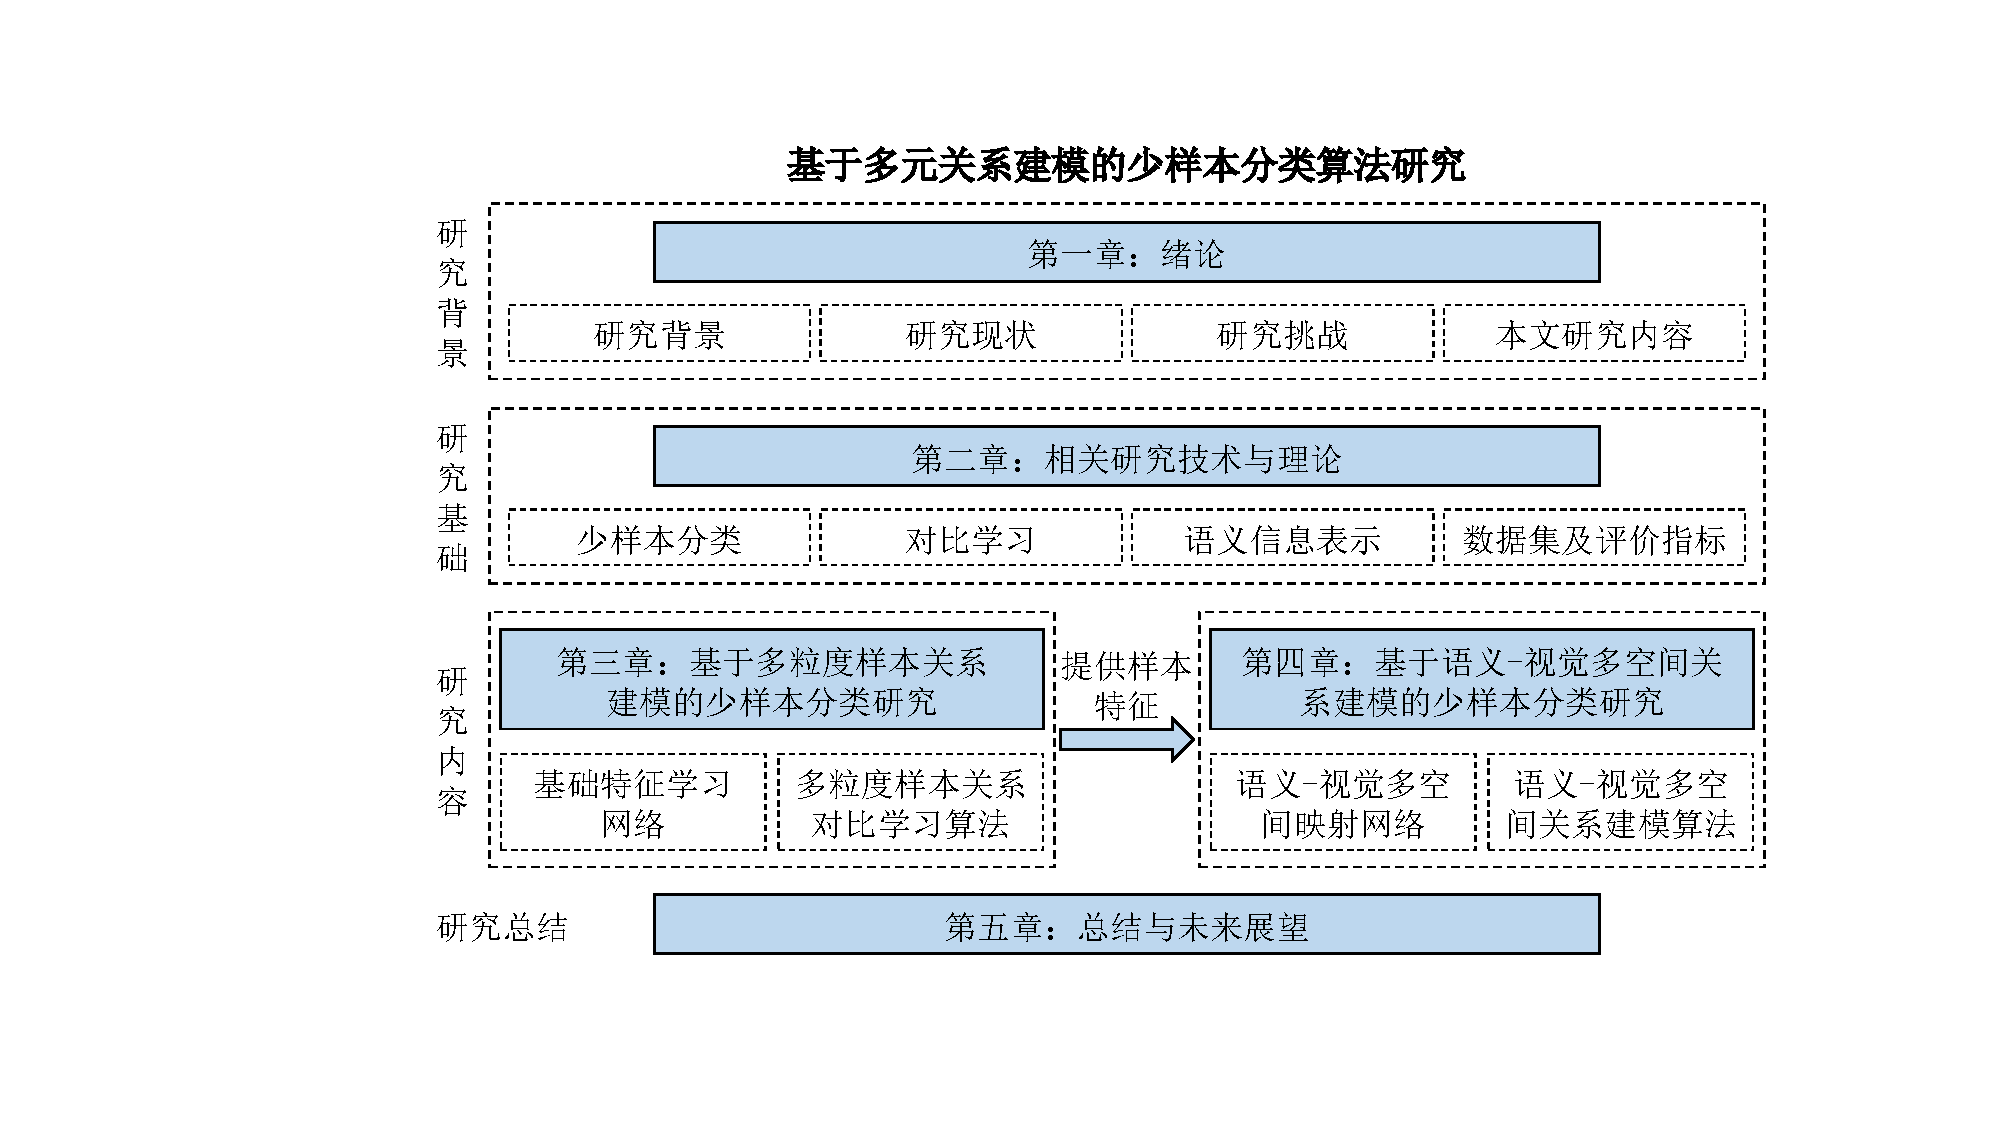
\includegraphics[width=1.0\columnwidth]{figures/组织结构.pdf}
%   \bicaption[本文组织结构图]{本文组织结构图。}[The organizational structure of the paper]{The organizational structure of the paper.}
%   \label{figure1: 组织结构}
% \end{figure}

% \section[\hspace{-2pt}本文组织结构]{{\heiti\zihao{-3} \hspace{-8pt}本文的组织结构}}\label{section1: 本文组织结构}

% 本文的组织结构图如图\ref{figure1: 组织结构}所示,共分为5个章节,各章节的介绍如下:

% 第一章:绪论。介绍少样本分类的研究背景和意义,并分析总结少样本分类算法的国内外研究现状及存在的挑战。最后对本文的研究内容和组织结构进行概述。

% 第二章:相关研究技术与理论。首先对少样本分类进行了进一步详细介绍,然后介绍本文方法中所使用到的对比学习技术以及语义信息表示,最后对本文实验所使用到的数据集及评价指标进行介绍。

% 第三章:基于多粒度样本关系建模的少样本分类研究。首先对部分现有少样本特征学习算法的不足进行分析,提出了基于多粒度样本关系对比学习的少样本特征学习算法(MGSRCL),随后详细介绍了针对不同粒度样本关系的建模方法,最后通过在四个基准数据集的大量实验证明了MGSRCL模型的有效性。

% 第四章:基于语义-视觉多空间关系建模的少样本分类研究。首先对基于语义的少样本分类算法进行分析介绍,提出了基于语义-视觉多空间关系建模的少样本特征适配算法(SVMSMA),然后介绍了SVMSMA模型的模型框架以及提出的跨模态分类和跨模态特征对齐模块,最后对所提方法进行了实验分析。

% 第五章:总结与未来展望。总结并分析了本文提出的基于多元关系建模的少样本分类算法研究的成果及不足,并对未来的研究方向与内容进行了展望。

\chapter[\hspace{0pt}相关研究技术与理论]{{\heiti\zihao{3}\hspace{0pt}相关研究技术与理论}}

\removelofgap
\removelotgap

本章内容共分为五节,\hyperref[section2: 少样本分类]{第一节}详细介绍少样本分类任务;\hyperref[section2: 对比学习]{第二节}介绍与第三章方法相关的对比学习工作;\hyperref[section2: 语义信息表示]{第三节}介绍第四章方法应用到的语义信息表示及一些用来获得语义信息的自然语言处理模型和多模态模型;\hyperref[section2: 数据集及评价指标]{第四节}对本文所使用的数据集和评价指标进行介绍,\hyperref[section2: 本章小结]{第五节}对本章进行小结。

\section[\hspace{-2pt}少样本分类]{{\heiti\zihao{-3} \hspace{-8pt}少样本分类}}\label{section2: 少样本分类}

少样本分类,旨在模拟人类识别新类别的过程,希望模型在拥有大规模标注数据的类别上进行训练之后,能够总结并迁移所学知识到新的类别,以实现在新类别上仅用少量标注数据进行训练便能够达到良好效果的目的。与常规分类任务将数据集划分为训练集与测试集不同,少样本分类数据集被划分为基类数据和新类数据,两者类别互不相交。其中,基类数据与普通分类任务的训练集一致,所有数据均可以被用来训练模型,无论是以元学习还是以普通分类任务的训练方式。而新类数据则是用来测试模型性能,在少样本分类的测试过程中,会在新类数据集上随机采样大量分类任务,每个任务的数据又被划分为支持集与查询集,如图\ref{figure2: 少样本分类测试任务}所示。其中,支持集数据为带有标注的样本,可用来微调整个模型和重新训练分类器,而查询集作用则是类似普通分类任务中的测试集,用来评估模型准确率。根据采样任务中类别数目\emph{N}和样本数目\emph{K}的多少,其又可被称为\emph{N}-way \emph{K}-shot任务,\emph{N}通常取5,\emph{K}通常取1或5。最终,通过对大量采样任务分别进行评估,并计算这些任务的平均准确率作为模型性能的最终评价指标。

\begin{figure}[h!]
\centering
\captionsetup{font={small, stretch=1.312}}
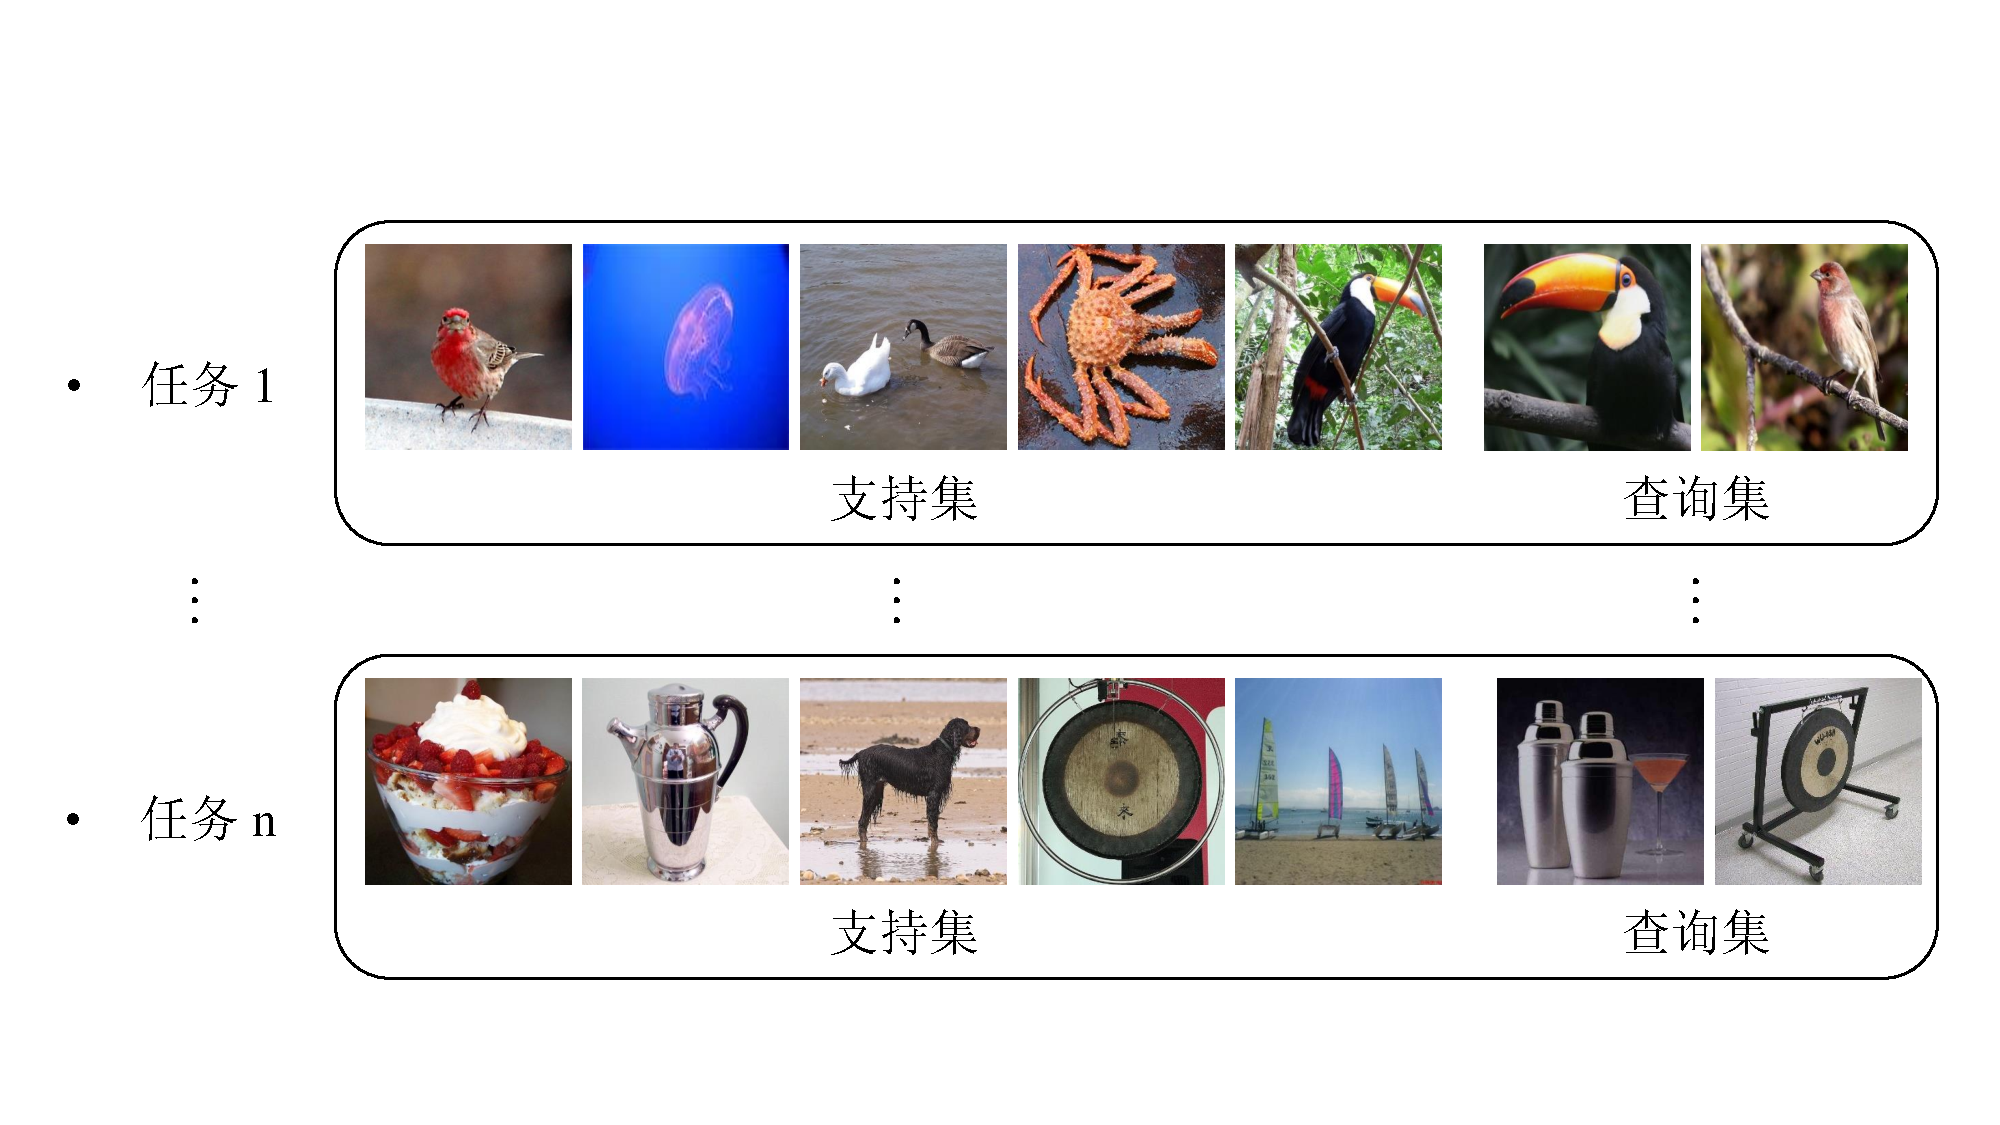
\includegraphics[width=1.0\columnwidth]{figures/RelatedWork/少样本分类测试任务.pdf}
\bicaption[少样本分类测试任务示意图]{少样本分类测试任务示意图。}[Illustration of few-shot classification testing tasks]{Illustration of few-shot classification testing tasks.}
\label{figure2: 少样本分类测试任务}
\end{figure}

\section[\hspace{-2pt}对比学习]{{\heiti\zihao{-3} \hspace{-8pt}对比学习}}\label{section2: 对比学习}

在计算机视觉领域,特征学习的方法越来越多样化。其中,对比学习以其独特的学习机制,即通过比较样本之间的相似性和差异性来提取鲜明且有区分度的特征表征,近年来受到了广泛的关注和研究。在图像处理任务中,对比学习已经证明了其在提高模型泛化能力和识别精度方面的显著效果,并被广泛应用到少样本分类问题中。根据对比学习是否使用数据集标签信息,可以将其分为无监督对比学习和有监督对比学习,以下将分别进行介绍。

\subsection[\hspace{-2pt}无监督对比学习]{{\heiti\zihao{4} \hspace{-8pt}无监督对比学习}}\label{section2: 无监督对比学习}

无监督对比学习不依赖于标注数据,它通常采用正负样本对的形式来构建训练任务。正样本对通常来自于同一实例的不同视角(例如,同一图像的不同数据增强版本),而负样本对则来自于不同实例。模型的目标是使得正样本对在表示空间中彼此接近,而负样本对彼此远离。该过程一般通过最小化InfoNCE损失函数实现,该损失函数如下式所示,
\begin{equation}
\label{equation2: infoNCE}
\mathcal{L} = - \text{log}\frac{\text{exp}(cos(f(x), f(x^+)) / \tau)}{\text{exp}(cos(f(x), f(x^+)) + \sum_{j=1}^{N} \text{exp}(cos(f(x), f(x^-))}.
\end{equation}
其中,图像$x$经由网络$f(\cdot)$后映射到特征空间,$x^+$,$x^-$分别代表$x$的正样本以及负样本,$N$为负样本数量。$cos(\cdot)$是余弦相似度,$\text{exp}(\cdot)$为以e为底的指数函数。

Chen等人\cite{SimCLR}提出了一个简单有效的无监督对比学习框架-SimCLR,旨在通过比较不同视角下图像的特征表示来学习强大的特征提取网络。SimCLR的核心思想是利用数据增强来产生正样本对,即从同一张图像中通过随机的数据增强操作(如裁剪、颜色变换等)生成两个视角,然后使来自同一图像的特征相互靠近,同时使得来自不同图像的特征尽可能地远离。尽管SimCLR在无监督特征学习方面取得了显著的成果,但其有一个明显缺点,即SimCLR的效果很大程度上依赖于对比损失函数中大量不同的负样本对,为了达到最佳性能,需要批次大小很大,这对计算资源的要求较高。He等人\cite{MoCo}提出的MoCo算法通过引入一个动态字典来存储样本特征表示解决了此问题。这个字典是一个队列,新的样本特征进入队列时,旧的样本特征被移除,以保持队列的固定大小。MoCo可通过此字典高效地采样大量负样本,因此不再需要使用很大的批次便可达到最佳效果。这些无监督对比学习方法特别适合于数据量大但未标注的场景,能够有效地利用大量未标注数据来学习有意义的特征表示。

% 通过无监督对比学习,模型能够捕捉到数据的内在结构和丰富的特征信息,这为后续的监督学习任务,如分类、检测等,提供了强大的预训练模型。此外,该方法也在自然语言处理、图数据分析等领域展现出了广泛的应用潜力。

\subsection[\hspace{-2pt}有监督对比学习]{{\heiti\zihao{4} \hspace{-8pt}有监督对比学习}}\label{section2: 有监督对比学习}

虽然无监督对比学习为使用大量无标注数据训练一个好的预训练模型提供了有效途径,但因为其在样本建模过程中将样本$x$与其负样本距离推远,而负样本中可能包含$x$的同类样本,这可能会学习到错误的样本关系。因此,Khosla等人\cite{SupCon}提出了有监督对比学习(Supervised Contrastive Learning,简称SupCon)对这个问题进行解决。SupCon是对比学习的一种变体,它结合了监督信号来进一步提升学习效率和特征表示的质量。与无监督对比学习相比,有监督对比学习在构造正负样本对时利用了标签信息,以确保模型不仅学会区分不同的样本,而且能够区分不同的类别,如图\ref{figure2: 对比学习}所示(此图来源于SupCon\cite{SupCon})。SupCon不仅保留了无监督对比学习中正样本对的概念,更进一步地,将属于同一类别的不同样本也视为正样本对,负样本对则是来自不同类别的样本,以此强化模型对不同类别间差异的识别能力。这种方法有效地缩小了同类样本间的表征距离,同时增强了不同类别间表征的区分度,有助于提升模型在复杂视觉任务中的表现。

\begin{figure}[h!]
\centering
\captionsetup{font={small, stretch=1.312}}
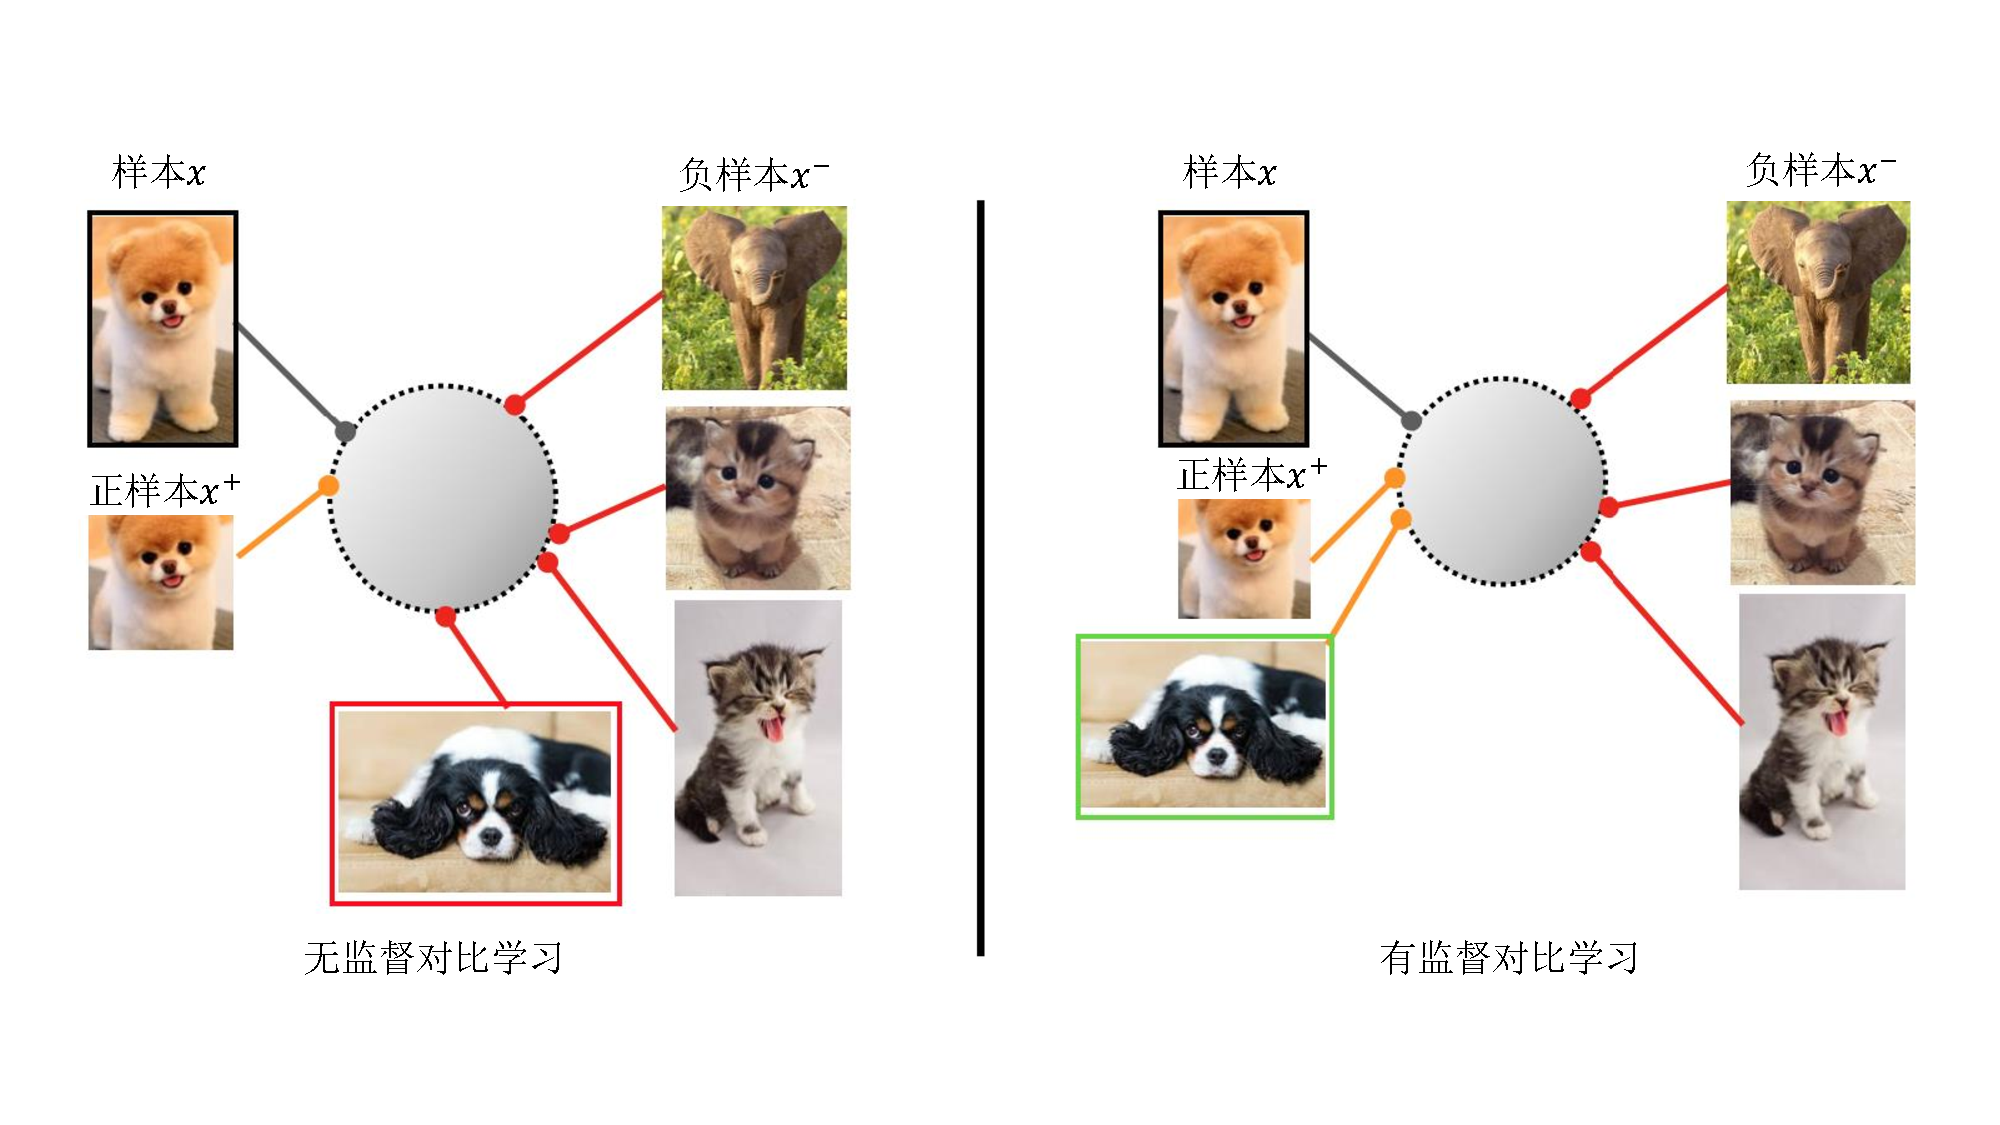
\includegraphics[width=1.0\columnwidth]{figures/RelatedWork/对比学习.pdf}
\bicaption[无监督对比学习与有监督对比学习]{无监督对比学习与有监督对比学习。}[Unsupervised Contrastive Learning VS Supervised Contrastive Learning]{Unsupervised Contrastive Learning VS Supervised Contrastive Learning.}
\label{figure2: 对比学习}
\end{figure}

\section[\hspace{-2pt}语义信息表示]{{\heiti\zihao{-3} \hspace{-8pt}语义信息表示}}\label{section2: 语义信息表示}

目前,在少样本分类问题中,很多工作开始使用语义信息以对视觉信息进行补充,使用的语义信息一般为用自然语言处理(Natural Language Processing,简称NLP)模型或多模态模型的文本编码器提取的语义特征。提取语义特征时,会将类别名称或提示文本与类别名称进行拼接之后的文本输入文本编码器,然后得到编码器输出的语义向量作为语义特征。以下对少样本分类中经常使用的语义特征提取模型进行介绍。

\subsection[\hspace{-2pt}Word2Vec]{{\heiti\zihao{4} \hspace{-8pt}Word2Vec}}\label{section2: Word2Vec}

Mikolov等人\cite{mikolov2013efficient, Word2Vec}提出的Word2Vec是一种广泛使用的自然语言处理技术,它从大量文本语料中以无监督的方式学习语义知识,旨在将词汇映射到稠密向量空间中,其中语义相似的词汇会在向量空间中彼此接近。Word2Vec包含两种训练模型:连续词袋(Continuous Bag-of-Words,简称CBOW)模型和跳跃(Continuous Skip-gram,简称Skip-Gram)模型,如图\ref{figure2: Word2Vec}所示(此图来源于Word2Vec\cite{Word2Vec})。

\textbf{CBOW模型:}CBOW模型通过上下文(周围的词汇)来预测当前词,如图\ref{figure2: Word2Vec}(左)所示。具体来说,它将上下文中的多个词汇作为输入,并尝试预测在这些上下文词汇中间的目标词汇。这个模型特别适合处理较小的数据集。

\textbf{Skip-Gram模型:}与CBOW相反,Skip-Gram模型使用一个词来预测其周围的上下文,如图\ref{figure2: Word2Vec}(右)所示。给定一个特定的词,目标是预测在一个特定范围内的前后词汇。Skip-Gram模型在处理大数据集时表现更好,尤其是对罕见词汇的表示更为有效。

\begin{figure}[h!]
\centering
\captionsetup{font={small, stretch=1.312}}
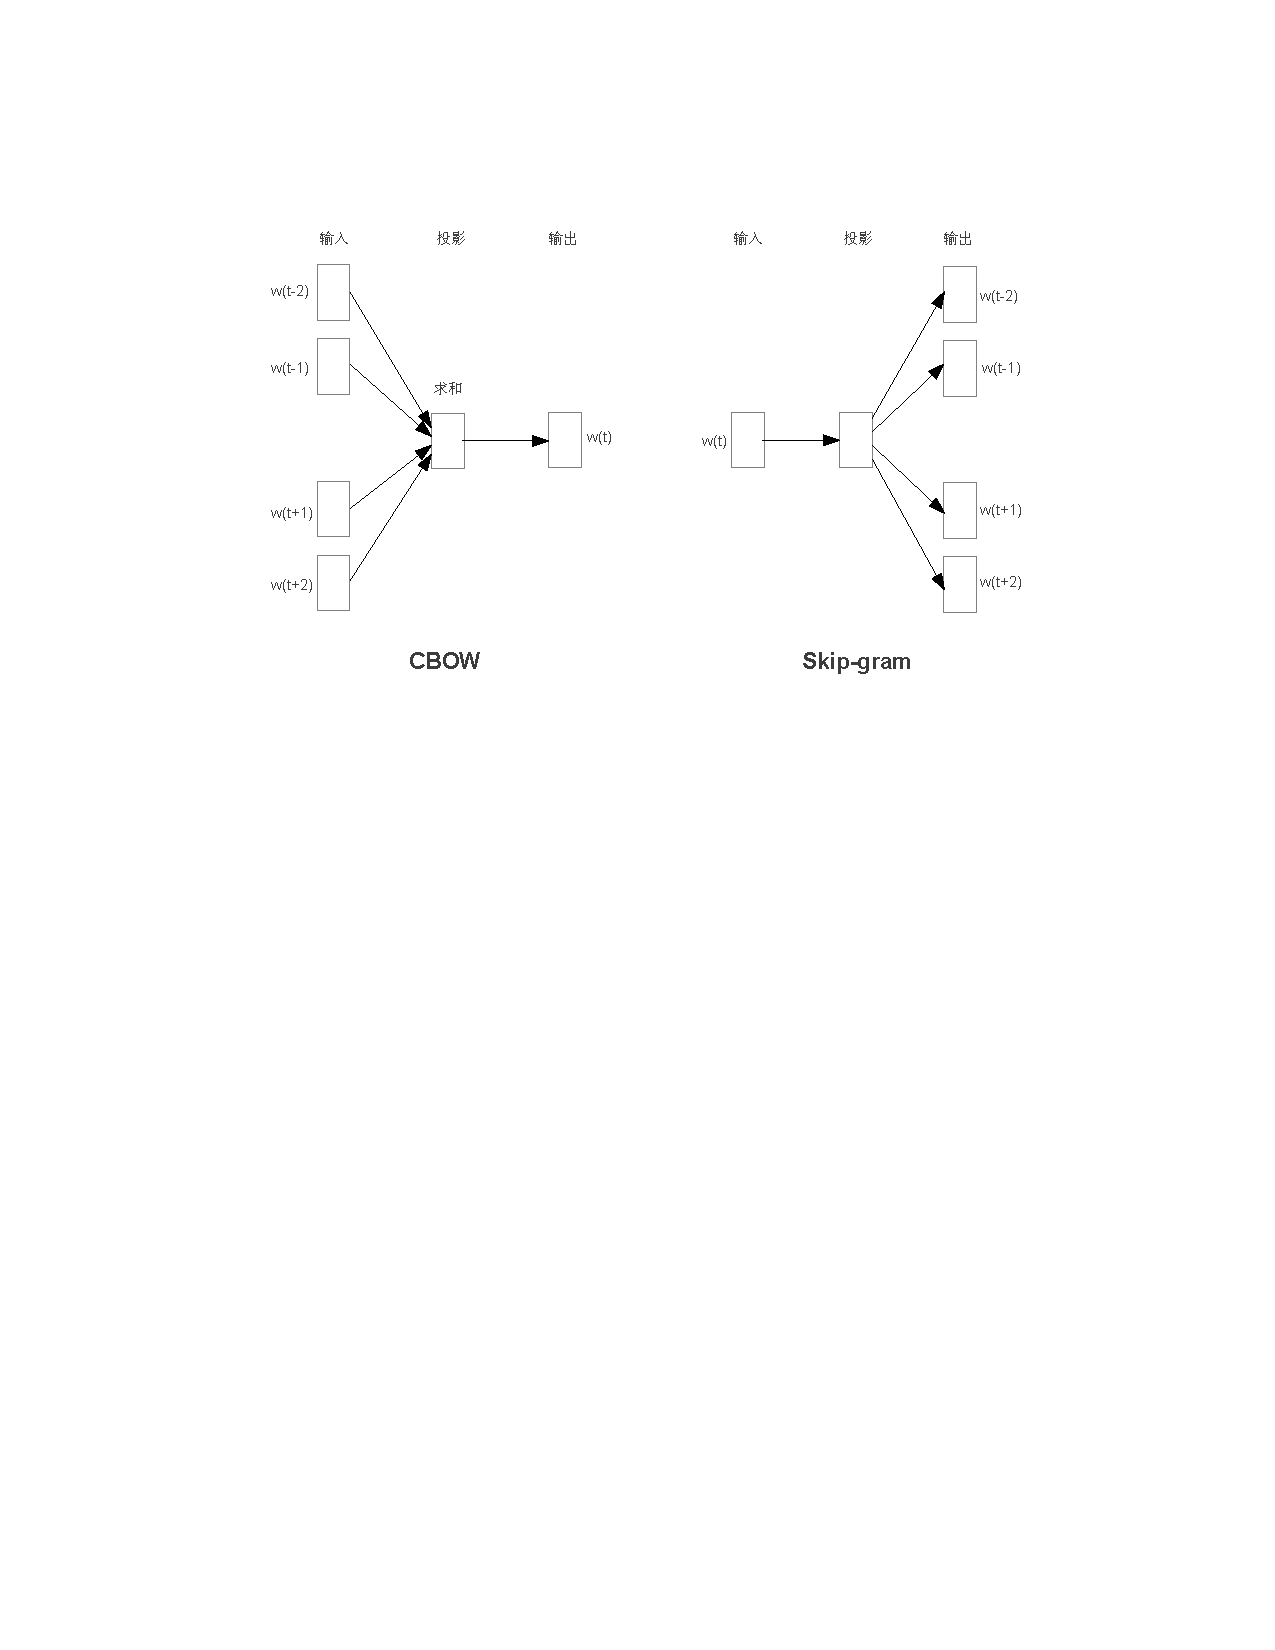
\includegraphics[width=1.0\columnwidth]{figures/RelatedWork/Word2Vec.pdf}
\bicaption[CBOW模型与Skip-Gram模型示意图]{CBOW模型与Skip-Gram模型示意图。}[Illustration of CBOW model and Skip-Gram model]{Illustration of CBOW model and Skip-Gram model.}
\label{figure2: Word2Vec}
\end{figure}

Word2Vec的核心优势在于它能够捕捉到词汇之间的细微语义关系,并通过向量运算来揭示词汇之间的语义相似性。这使得Word2Vec在诸多自然语言处理任务中得到广泛应用,包括文本相似性度量、情感分析、机器翻译以及作为深度学习模型的预训练层等,另外,很多计算机视觉任务也使用Word2Vec来提取语义特征以对视觉特征进行修正或补充。

\subsection[\hspace{-2pt}GloVe]{{\heiti\zihao{4} \hspace{-8pt}GloVe}}\label{section2: GloVe}

Pennington等人\cite{GloVe}提出的GloVe(Global Vectors for Word Representation)也是一种用于词嵌入的无监督学习算法。该模型旨在将单词映射到一个向量空间中,使得这些向量能够捕捉到词与词之间的共现关系,从而反映出词义的复杂模式和结构。GloVe模型的关键创新在于它结合了两种主流的词表示方法的优点:基于全局矩阵分解(Global Matrix Factorization)的方法和基于局部上下文窗口(Local Context Window)的方法。

GloVe的核心思想是首先构建一个全局词共现矩阵,记录整个语料库中各个词之间的共现次数,然后通过优化一个目标函数来学习词向量。这个目标函数旨在让共现次数的对数值与相应词向量的点积尽可能接近,同时引入偏置项来进一步提升模型的灵活性和准确性。具体来说,GloVe构建一个大型的词-词共现矩阵,矩阵中的每个元素代表了两个词在一定窗口大小内共同出现的次数。这一步捕获了全局的共现统计信息。然后其定义了一个特殊的损失函数,该损失函数不仅关注词对之间的共现概率,而且关注共现概率的比例,这有助于捕获词义之间更细微的差别。这个损失函数同时考虑到了共现次数的稀疏性和不均匀性。通过最小化损失函数,模型学习到的词向量能够反映出词与词之间的共现概率,这意味着词向量空间中的距离可以表示词义之间的相似度。这一步既利用了局部信息(通过具体的共现频率),也综合了全局信息(通过整个语料库的统计数据)。

\begin{figure}[h!]
\centering
\captionsetup{font={small, stretch=1.312}}
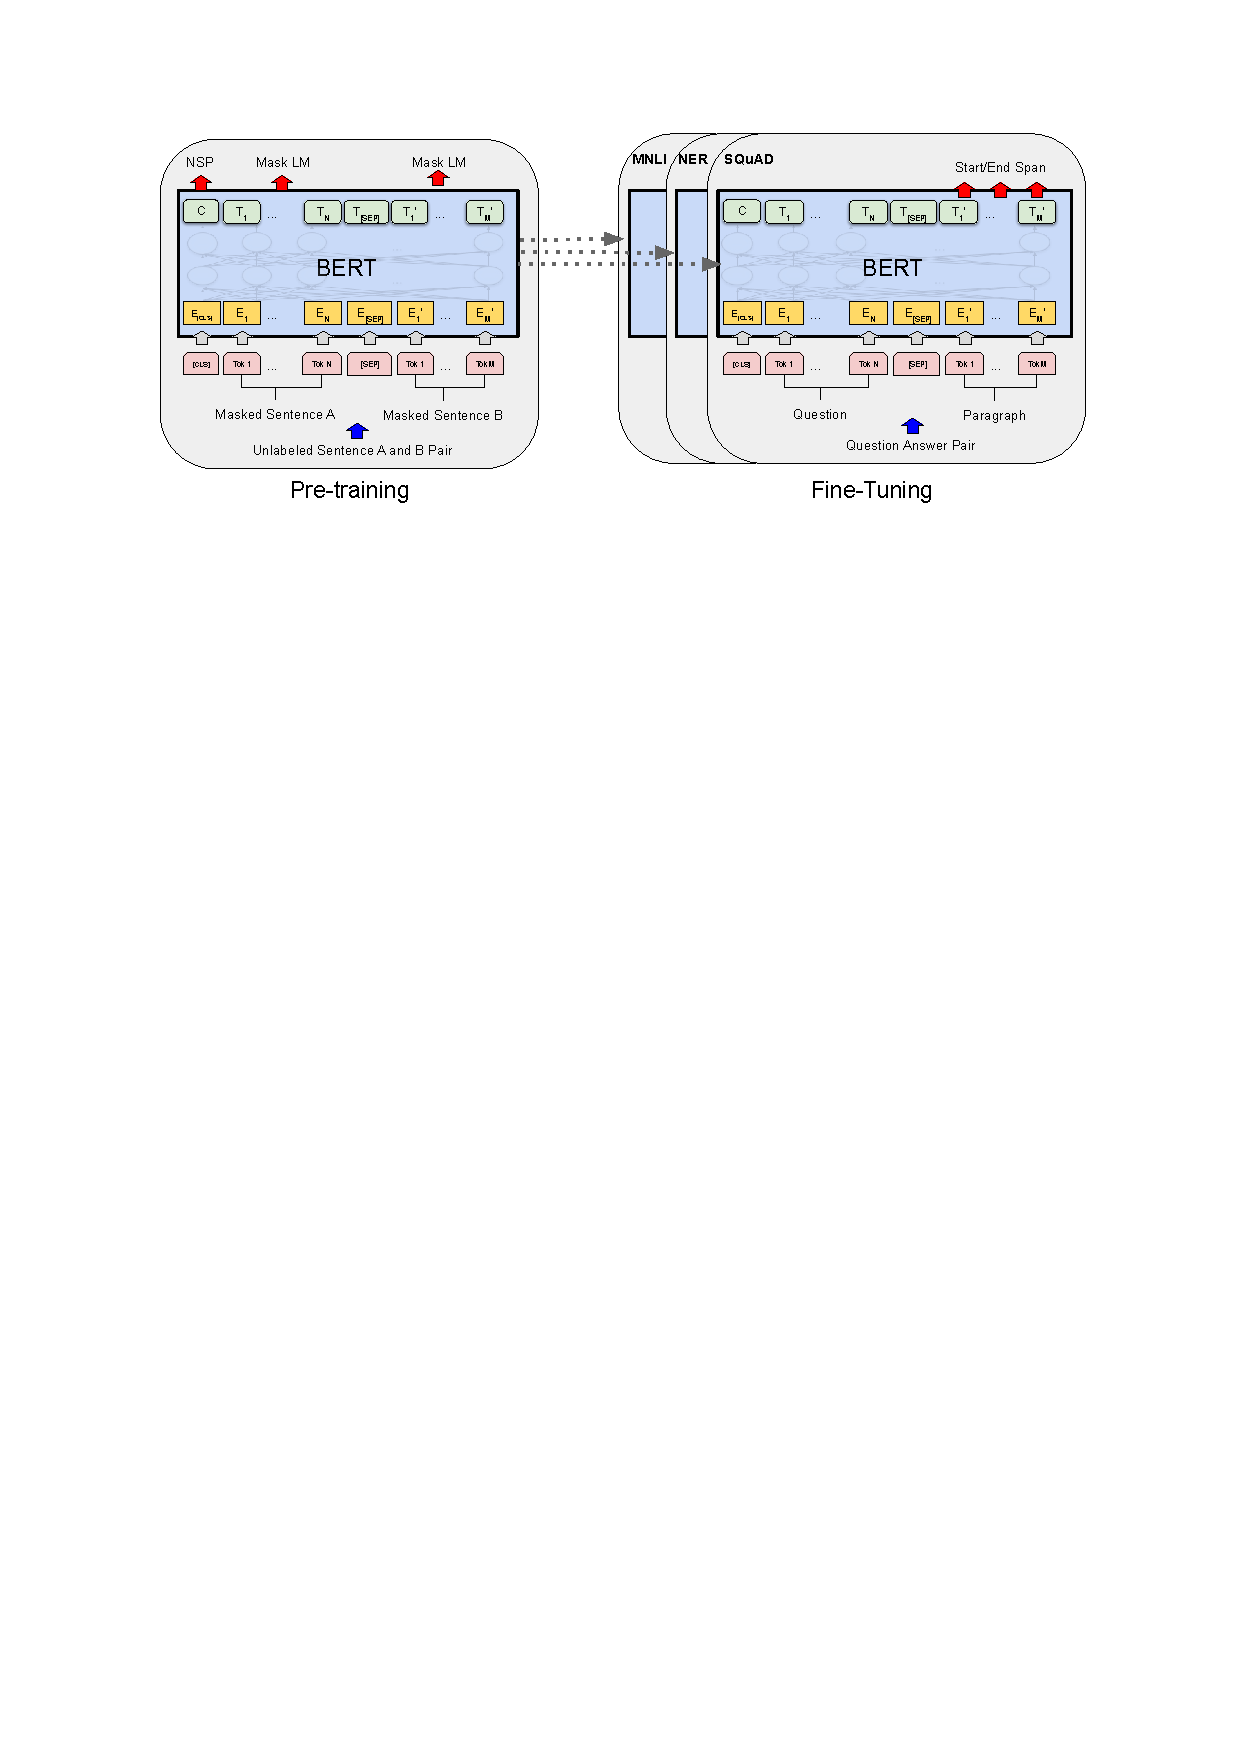
\includegraphics[width=1.0\columnwidth]{figures/RelatedWork/BERT.pdf}
\bicaption[BERT的整体预训练和微调过程]{BERT的整体预训练和微调过程。}[Overall pre-training and fine-tuning procedures for BERT]{Overall pre-training and fine-tuning procedures for BERT.}
\label{figure2: BERT}
\end{figure}

\subsection[\hspace{-2pt}BERT]{{\heiti\zihao{4} \hspace{-8pt}BERT}}\label{section2: BERT}

Devlin等人\cite{Bert}提出的BERT(Bidirectional Encoder Representations from Transformers)模型是一种革命性的自然语言处理模型。该模型利用了Transformer架构的双向编码器,能够理解语言的深层语义和上下文关系。BERT的创新之处在于其基于Transformer模型的编码器,使得它能够同时考虑词语左侧和右侧的上下文信息,这与以往的单向模型或浅层双向模型不同,使其能够更准确地理解词义。如图\ref{figure2: BERT}所示(此图来源于BERT\cite{Bert}),BERT模型首先在大规模的文本语料库上进行预训练,学习通用的语义表示,然后针对具体的NLP任务进行微调,这一过程极大提升了模型在特定任务上的性能。由于其良好的性能与开创性,后续又出现了诸如SBERT\cite{SBERT}、RoBERTa\cite{RoBERTa}、ALBERT\cite{ALBERT}等改进工作。BERT模型通过两种类型的预训练任务学习语义表示:

\noindent \textbf{(1)掩码语言模型(Masked Language Model,简称MLM):}在训练过程中,BERT会随机遮蔽模型输入句子中的一部分词语(使用[MASK] token代替原有输入),然后让模型预测这些遮蔽的词语,这可以迫使模型学习到词语的双向上下文关系。另外,为了解决模型微调期间从未看到[MASK] token的问题,BERT模型不总是直接用[MASK] token代替所选单词,而是将所选单词80\%的概率替换为[MASK] token,10\%的概率用一个随即单词替换所选单词,剩下10\%的概率则是保持其不变。

\noindent \textbf{(2)下一句预测(Next Sentence Prediction,简称NSP):}由于很多NLP下游任务都是基于理解两个句子之间的关系,如问答和自然语言推断,因此BERT设计了一个下一句预测的任务。给定两个句子A和B,模型需要预测B是否是A的下一句,这可以帮助模型理解句子间的关系。

\begin{figure}[h!]
\centering
\captionsetup{font={small, stretch=1.312}}
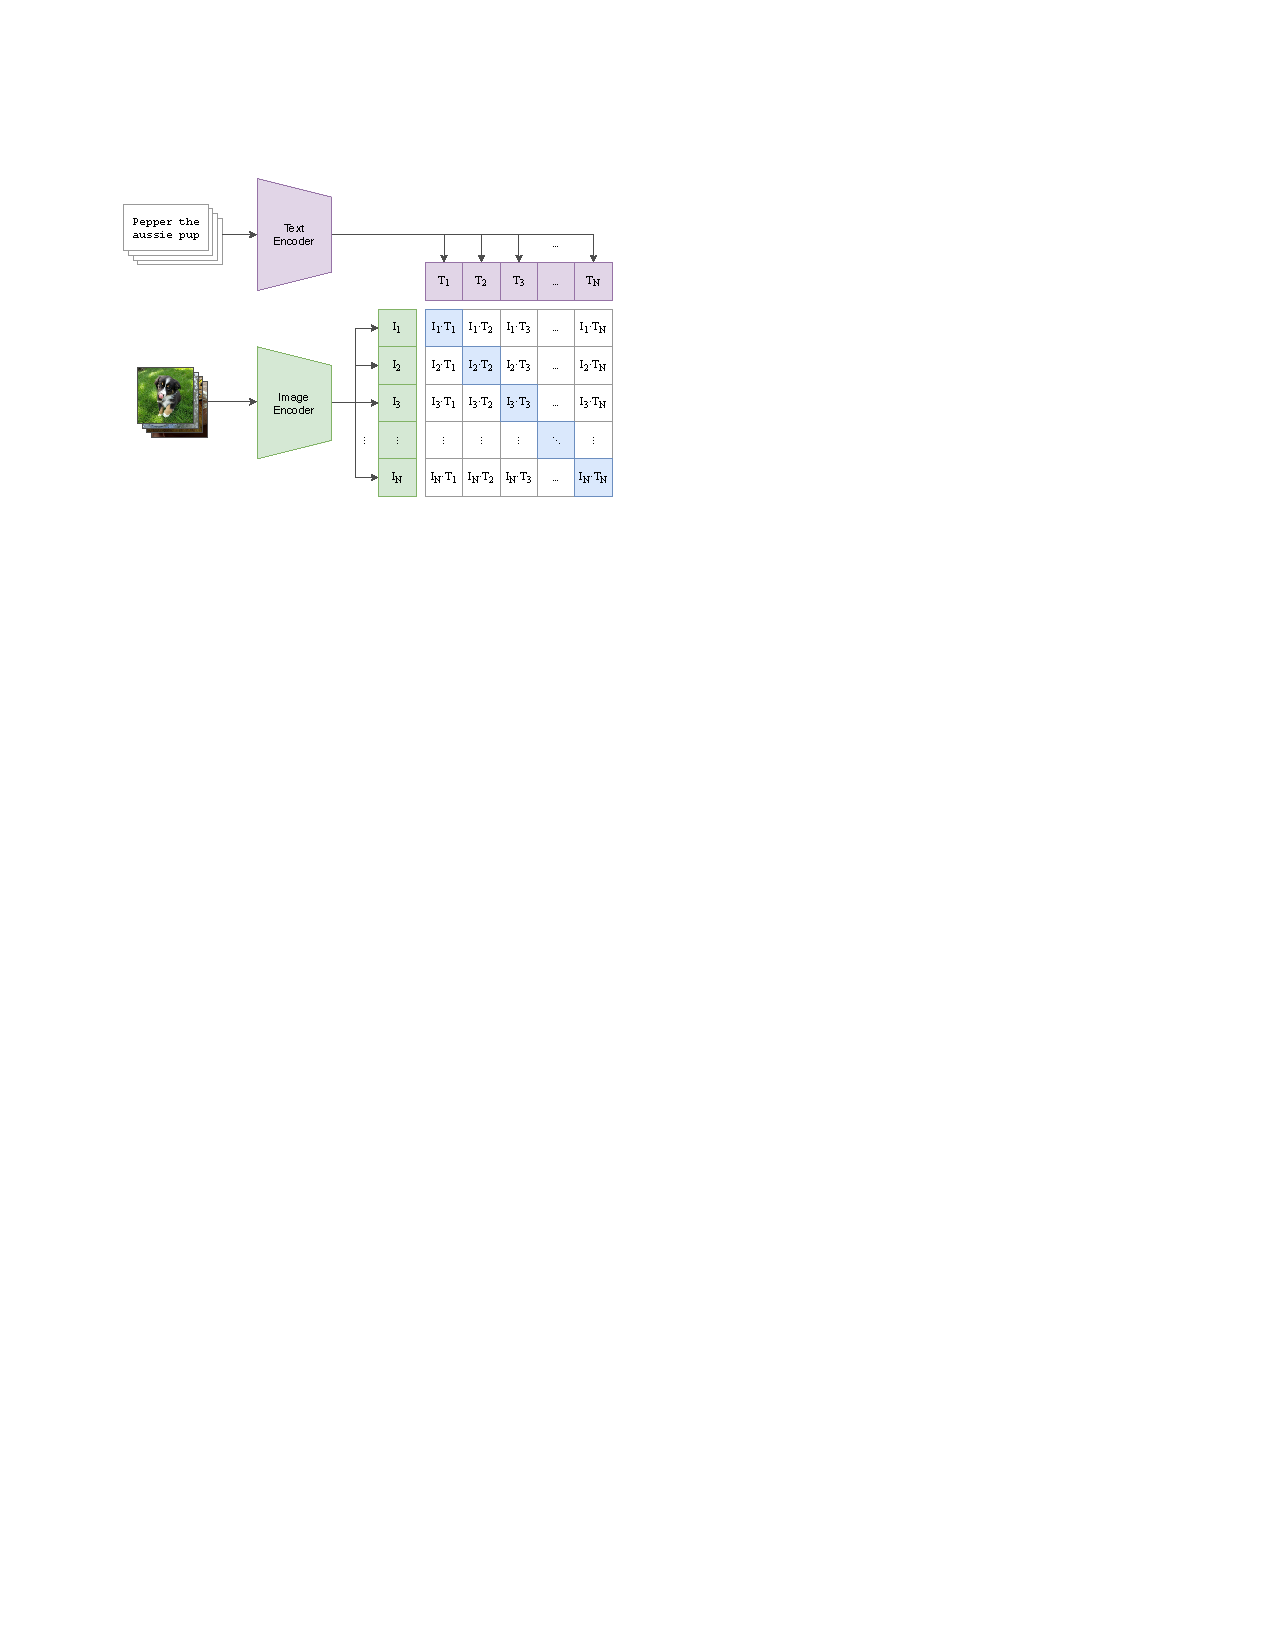
\includegraphics[width=0.8\columnwidth]{figures/RelatedWork/CLIP.pdf}
\bicaption[CLIP模型预训练示意图]{CLIP模型预训练示意图。}[Illustration of pre-training CLIP model]{Illustration of pre-training CLIP model.}
\label{figure2: CLIP}
\end{figure}

\subsection[\hspace{-2pt}CLIP]{{\heiti\zihao{4} \hspace{-8pt}CLIP}}\label{section2: CLIP}

近年来,Radford等人\cite{Clip}提出的CLIP(Contrastive Language–Image Pre-training)模型受到了很多研究者的关注,并促进了多模态大模型和一些其他任务的发展。CLIP旨在通过大规模的图文对比学习来同时理解图像和文本,并建立它们之间的联系。CLIP模型的创新之处在于其跨模态能力,它不仅能理解图片内容,也能理解与图片内容相对应的文本描述,从而在多种视觉任务上展示出了卓越的性能和强大的泛化能力,并提供了一个充分建模文本关系的文本编码器。

如图\ref{figure2: CLIP}所示(此图来源于CLIP\cite{Clip}),CLIP由两部分组成:一个图像编码器和一个文本编码器。图像编码器负责提取图像的视觉特征,而文本编码器则提取文本的语义特征。这两个编码器可以是任何形式的神经网络。在原始CLIP模型中,图像编码器基于Vision Transformer(ViT)或ResNet架构,而文本编码器基于Transformer架构。CLIP的训练过程涉及大量图像和文本对的对比学习。具体来说,模型训练的目标是最大化相匹配的图像和文本对之间的相似度,同时最小化不匹配对的相似度。这种训练方式使得CLIP学习到的特征表示能够跨越视觉和语义的界限,理解两种模态之间的对应关系。

\section[\hspace{-2pt}数据集及评价指标]{{\heiti\zihao{-3} \hspace{-8pt}数据集及评价指标}}\label{section2: 数据集及评价指标}

本文使用四个少样本分类基准数据集对模型性能进行评估,包括三个普通少样本分类数据集:miniImageNet \cite{vinyals2016matching}、tieredImageNet \cite{ren2018meta}、CIFAR-FS \cite{bertinetto2019meta},以及一个细粒度数据集:CUB-200-2011(CUB)\cite{wah2011caltech},以下对其进行分别介绍,并对少样本分类评价指标进行描述。

\begin{table}[h!]
\small    % 设置表格字体为5号
\setstretch{1.245}        % 设置具有指定弹力的橡皮长度(原行宽的1.2倍)
\captionsetup{font={small, stretch=1.512}}
\centering
\bicaption[miniImageNet、CIFAR-FS和CUB的数据集划分]{miniImageNet、CIFAR-FS和CUB的数据集划分。}[Dataset partition of miniImageNet, CIFAR-FS and CUB]{Dataset partition of miniImageNet, CIFAR-FS and CUB.}    % 中英文标题
\begin{tabularx}{\textwidth}{lCCCC}
\toprule
\multirow{2}*{数据集} & \multicolumn{4}{c}{类别数目} \\
\cline{2-5}
& \raisebox{-2pt}{训练集} & \raisebox{-2pt}{验证集} & \raisebox{-2pt}{测试集} & \raisebox{-2pt}{总数} \\
\midrule
miniImageNet & 64 & 16 & 20 & 100 \\
CIFAR-FS & 64 & 16 & 20 & 100 \\
CUB & 100 & 50 & 50 & 200 \\
\bottomrule
\end{tabularx}
\vspace{-20pt}
\label{table2: dataset1}
\end{table}

\begin{table}[h!]
\small    % 设置表格字体为5号
\setstretch{1.245}        % 设置具有指定弹力的橡皮长度(原行宽的1.2倍)
\captionsetup{font={small, stretch=1.512}}
\centering
\bicaption[tieredImageNet的数据集划分]{tieredImageNet的数据集划分。}[Dataset partition of tieredImageNet]{Dataset partition of tieredImageNet.}    % 中英文标题
\begin{tabularx}{\textwidth}{XCCCC}
\toprule
\multirow{2}*{类别层级} & \multicolumn{4}{c}{类别数目} \\
\cline{2-5}
& \raisebox{-2pt}{训练集} & \raisebox{-2pt}{验证集} & \raisebox{-2pt}{测试集} & \raisebox{-2pt}{总数} \\
\midrule
超类 & 20 & 6 & 8 & 34 \\
子类 & 351 & 97 & 160 & 608 \\
\bottomrule
\end{tabularx}
\label{table2: dataset2}
\end{table}

\subsection[\hspace{-2pt}数据集]{{\heiti\zihao{4} \hspace{-8pt}数据集}}\label{section2: 数据集}

miniImageNet数据集\cite{vinyals2016matching}和tieredImageNet数据集\cite{ren2018meta}均为ImageNet\cite{deng2009imagenet}的子集。其中,miniImageNet数据集包含100个类别,每个类别有600张图像。本文遵循Ravi等人\cite{optimization}提出的划分准则,训练集、验证集和测试集分别包含64、16和20个类别。tieredImageNet数据集则包含34个超类(608个子类),分为20个训练类别(351个子类)、6个验证类别(97个子类)和8个测试类别(160个子类)。CIFAR-FS数据集\cite{bertinetto2019meta}源自CIFAR-100数据集,该数据集包含64个训练类别、16个验证类别和20个测试类别,每个类别同样有600张图像。Caltech-UCSD Birds(CUB)-200-2011(简称CUB)数据集\cite{wah2011caltech}则是一个包含不同种类的鸟类细粒度图像数据集,包含11788个图像样本,分为200个类别。根据Triantafillou等人\cite{triantafillou2017few}的划分准则,该数据集包含100个训练类别、50个验证类别和50个测试类别。各数据集划分如表\ref{table2: dataset1}和\ref{table2: dataset2}所示。

\subsection[\hspace{-2pt}评价指标]{{\heiti\zihao{4} \hspace{-8pt}评价指标}}\label{section2: 评价指标}

对于所有数据集,本文评估5-way 1-shot 以及5-way 5-shot少样本分类任务性能。在一次模型评估中,本文方法采样2000个少样本分类任务,并计算了95\%置信区间的平均分类准确率作为模型的评价指标。在一个少样本分类任务中,每个类别的支持集样本数目为1或5(根据任务决定),查询集样本数目为15,与其他方法\cite{RFS, IER}保持一致。

\section[\hspace{-2pt}本章小结]{{\heiti\zihao{-3} \hspace{-8pt}本章小结}}\label{section2: 本章小结}

本章首先详细介绍了少样本分类任务的定义及其训练测试过程。然后对后续研究工作所涉及到的相关技术进行了介绍,其中包括第三章所使用到的对比学习技术,根据是否使用数据集标签信息将其分为无监督对比学习和有监督对比学习进行了详细阐述;以及第四章所使用到的语义信息表示,介绍了如何提取语义信息表示和少样本分类中常用的语义特征提取模型。最后,介绍了本文方法所使用到的少样本分类数据集和评价指标。

\chapter[\hspace{0pt}基于多粒度样本关系建模的少样本分类研究]{{\heiti\zihao{3}\hspace{0pt}基于多粒度样本关系建模的少样本分类研究}}\label{chapter3: 基于多粒度样本关系建模的少样本分类研究}
\removelofgap
\removelotgap
本章研究基于多粒度样本关系建模的少样本特征学习算法,通过挖掘多种粒度的样本关系并对其进行建模从而增强模型的特征提取能力,进而提升少样本分类任务的准确率。本章内容共分为四节,\hyperref[section3: 引言]{第一节}介绍研究动机和方法概述;\hyperref[section3: 基于多粒度样本关系对比学习的少样本特征学习算法]{第二节}介绍本章提出的基于多粒度样本关系对比学习的少样本特征学习算法;\hyperref[section3: 实验设置及结果分析]{第三节}给出实验设置和结果分析;\hyperref[section3: 本章小结]{第四节}对本章进行小结。

\section[\hspace{-2pt}引言]{{\heiti\zihao{-3} \hspace{-8pt}引言}}\label{section3: 引言}

\subsection[\hspace{-2pt}研究动机]{{\heiti\zihao{4} \hspace{-8pt}研究动机}}\label{section3: 研究动机}

少样本分类旨在模拟人类识别物体的过程,这一目标使其受到了广泛关注,并发展出多种方法。其中基于元学习的方法\cite{MAML, optimization, lee2019meta}是主流少样本分类算法之一,这些方法在训练阶段模拟少样本分类任务,并尝试训练一个基础模型,使其能够迅速适应新任务。基于度量的方法\cite{ProtoNet, vinyals2016matching, DeepEMD, zhu2023light}旨在设计度量函数来计算样本之间的距离或相似度,以能够通过比较样本间距离在少量样本情况下也能有效分类。此外,基于增加额外样本以缓解数据匮乏问题的直觉,许多基于数据增强的方法\cite{IDeMe-Net, DualTriNet, AFHN}被提出,通过合成额外样本来增加样本多样性以提高少样本分类性能。然而,这些方法通常涉及复杂的训练阶段,或者在测试阶段需要添加许多额外样本,这带来了较高的计算成本。

近期研究\cite{dhillon2019baseline, chencloser, RFS}显示,在整个基类数据集上对模型使用分类任务进行完全监督形式的预训练,然后在元测试阶段将模型特征提取网络参数冻结并用来提取图像特征,最后使用提取的特征对每个少样本分类任务训练分类器并进行预测,可以实现与上述复杂少样本方法相媲美的性能。这些工作的成功揭示了特征学习在少样本分类中的重要性。为了获得更好的特征提取网络,众多研究者聚焦于少样本分类的特征学习阶段,并提出了一系列令人印象深刻的工作\cite{RFS, IER, PAL, HandCrafted, Spatial, lee2020self, IEPT, ESPT}。
% 其中,一些方法利用自监督任务来提高网络的特征提取能力\cite{lee2020self, IEPT, ESPT}。例如,ESPT\cite{ESPT}通过最大化原始少样本任务与变换后少样本任务之间的局部空间关系一致性来实现。
其中,很多方法采用对比学习作为辅助任务取得了很好的结果\cite{IER, PAL, Spatial},这是因为对比学习可以缓解网络仅通过交叉熵损失学习基类的最具区分性特征,而忽视获取某些次级区分性特征的问题,通过对样本关系建模提高了网络的特征提取能力以及在新类数据集上的泛化性。例如,IER\cite{IER}利用无监督对比损失来约束图像在不同变换下的不变性。PAL\cite{PAL}使用有监督对比学习\cite{SupCon}对教师模型进行初步训练,随后利用教师模型为学生模型提供软标签。

上述采用对比学习作为辅助任务的方法取得了良好的性能,但它们直接使用无监督或有监督对比学习方法来增强网络的特征提取能力,这可能没有充分挖掘利用样本关系的潜力。无监督对比学习\cite{SimCLR, MoCo}将同一样本的不同变换版本(使用不同的数据增强来获得)视为正样本对,将不同样本视为负样本对,不考虑它们的类别标签。尽管这种方法有效地提升了网络对于不同变换不变性的学习能力,并增加了不同类别样本之间的区分度,但它也无意中将属于同一类别的多个样本在特征空间推得更远,这在一定程度上对特征学习是不利的。有监督对比学习\cite{SupCon}通过确保相同类别的样本比不同类别的样本在特征空间具有更紧密的距离来克服上述问题。但在建模样本关系时,它将样本的变换版本和其他同类样本同等对待,这种策略并不合适,因为样本与其变换版本在语义内容上几乎完全一致,而只与其同类样本共享相似的语义内容。换句话说,在学习的特征空间中,样本应与其变换版本比与同类样本更接近。

\begin{figure}[h!]
\centering
\captionsetup{font={small, stretch=1.312}}
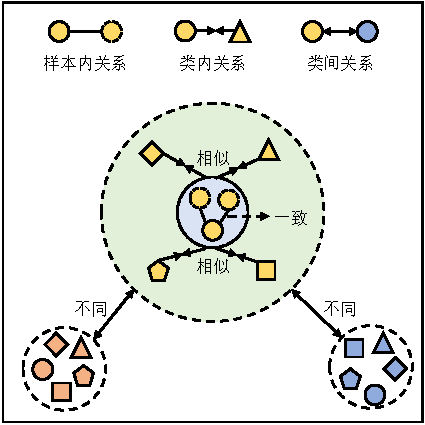
\includegraphics[width=0.6\columnwidth]{figures/MGSRCL/SampleRelation.pdf}
% \captionsetup{justification=justified,singlelinecheck=false}
\bicaption[样本关系示意图]{样本关系示意图。在该图中,不同形状与颜色分别代表不同样本与类别。同一样本的不同变换由相同的颜色和形状表示。样本关系包括三种类型:样本内关系、类内关系和类间关系。本章所提方法约束同一样本不同变换版本在语义内容上保持一致,同类样本保持相似,非同类样本保持不同。}[Illustration of sample relations]{Illustration of sample relations. In this figure, different shapes and different colors represent different samples and different classes, respectively. Different transformations of the same sample are represented by the same color and shape. The sample relations contain three types: intra-sample relation, intra-class relation and inter-class relation. The approach proposed in this chapter enforces different transformations to be consistent in semantic content, homogenous samples to be similar, and inhomogeneous samples to be different.}
\label{figure3: sample relation}
\end{figure}

\subsection[\hspace{-2pt}方法概述]{{\heiti\zihao{4} \hspace{-8pt}方法概述}}\label{section3: 方法概述}

为了解决上述问题,本文重新审视了多种样本关系,并提出了一个针对少样本分类的多粒度样本关系对比学习(Multi-Grained Sample Relation Contrastive Learning, 简称MGSRCL)方法。MGSRCL将样本关系分为三种不同粒度的类型:同一样本不同变换版本的样本内关系(intra-sample relation),同类样本的类内关系(intra-class relation),以及不同类样本的类间关系(inter-class relation),这三种样本关系揭示了数据在不同层次的内在结构和差异,如图\ref{figure3: sample relation}所示。

针对这三种不同粒度的样本关系,MGSRCL提出了两个模块对其进行约束。首先对于同一样本不同变换间的样本内关系,本文通过变换一致性学习(Transformation Consistency Learning,简称TCL)策略进行约束。这一策略的灵感来源于这样一个认识:同一样本在不同但轻微的变换下应保持其本质的语义不变性。TCL通过对齐样本及其变换版本的预测标签分布来确保其在标签输出上的一致性,从而保证样本和其不同变换版本在特征空间保持高度的语义一致性。第二种样本关系是同类样本的类内关系,由于同类样本的语义内容不像同一样本不同变换那样高度一致,忽视同类样本之间的语义差异并将它们映射到特征空间中的同一位置会因为简化了模型的学习过程而导致模型崩塌。因此,本文采用类对比学习(Class Contrastive Learning,简称CCL)来以一种相对的形式约束这种样本关系以及第三种样本关系,即不同类样本的类间关系。CCL不追求同类样本在特征空间中的绝对一致性,而着重于以一种相对距离的方式在特征空间中增强同类样本间的内聚程度,同时增大不同类别间的分离程度,从而提高了模型对不同类别样本的区分能力。

以验证本章方法的有效性,本章在四个基准数据集上进行了广泛的实验,包括三个普通少样本分类数据集:miniImageNet\cite{vinyals2016matching}、tieredImageNet\cite{ren2018meta}、CIFAR-FS\cite{bertinetto2018meta},以及一个细粒度少样本分类数据集:CUB-200-2011\cite{wah2011caltech}。实验结果表明,本章方法取得了优异的结果,并且可以作为预训练模型提升其他两阶段少样本分类方法的性能。


\section[\hspace{-2pt}基于多粒度样本关系对比学习的少样本特征学习算法]{{\heiti\zihao{-3} \hspace{-8pt}基于多粒度样本关系对比学习的少样本特征学习算法}}\label{section3: 基于多粒度样本关系对比学习的少样本特征学习算法}

在本节中,首先对少样本分类任务及其符号定义进行介绍;然后对所提出的基于多粒度样本关系对比学习的少样本特征学习模型进行简要介绍;接下来详细介绍了所提模型的各个模块及其损失优化;最后介绍了模型总体优化目标以及模型推理过程。

\subsection[\hspace{-2pt}符号定义]{{\heiti\zihao{4} \hspace{-8pt}符号定义}}\label{section3: 符号定义}

在本章中,少样本分类任务的基类数据集和新类数据集分别表示为:
\begin{equation}
\begin{aligned}
  &\mathcal{D}_{base} = \{(x, y)|x \in X^{base}, y \in Y^{base}\}, \\
  &\mathcal{D}_{novel} = \{(x, y)|x \in X^{novel}, y \in Y^{novel}\}.
\end{aligned}
\end{equation}
其中,$\mathcal{D}_{base}$所包含的类别$\mathcal{C}_{base}$和$\mathcal{D}_{novel}$所包含的类别$\mathcal{C}_{novel}$不相交。另外,$x$、$y$分别表示样本图像和样本标签;$X^{base}$、$Y^{base}$和$X^{novel}$、$Y^{novel}$分别表示基类数据和新类数据的样本图像集合和标签集合。

$\mathcal{D}_{base}$用于在预训练阶段训练一个具有良好泛化性能的模型,$\mathcal{D}_{novel}$用于测试过程采样大量\emph{N}-way \emph{K}-shot少样本分类任务并计算平均准确率来评估模型性能。每个少样本分类任务$\mathcal{T}$包括一个支持集$\mathcal{S}_\mathcal{T}$和一个查询集$\mathcal{Q}_\mathcal{T}$,
\begin{equation}
  \mathcal{T} = \{\mathcal{S}_\mathcal{T}, \mathcal{Q}_\mathcal{T}\}.
\end{equation}
其中,$\mathcal{S}_\mathcal{T}$包含来自\emph{N}个类别的\emph{N} $\times$ \emph{K}个标注样本,而$\mathcal{Q}_\mathcal{T}$包含来自相同\emph{N}个类别的\emph{N} $\times$ \emph{Q}个样本,并且$\mathcal{S}_\mathcal{T}$和$\mathcal{Q}_\mathcal{T}$中的样本是没有交集的。在测试阶段,针对每个采样的少样本分类任务使用$\mathcal{S}_\mathcal{T}$重新训练一个分类器,使用$\mathcal{Q}_\mathcal{T}$来评估分类器性能。

\begin{figure}[h!]
\centering
\captionsetup{font={small, stretch=1.312}}
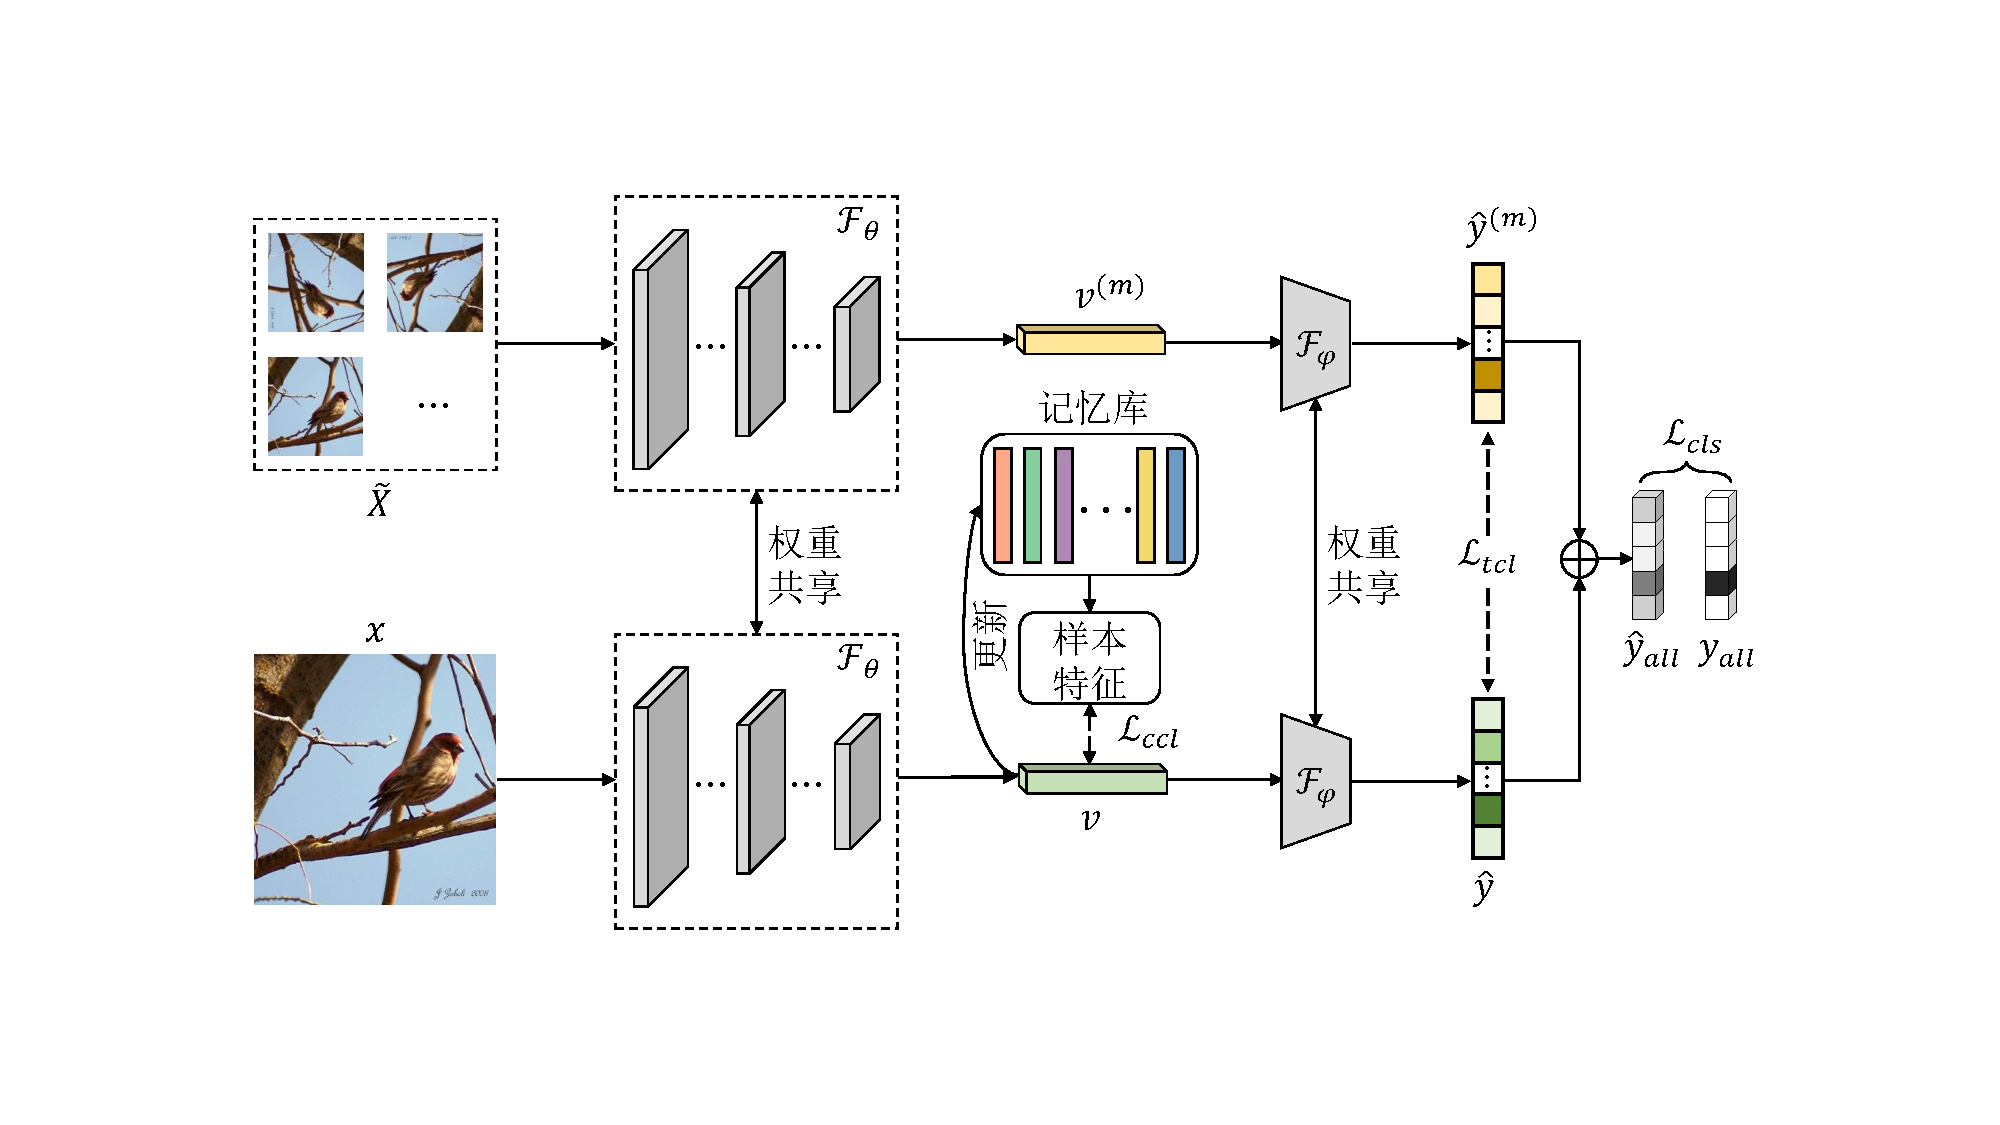
\includegraphics[width=1.0\columnwidth]{figures/MGSRCL/model.pdf}
% \captionsetup{justification=justified,singlelinecheck=false}
\bicaption[多粒度样本关系对比学习模型示意图]{多粒度样本关系对比学习模型(MGSRCL)示意图。它包含一个特征提取网络$\mathcal{F}_{\theta}$和一个分类器$\mathcal{F}_{\varphi}$。在此图中,$v$和$v^{(m)}$代表原始图像$x$及其第$m$个变换版本$x^{(m)}$的特征,其中$x^{(m)} \in \widehat{X}$。$\bigoplus$是一个连接操作,用于对原始图像的预测输出$\widehat{y}$与$M$个变换的预测输出${\widehat{y}^{(1)}, ..., \widehat{y}^{(m)}, ..., \widehat{y}^{(M)}}$进行连接。记忆库(Memory Bank)用于存储特征。$\mathcal{L}_{cls}$,$\mathcal{L}_{tcl}$和$\mathcal{L}_{ccl}$分别是分类损失、变换一致性学习(TCL)损失和类对比学习(CCL)损失。为了便于阅读,此图中没有展示自监督模块。}[Illustration of Multi-Grained Sample Relation Contrastive Learning (MGSRCL) model]{Illustration of Multi-Grained Sample Relation Contrastive Learning (MGSRCL) model. It contains a feature extraction network $\mathcal{F}_{\theta}$ and a classifier $\mathcal{F}_{\varphi}$. In this figure, $v$ and $v^{(m)}$ represent the features of the original image $x$ and its $m$-th transformed version $x^{(m)}$,where $x^{(m)} \in \widehat{X}$. $\bigoplus$ is a concatenation operator for the predicted output $\widehat{y}$ of the original image and the predicted outputs $\{\widehat{y}^{(1)}, ..., \widehat{y}^{(m)}, ..., \widehat{y}^{(M)}$\} of $M$ transformations. Memory bank is used to store the features. $\mathcal{L}_{cls}$, $\mathcal{L}_{tcl}$, and $\mathcal{L}_{ccl}$ are the classification loss, transformation consistency learning (TCL) loss, and class contrastive learning (CCL) loss, respectively. For the sake of legibility, the self-supervised module is not shown in this image.}
\label{figure3: model}
\end{figure}

\subsection[\hspace{-2pt}整体框架]{{\heiti\zihao{4} \hspace{-8pt}整体框架}}\label{section3: 整体框架}

本章重新审视了对比学习中的样本关系,并根据样本关系粒度的不同将其划分为三种类型:同一样本在不同变换下的样本内关系(intra-sample relation)、同类样本的类内关系(intra-class relation),以及不同类样本的类间关系(inter-class relation)。基于此,本章提出了一种新颖的多粒度样本关系对比学习方法(Multi-Grained Sample Relation Contrastive Learning,简称MGSRCL),通过对少样本分类中不同粒度的样本关系进行建模从而获得了一个强大的特征提取网络。如图\ref{figure3: model}所示,MGSRCL模型包含三个主要部分:基础特征学习网络(Base Feature Learning Network,简称Base)、变换一致性学习(Transformation Consistency Learning,简称TCL)模块和类对比学习(Class Contrastive Learning,简称CCL)模块。具体而言,基础特征学习网络是通过一般图像分类任务训练的神经网络。TCL模块旨在确保同一样本的不同变换版本具有一致的语义内容。而CCL则用于确保同类样本具有相似的语义内容,以及非同类样本具有不同的语义内容。接下来,本节将对MGSRCL方法的每个部分进行更为详细的阐述。

\subsection[\hspace{-2pt}基础特征学习网络]{{\heiti\zihao{4} \hspace{-8pt}基础特征学习网络}}\label{section3: 基础特征学习网络}

如图\ref{figure3: model}所示,特征提取网络,表示为带有参数$\theta$的$\mathcal{F}_{\theta}$,被用于提取图像特征。设$(x, y)\in \mathcal{D}_{base}$表示从$\mathcal{D}_{base}$中采样的图像及其对应的标签。图像$x$的特征向量$v$可以通过$\mathcal{F}_{\theta}$获得:$v=\mathcal{F}_{\theta}(x)$。然后,使用参数为$\varphi$的分类器$\mathcal{F}_{\varphi}$,将特征向量$v$投影到标签空间,以获得预测的置信度分数$p$:$p=\mathcal{F}_{\varphi}(v)$。最后,通过在$p$上应用Softmax函数,可以得到预测概率输出$\widehat{y}$:$\widehat{y}=\text{Softmax}(p)$。基础特征学习网络的参数$\theta$和$\varphi$通过最小化整个基类数据集$\mathcal{D}_{base}$上的分类损失$\mathcal{L}_{cls}$来进行优化,其可以表示为以下公式,
\begin{equation}
\label{equation3:3.2}
  \mathcal{L}_{cls} = - \frac{1}{|\mathcal{D}_{base}|}\sum_{\{x,y\}\in \mathcal{D}_{base}}y\log\widehat{y}.
\end{equation}

为了防止在训练集上过拟合,许多方法\cite{IER, PAL, SSLforFSL}引入了变换样本参与训练,并使用自监督学习技术预测在训练过程中对图像执行了哪种变换以增强网络的特征提取能力。遵循这些方法,本文也添加了一个由多层感知机(Multilayer Perceptron,简称MLP)构成的自监督(Self-Supervised,简称SS)模块。设$\widetilde{X}=\{\widetilde{x}^{(1)}, ..., \widetilde{x}^{(M)}\}$为一张图像的变换版本集合,其中$M$表示变换样本的总数,$\widetilde{x}^{(m)}$表示图像的第$m$个变换版本。$\widetilde{X}$可以通过在图像上应用一系列变换(如裁剪、调整大小、旋转等数据增强操作)获得。变换后的图像$\widetilde{X}$和原始图像$x$同时输入模型,用于分类和自监督任务。自监督任务的目标是识别图像进行了哪种变换,其损失$\mathcal{L}_{ss}$表示为以下公式,
\begin{equation}
\label{equation3:3.3}
  \mathcal{L}_{ss} = - \frac{1}{|\mathcal{D}_{base}|}\frac{1}{M+1}\sum_{x \in \mathcal{D}_{base}}\sum_{m=0}^{M}s^{(m)}\log\widehat{s}^{(m)},
\end{equation}
其中$\widehat{s}^{(m)}$和$s^{(m)}$分别表示自监督任务中第$m$个变换版本的预测概率输出和真实标签。$s^{(0)}$是原始图像$x$的自监督标签。此外,增加了变换样本之后的分类损失可以重新定义为以下公式,
\begin{equation}
\label{equation3:3.4}
  \mathcal{L}_{cls} = - \frac{1}{|\mathcal{D}_{base}|}\frac{1}{M+1}\sum_{x \in \mathcal{D}_{base}}\sum_{m=0}^{M}y^{(m)}\log\widehat{y}^{(m)},
\end{equation}
$\widehat{y}^{(m)}$表示分类任务中的预测概率输出,$y^{(m)}$表示分类任务的真实标签。

最后,基础特征学习网络的损失$\mathcal{L}_{base}$可以写为分类损失$\mathcal{L}_{cls}$和自监督损失$\mathcal{L}_{ss}$之和,
\begin{equation}
\label{equation3:3.5}
  \mathcal{L}_{base} = \mathcal{L}_{cls} + \mathcal{L}_{ss}.
\end{equation}

\subsection[\hspace{-2pt}多粒度样本关系对比学习算法]{{\heiti\zihao{4} \hspace{-8pt}多粒度样本关系对比学习算法}}\label{section3: 多粒度样本关系对比学习算法}

\textbf{(1)变换一致性学习}

一个样本图像与其变换版本包含完全相同的对象和背景,仅因为进行了数据增强而使得图像在旋转角度、明暗、颜色等方面发生变化,但其内在的类别属性和语义内容应保持不变。为了实现这一目标,本文设计了一个变换一致性学习(Transformation Consistency Learning,简称TCL)模块,以约束同一样本不同变换版本的样本内关系。TCL模块通过约束一个样本和其变换版本的预测输出相同来确保它们具有一致的语义内容。这是因为预测输出反映了样本在每个类别中的预测概率,这些概率不仅表示了模型对于样本属于各个类别的置信度,而且深入地揭示了样本的本质属性——亦即其语义内容。

本章方法将一个样本与其变换版本同时输入网络,并在预测标签输出层面计算它们的TCL损失。这里,本文使用Jensen-Shannon散度\cite{JS1, JS2}作为TCL损失,它能够衡量两个概率分布的差异,通过最小化两个预测标签的输出,可以使其概率分布一致,从而达到使样本和其变换版本具有一致语义内容的目的。TCL损失可以写为以下公式,
\begin{equation}
\label{equation3:3.6}
  \mathcal{L}_{tcl} = \frac{1}{|\mathcal{D}_{base}|}\sum_{x \in \mathcal{D}_{base}}\frac{1}{M}\sum_{m=1}^{M}JS(\widehat{y}_{\tau_1}, \widehat{y}_{\tau_1}^{(m)}),
\end{equation}
其中$\widehat{y}_{\tau_1}$和$\widehat{y}_{\tau_1}^{(m)}$分别是原始图像和第$m$个变换图像的平滑标签输出。它们通过以下公式获得,
\begin{equation}
\label{equation3:3.7}
  \widehat{y}_{\tau_1} = \text{Softmax}(p/\tau_1),
\end{equation}
此公式中$p = \mathcal{F}_{\varphi}(\mathcal{F}_{\theta}(x))$,$\tau_1$是一个温度参数,本文在实验中将其设置为$4.0$。使用平滑标签输出的原因在于不同变换的输出不仅需要在最大预测概率的类别上保持一致,而且需要在所有其他类别上也保持一致,以确保它们具有完全相同的语义内容,而平滑标签输出可以提供更多关于概率分布差异的信息。

\textbf{(2)类对比学习}

同类样本虽然图像内包含了同一个类别的物体,但物体及其背景与同一图像不同变换版本相比差异性较大,因此其预测概率输出之间差异也会较大。如果强行将其预测输出进行对齐,可能会使得网络为了学习此种强关系而导致模型崩塌。但在另一方面,同类样本间距离比不同类样本间距离更近是毋庸置疑的。因此,本文采用类对比学习(Class Contrastive Learning,简称CCL)以一种相对距离的形式约束同类样本的类内关系和不同类样本的类间关系。CCL模块通过最大化同类样本特征的相似性,同时最小化不同类样本特征的相似性来在特征空间拉近同类样本,推远不同类样本。

与之前对比学习不同,CCL模块为了将样本和其他每个不同类间的距离推远,对于每张图像都需要该图像的一个同类样本以及其他每个类别的不同类样本(之前对比学习通常随机采样,这使得每个批次计算损失时不同类样本可能仅来自部分不同类别)。为了实现这一目标并加快训练速度,本文使用了一个记忆库(Memory Bank)来存储和从中采样图像特征,记忆库存储了所有图像的特征。在一个批次中,CCL模块从记忆库中为每类图像随机采样一个样本的特征。CCL损失可以定义为,
\begin{equation}
\label{equation3:3.8}
  \mathcal{L}_{ccl} = \frac{1}{|\mathcal{D}_{base}|}\sum_{x \in \mathcal{D}_{base}}-\log \frac{\text{exp}(\frac{cos(v, v^\prime)}{\tau_2})}{\sum_{i=1}^{|\mathcal{C}_{base}|}{\text{exp}(\frac{cos(v, v_i)}{\tau_2})}},
\end{equation}
其中$|\mathcal{C}_{base}|$和$|\mathcal{D}_{base}|$表示基类的类别数量和样本数量,$v$和$v^\prime$分别是某个样本及其同类样本的特征,$v_i$代表来自第$i$类的样本的特征。这里$v^\prime$和$v_i$是从记忆库中采样的。$cos(\cdot)$是余弦相似度,$\text{exp}(\cdot)$为以e为底的指数函数。而$\tau_2$是一个温度参数,本文按照\cite{SimCLR, SupCon}的实验设置将其设为$0.1$。此外,记忆库的更新方式为,
\begin{equation}
\label{equation3:3.9}
  v_{k} = r\times v_k + (1 - r)\times v_q,
\end{equation}
$v_q$和$v_k$分别代表在当前小批次中获得的图像特征以及在记忆库中存储的相同图像的特征,$r$用于调整记忆库的更新速度,按照IER方法\cite{IER}的实验,本文将其设置为$0.99$。在训练阶段,记忆库每一轮训练过程都会完全更新一遍。

\subsection[\hspace{-2pt}模型优化]{{\heiti\zihao{4} \hspace{-8pt}模型优化}}\label{section3: 模型优化}
结合公式\ref{equation3:3.5}、\ref{equation3:3.6}和\ref{equation3:3.8},本章提出的MGSRCL模型总体损失函数可以表示为以下公式,
\begin{equation}
\label{equation3:3.10}
  \mathcal{L}_{total} = \mathcal{L}_{base} + \alpha \cdot \mathcal{L}_{tcl} + \beta \cdot \mathcal{L}_{ccl},
\end{equation}
其中$\alpha$和$\beta$是用于平衡不同损失的超参数,分别表示TCL模块和CCL模块的损失权重。

MGSRCL模型通过在整个基类数据集上最小化上述损失函数对模型参数进行联合优化。通过建模多个粒度的样本关系,可以有效地增强模型的特征提取能力和泛化能力,帮助模型捕获更具判别性的特征,从而提高模型在新类$\mathcal{D}_{novel}$上的分类性能。

\subsection[\hspace{-2pt}模型推理]{{\heiti\zihao{4} \hspace{-8pt}模型推理}}\label{section3: 模型推理}
模型在基类数据集$\mathcal{D}_{base}$训练完成之后,在测试阶段,将会冻结MGSRCL模型特征提取网络的所有参数,并通过解决来自新类$\mathcal{D}_{novel}$的大量少样本分类任务来评估模型性能。在每个任务$\mathcal{T}$的推理过程中,本文使用特征提取网络$\mathcal{F}_{\theta}$来获得支持集$\mathcal{S}_\mathcal{T}$和查询集$\mathcal{Q}_\mathcal{T}$的图像特征。然后,本文使用$\mathcal{S}_\mathcal{T}$的样本特征训练一个逻辑回归分类器$LC$,并对$\mathcal{Q}_\mathcal{T}$中的样本进行分类,最后将在多个少样本分类任务上的准确率平均值作为模型的评价指标。MGSRCL模型的推理过程如图\ref{figure3: 推理过程}所示。

\begin{figure}[h]
\centering
\captionsetup{font={small, stretch=1.312}}
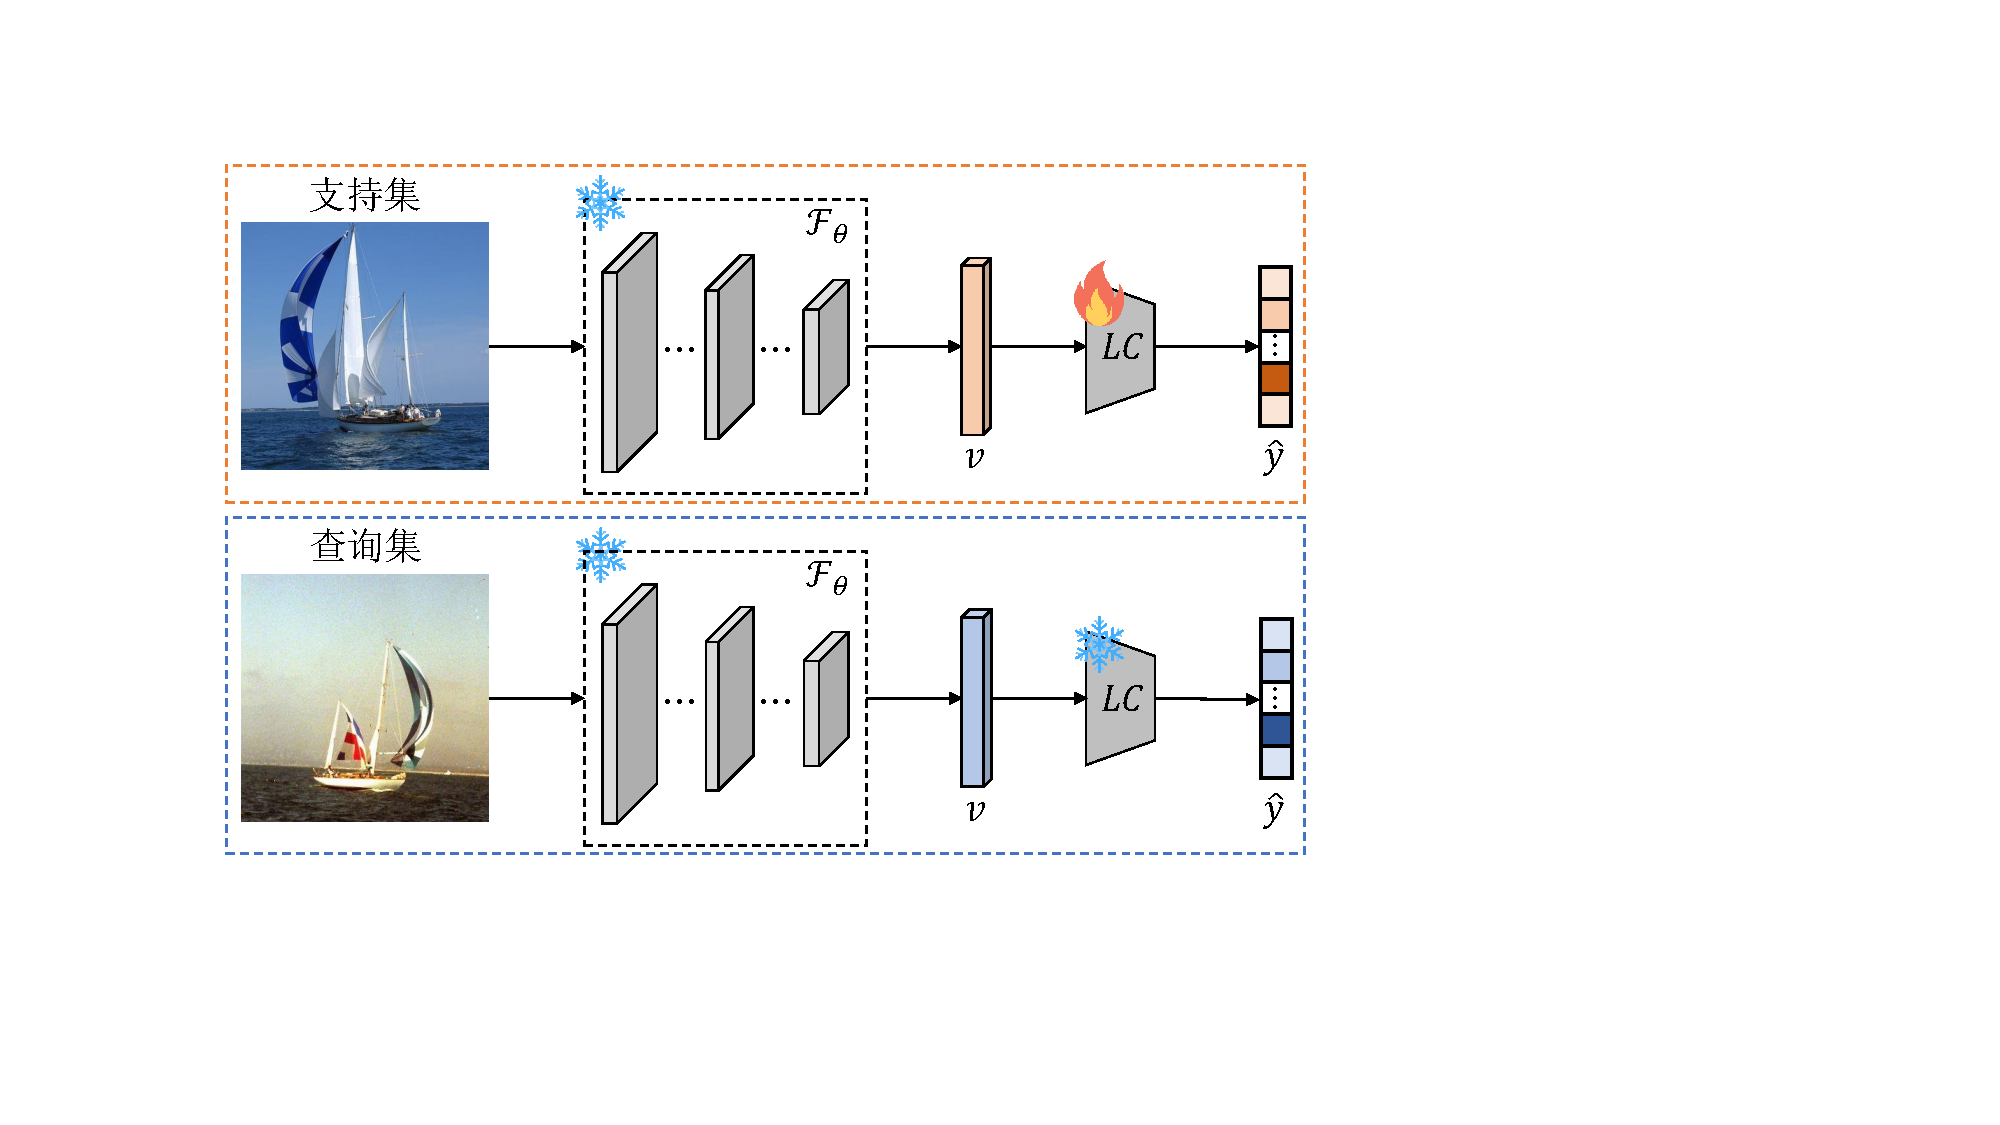
\includegraphics[width=0.8\columnwidth]{figures/MGSRCL/推理过程.pdf}
% \captionsetup{justification=justified,singlelinecheck=false}
\bicaption[MGSRCL模型推理过程示意图]{MGSRCL模型推理过程示意图。推理过程中,使用冻结参数的特征提取网络$\mathcal{F}_{\theta}$提取支持集与查询集的图像特征。其中,支持集特征被用来训练一个逻辑回归分类器$LC$,查询集特征则是用来测试分类器性能。}[Illustration of MGSRCL model inference process]{Illustration of MGSRCL model inference process. During the inference process, the feature extraction network $\mathcal{F}_{\theta}$ with frozen parameters is used to extract image features from both support set and query set. Herein, the support set features are utilized to train a logistic regression classifier $LC$, while the query set features are used to assess the classifier's performance.}
\vspace{-10pt}
\label{figure3: 推理过程}
\end{figure}

\section[\hspace{-2pt}实验设置及结果分析]{{\heiti\zihao{-3} \hspace{-8pt}实验设置及结果分析}}\label{section3: 实验设置及结果分析}
在本节中,首先介绍了本章方法的实验设置,包括数据集设置、网络结构、优化设置、数据增强方式,然后分析了基于多粒度样本关系对比学习的少样本特征学习算法实验结果,接下来对模型的多个模块以及超参数进行了消融实验和分析,最后对模型所提取特征进行了可视化分析。

\subsection[\hspace{-2pt}实验设置]{{\heiti\zihao{4} \hspace{-8pt}实验设置}}\label{section3: 实验设置}

\textbf{(1)实验数据集介绍}

本文在四个常用的少样本分类基准数据集上进行了实验,其中包括三个普通少样本分类数据集:miniImageNet \cite{vinyals2016matching}、tieredImageNet \cite{ren2018meta}、CIFAR-FS \cite{bertinetto2018meta},以及一个细粒度数据集:CUB-200-2011(CUB)\cite{wah2011caltech}。对于所有数据集,本文保持了与其他工作\cite{RFS, RENet, IER}相同的划分准则。在实验中,对于miniImageNet、tieredImageNet和CUB,图像大小为84$\times$84,而对于CIFAR-FS,图像大小为32$\times$32。

\textbf{(2)网络结构}

遵循先前的研究工作\cite{RFS, DeepEMD, IER},本文采用了ResNet-12作为特征提取网络。变换一致性学习(TCL)在标签输出上进行,而类对比学习(CCL)在经过全局池化层后的特征上进行,这些技术不需要额外的网络层。此外,本文添加了一个自监督学习模块,该模块是一个由两个全连接层、一个批归一化层和一个激活函数组成的多层感知机。

\textbf{(3)优化设置}

在所有实验中,本文使用了具有0.9动量和$5e^{-4}$权重衰减的随机梯度下降(Stochastic Gradient Descent,简称SGD)优化器。初始学习率设定为0.05,随后在特定轮次以0.1的倍数衰减。对于tieredImageNet,总共训练了60个轮次,学习率分别在第30、40和50轮次后衰减。对于其他数据集,训练了80个轮次,学习率在第60和70轮次后衰减。关于超参数,本文对所有数据集设置为以下值:$\alpha=1.0$,$\beta=0.1$,$\tau_1=4.0$,$\tau_2=0.1$。

\textbf{(4)数据增强}

为了缓解过拟合问题并进行MGSRCL模型中的变换一致性学习(TCL),本文在训练特征提取网络时添加了一些数据增强样本。数据增强包括三种长宽比例不同的裁剪缩放变换、三种旋转变换(分别为90°、180°和270°)、一种随机擦除、一种图像灰度化和一种Sobel边缘检测。在训练过程中,这些数据增强样本与原始样本一同作为模型的输入。

\subsection[\hspace{-2pt}基准数据集实验结果]{{\heiti\zihao{4} \hspace{-8pt}基准数据集实验结果}}\label{section3: 基准数据集实验结果}

为了评估方法的有效性,本文在四个数据集上进行了广泛的实验。表\ref{table3: mini}、\ref{table3: tiered}、\ref{table3: CIFAR-FS}和\ref{table3: CUB}分别展示了miniImageNet、tieredImageNet、CIFAR-FS和CUB数据集上一些现有少样本分类方法和本文方法的实验结果。此外,本文还将所提模型作为预训练网络结合到三个两阶段少样本分类算法中,并与原方法性能进行对比以进一步验证本文所获得特征提取网络的有效性。


\textbf{(1)普通少样本分类}

如表\ref{table3: mini}和\ref{table3: tiered}所示,本文方法MGSRCL在miniImageNet和tieredImageNet数据集上与其他方法相比取得了出色的性能。具体而言,MGSRCL在miniImageNet上的1-shot和5-shot任务中分别达到了69.57\%和84.41\%的准确率,在tieredImageNet上分别达到了72.98\%和86.23\%的准确率。特别是在5-way 1-shot任务中,MGSRCL达到了最优实验结果,在两个数据集上分别比次优结果高0.20\%和0.30\%。在CIFAR-FS数据集上,MGSRCL在1-shot和5-shot少样本分类任务中分别达到了78.54\%和88.64\%的准确率,在1-shot任务上比次优的PAL方法高1.44\%,如表\ref{table3: CIFAR-FS}所示。值得注意的是,与采用知识蒸馏技术的RFS\cite{RFS}、PAL\cite{PAL}和SCL\cite{Spatial},以及使用元学习方法的DeepEMD\cite{DeepEMD}和ESPT\cite{ESPT}不同,MGSRCL无需进行第二次训练或元学习微调阶段。本文方法使得预训练模型能够达到与最先进方法相媲美甚至超越的性能,这证明了所提方法能够增强模型的特征提取能力和泛化能力,从而使得所提取到的新类特征具有更好的判别性。

{\small    % 设置表格字体为5号
\setstretch{1.245}        % 设置具有指定弹力的橡皮长度(原行宽的1.2倍)
\captionsetup{font={small, stretch=1.512}}
\begin{xltabular}{\textwidth}{lCCC}
\bilingualcaption{MGSRCL在miniImageNet数据集上的分类准确率(\%)}{MGSRCL在miniImageNet数据集上的分类准确率(\%)。最优结果用粗体表示,带有“\dag”标记的方法表示结果是使用作者提供代码所实现。}{Classification accuracy (\%) of MGSRCL on miniImageNet. The best results are shown in bold, and methods with the ``\dag'' indicate that the result was implemented using author-supplied code.}
\label{table3: mini} \\
\toprule
方法 & 特征提取网络 & 5-way 1-shot & 5-way 5-shot \\
\midrule
\endfirsthead

\multicolumn{4}{c}{\tablename \thetable{} (续)} \\ % 第一行标题
\multicolumn{4}{c}{Table \thetable{} (continued)} \\ % 第二行标题

\toprule
方法 & 特征提取网络 & 5-way 1-shot & 5-way 5-shot \\
\midrule
\endhead

% \midrule \multicolumn{3}{r}{{接下页}} \\ 
\bottomrule
\endfoot

\bottomrule
\endlastfoot

% 添加你的内容
MAML \cite{MAML} & 32-32-32-32 & 48.70 $\pm$ 1.84 & 63.11 $\pm$ 0.92 \\
ProtoNet \cite{ProtoNet} & 64-64-64-64 & $ 49.42 \pm 0.78 $ & 68.20 $\pm$ 0.66 \\
DeepEMD \cite{DeepEMD} & ResNet-12 & 65.91 $\pm$ 0.82 & 82.41 $\pm$ 0.56 \\
RFS-distill \cite{RFS} & ResNet-12 & 64.82 $\pm$ 0.60 & 82.14 $\pm$ 0.43 \\
AssoAlign \cite{AssoAlign} & ResNet-18 & 59.88 $\pm$ 0.67 & 80.35 $\pm$ 0.73 \\
GIFSL \cite{GIFSL} & ResNet-12 & 65.47 $\pm$ 0.63 & 82.75 $\pm$ 0.42 \\
MELR \cite{MELR} & ResNet-12 & 67.40 $\pm$ 0.43 & 83.40 $\pm$ 0.28\\
IEPT \cite{IEPT} & ResNet-12 & 67.05 $\pm$ 0.44 & 82.90 $\pm$ 0.30 \\
IER \cite{IER} & ResNet-12 & 66.82 $\pm$ 0.80 & 84.35 $\pm$ 0.51 \\
RENet \cite{RENet} & ResNet-12 & 67.60 $\pm$ 0.44 & 82.58 $\pm$ 0.30 \\
PAL \cite{PAL} & ResNet-12 & 69.37 $\pm$ 0.64 & 84.40 $\pm$ 0.44 \\
HandCrafted \cite{HandCrafted} & ResNet-12 & 67.14 $\pm$ 0.76 & 83.11 $\pm$ 0.69 \\
PDA \cite{PDA} & ResNet-12 & 65.75 $\pm$ 0.43 & 83.37 $\pm$ 0.30 \\
SCL-distill \cite{Spatial} & ResNet-12 & 67.40 $\pm$ 0.76 & 83.19 $\pm$ 0.54 \\
HGNN \cite{HGNN} & ResNet-12 & 67.02 $\pm$ 0.20 & 83.00 $\pm$ 0.13 \\
APP2S \cite{APP2S} & ResNet-18 & 64.82 $\pm$ 0.12 & 81.31 $\pm$ 0.22 \\
DGAP \cite{DGAP} & ResNet-12 & 61.35 $\pm$ 0.62 & 78.85 $\pm$ 0.46 \\
ESPT \cite{ESPT} & ResNet-12 & 68.36 $\pm$ 0.19 & 84.11 $\pm$ 0.12 \\
Meta-HP \cite{Meta-HP} & ResNet-12 & 62.49 $\pm$ 0.80 & 77.12 $\pm$ 0.62 \\
SAPENet \cite{SAPENet} & ResNet-12 & 66.41 $\pm$ 0.20 & 82.76 $\pm$ 0.14 \\
FEAT+DFR \cite{DFR} & ResNet-12 & 67.74 $\pm$ 0.86 & 82.49 $\pm$ 0.57 \\
DiffKendall \cite{DiffKendall} & ResNet-12 & 65.56 $\pm$ 0.43 & 80.79 $\pm$ 0.31 \\
\midrule
FEAT \cite{FEAT} & ResNet-12 & 66.78 $\pm$ 0.20 & 82.05 $\pm$ 0.14 \\
\textbf{MGSRCL + FEAT} & ResNet-12 & 69.27 $\pm$ 0.21 & 83.59 $\pm$ 0.13 \\
\midrule
Meta-Baseline\dag \cite{MetaBaseline} & ResNet-12 & 63.38 $\pm$ 0.23 & 79.48 $\pm$ 0.16 \\
\textbf{MGSRCL + Meta-Baseline} & ResNet-12 & 69.01 $\pm$ 0.23 & 83.94 $\pm$ 0.15 \\
\midrule
STVAE \cite{STVAE} & ResNet-12 & 63.62 $\pm$ 0.80 & 80.68 $\pm$ 0.48 \\
\textbf{MGSRCL + STVAE} & ResNet-12 & 67.29 $\pm$ 0.89 & 82.62 $\pm$ 0.58 \\
\midrule
\textbf{MGSRCL} & ResNet-12 & \textbf{69.57 $\pm$ 0.45} & \textbf{84.41 $\pm$ 0.30} \\
\end{xltabular}}


{
\small    % 设置表格字体为5号
\setstretch{1.245}        % 设置具有指定弹力的橡皮长度(原行宽的1.2倍)
\captionsetup{font={small, stretch=1.512}}
\begin{xltabular}{\textwidth}{lCCC}
\bilingualcaption{MGSRCL在tieredImageNet数据集上的分类准确率(\%)}{MGSRCL在tieredImageNet数据集上的分类准确率(\%)。最优结果用粗体表示,带有“\dag”标记的方法表示结果是使用作者提供代码所实现。}{Classification accuracy (\%) of MGSRCL on tieredImageNet. The best results are shown in bold, and methods with the ``\dag'' indicate that the result was implemented using author-supplied code.}
\label{table3: tiered} \\
\toprule
方法 & 特征提取网络 & 5-way 1-shot & 5-way 5-shot \\
\midrule
\endfirsthead

\multicolumn{4}{c}{\tablename \thetable{} (续)} \\ % 第一行标题
\multicolumn{4}{c}{Table \thetable{} (continued)} \\ % 第二行标题

\toprule
方法 & 特征提取网络 & 5-way 1-shot & 5-way 5-shot \\
\midrule
\endhead

% \midrule \multicolumn{3}{r}{{接下页}} \\ 
\bottomrule
\endfoot

\bottomrule
\endlastfoot

% 添加你的内容
MAML \cite{MAML} & 32-32-32-32 & 51.67 $\pm$ 1.81 & 70.30 $\pm$ 1.75 \\
ProtoNet \cite{ProtoNet} & 64-64-64-64  & 53.31 $\pm$ 0.89 & 72.69 $\pm$ 0.74 \\
DeepEMD \cite{DeepEMD} & ResNet-12 & 71.16 $\pm$ 0.87 & 86.03 $\pm$ 0.58 \\
RFS-distill \cite{RFS} & ResNet-12 & 71.52 $\pm$ 0.69 & 86.03 $\pm$ 0.49 \\
AssoAlign \cite{AssoAlign} & ResNet-18 & 69.29 $\pm$ 0.56 & 85.97 $\pm$ 0.49 \\
GIFSL \cite{GIFSL} & ResNet-12 & 72.39 $\pm$ 0.66 & 86.91 $\pm$ 0.44 \\
MELR \cite{MELR} & ResNet-12 & 72.14 $\pm$ 0.51 & 87.01 $\pm$ 0.35 \\
IEPT \cite{IEPT} & ResNet-12 & 72.24 $\pm$ 0.50 & 86.73 $\pm$ 0.34 \\
IER \cite{IER} & ResNet-12 & 71.87 $\pm$ 0.89 & 86.82 $\pm$ 0.58 \\
RENet \cite{RENet} & ResNet-12 & 71.16 $\pm$ 0.51 & 85.28 $\pm$ 0.35 \\
PAL \cite{PAL} & ResNet-12 & 72.25 $\pm$ 0.72 & 86.95 $\pm$ 0.47 \\
PDA \cite{PDA} & ResNet-12 & 72.28 $\pm$ 0.49 & 86.70 $\pm$ 0.33 \\
SCL-distill \cite{Spatial} & ResNet-12 & 71.98 $\pm$ 0.91 & 86.19 $\pm$ 0.59 \\
HGNN \cite{HGNN} & ResNet-12 & 72.05 $\pm$ 0.23 & 86.49 $\pm$ 0.15 \\
APP2S \cite{APP2S} & ResNet-18 & 70.83 $\pm$ 0.15 & 84.15 $\pm$ 0.29 \\
DGAP \cite{DGAP} & ResNet-12 & 70.10 $\pm$ 0.67 & 84.99 $\pm$ 0.46 \\
ESPT \cite{ESPT} & ResNet-12 & 72.68 $\pm$ 0.22 & \textbf{87.49 $\pm$ 0.14} \\
Meta-HP \cite{Meta-HP} & ResNet-12 & 68.26 $\pm$ 0.72 & 82.91 $\pm$ 0.36 \\
SAPENet \cite{SAPENet} & ResNet-12 & 68.63 $\pm$ 0.23 & 84.30 $\pm$ 0.16 \\
FEAT+DFR \cite{DFR} & ResNet-12 & 71.31 $\pm$ 0.93 & 85.12 $\pm$ 0.64 \\
DiffKendall \cite{DiffKendall} & ResNet-12 & 70.76 $\pm$ 0.43 & 85.31 $\pm$ 0.34 \\
\midrule
FEAT \cite{FEAT} & ResNet-12 & 70.80 $\pm$ 0.23 & 84.79 $\pm$ 0.16 \\
\textbf{MGSRCL + FEAT} & ResNet-12 & 72.02 $\pm$ 0.23  & 86.19 $\pm$ 0.15 \\
\midrule
Meta-Baseline\dag \cite{MetaBaseline} & ResNet-12 & 68.74 $\pm$ 0.26 & 83.45 $\pm$ 0.18 \\
\textbf{MGSRCL + Meta-Baseline} & ResNet-12 & 69.79 $\pm$ 0.26 & 83.55 $\pm$ 0.18 \\
\midrule
STVAE\dag \cite{STVAE} & ResNet-12 & 68.32 $\pm$ 0.94 & 83.79 $\pm$ 0.66 \\
\textbf{MGSRCL + STVAE} & ResNet-12 & 72.03 $\pm$ 0.89 & 84.49 $\pm$ 0.66 \\
\midrule
\textbf{MGSRCL} & ResNet-12 & \textbf{72.98 $\pm$ 0.51} & 86.23 $\pm$ 0.34 \\
\end{xltabular}}

{
\small    % 设置表格字体为5号
\setstretch{1.245}        % 设置具有指定弹力的橡皮长度(原行宽的1.2倍)
\captionsetup{font={small, stretch=1.512}}
\begin{xltabular}{\textwidth}{lCCC}
\bilingualcaption{MGSRCL在CIFAR-FS数据集上的分类准确率(\%)}{MGSRCL在CIFAR-FS数据集上的分类准确率(\%)。最优结果用粗体表示,带有“\dag”标记的方法表示结果是使用作者提供代码所实现。}{Classification accuracy (\%) of MGSRCL on CIFAR-FS. The best results are shown in bold, and methods with the ``\dag'' indicate that the result was implemented using author-supplied code.}
\label{table3: CIFAR-FS} \\
\toprule
方法 & 特征提取网络 & 5-way 1-shot & 5-way 5-shot \\
\midrule
\endfirsthead

\multicolumn{4}{c}{\tablename \thetable{} (续)} \\ % 第一行标题
\multicolumn{4}{c}{Table \thetable{} (continued)} \\ % 第二行标题

\toprule
方法 & 特征提取网络 & 5-way 1-shot & 5-way 5-shot \\
\midrule
\endhead

% \midrule \multicolumn{3}{r}{{接下页}} \\ 
\bottomrule
\endfoot

\bottomrule
\endlastfoot

% 添加你的内容
MAML \cite{MAML} & 32-32-32-32 & 58.90 $\pm$ 1.90 & 71.50 $\pm$ 1.00 \\
ProtoNet \cite{ProtoNet} & 64-64-64-64 & 55.50 $\pm$ 0.70 & 72.00 $\pm$ 0.60 \\
RFS-distill \cite{RFS} & ResNet-12 & 73.90 $\pm$ 0.80 & 86.90 $\pm$ 0.50  \\
GIFSL \cite{GIFSL} & ResNet-12 & 74.58 $\pm$ 0.38 & 87.68 $\pm$ 0.23 \\
IER \cite{IER} & ResNet-12 & 76.83 $\pm$ 0.82 & 89.26 $\pm$ 0.58  \\
RENet \cite{RENet} & ResNet-12 & 74.51 $\pm$ 0.46 & 86.60 $\pm$ 0.32  \\
PAL \cite{PAL} & ResNet-12 & 77.10 $\pm$ 0.70 & 88.00 $\pm$ 0.50  \\
HandCrafted \cite{HandCrafted} & ResNet-12 & 76.68 $\pm$ 0.59 & 87.49 $\pm$ 0.73 \\
SCL-distill \cite{Spatial} & ResNet-12 & 76.50 $\pm$ 0.90 & 88.00 $\pm$ 0.60  \\
ConstellationNet \cite{ConstellationNet} & ResNet-12 & 75.40 $\pm$ 0.20 & 86.80 $\pm$ 0.20  \\
APP2S \cite{APP2S} & ResNet-18 & 73.12 $\pm$ 0.22 & 85.69 $\pm$ 0.16 \\
Meta-HP \cite{Meta-HP} & ResNet-12 & 73.74 $\pm$ 0.57 & 86.37 $\pm$ 0.32 \\
\midrule
FEAT\dag \cite{FEAT} & ResNet-12 & 75.97 $\pm$ 0.21 & 87.34 $\pm$ 0.14 \\
\textbf{MGSRCL + FEAT} & ResNet-12 & 79.91 $\pm$ 0.21 & \textbf{90.18 $\pm$ 0.14} \\
\midrule
Meta-Baseline\dag \cite{MetaBaseline} & ResNet-12 & 74.56 $\pm$ 0.39 & 86.24 $\pm$ 0.27 \\
\textbf{MGSRCL + Meta-Baseline} & ResNet-12 & 78.51 $\pm$ 0.24 & 88.60 $\pm$ 0.16 \\
\midrule
STVAE \cite{STVAE} & ResNet-12 & 76.30 $\pm$ 0.60 & 87.00 $\pm$ 0.40 \\
\textbf{MGSRCL + STVAE} & ResNet-12 & \textbf{80.92 $\pm$ 0.72} & 86.38 $\pm$ 0.60 \\
\midrule
\textbf{MGSRCL} & ResNet-12 & 78.54 $\pm$ 0.47 & 88.64 $\pm$ 0.32 \\
\end{xltabular}}


\textbf{(2)细粒度少样本分类}

为了进一步验证所提方法的泛化能力,本文还在一个细粒度少样本分类数据集(CUB)上对所提的MGSRCL方法进行了实验,实验结果如表\ref{table3: CUB}所示。本文方法在1-shot和5-shot任务中都取得了最优结果,分别达到了86.14\%和94.75\%的分类准确率,比次优结果高出0.69\%和0.02\%。这些结果表明,在不同类别之间差异微小的细粒度数据集上,本文方法通过探索不同粒度的样本关系并对它们进行细致建模,能够更好地区分细粒度类别,进一步证明了方法的有效性。

{
\small    % 设置表格字体为5号
\setstretch{1.245}        % 设置具有指定弹力的橡皮长度(原行宽的1.2倍)
\captionsetup{font={small, stretch=1.512}}
\begin{xltabular}{\textwidth}{lCCC}
\bilingualcaption{MGSRCL在CUB数据集上的分类准确率(\%)}{MGSRCL在CUB数据集上的分类准确率(\%)。最优结果用粗体表示,带有“\dag”标记的方法表示结果是使用作者提供代码所实现。}{Classification accuracy (\%) of MGSRCL on CUB. The best results are shown in bold, and methods with the ``\dag'' indicate that the result was implemented using author-supplied code.}
\label{table3: CUB} \\
\toprule
方法 & 特征提取网络 & 5-way 1-shot & 5-way 5-shot \\
\midrule
\endfirsthead

\multicolumn{4}{c}{\tablename \thetable{} (续)} \\ % 第一行标题
\multicolumn{4}{c}{Table \thetable{} (continued)} \\ % 第二行标题

\toprule
方法 & 特征提取网络 & 5-way 1-shot & 5-way 5-shot \\
\midrule
\endhead

% \midrule \multicolumn{3}{r}{{接下页}} \\ 
\bottomrule
\endfoot

\bottomrule
\endlastfoot

% 添加你的内容
FEAT \cite{FEAT} & 64-64-64-64 & 68.87 $\pm$ 0.22 & 82.90 $\pm$ 0.15 \\
DeepEMD \cite{DeepEMD} & ResNet-12 & 75.65 $\pm$ 0.83 & 88.69 $\pm$ 0.50 \\
AssoAlign \cite{AssoAlign} & ResNet-18 & 74.22 $\pm$ 1.09 & 88.65 $\pm$ 0.55 \\
MELR \cite{MELR} & 64-64-64-64 & 70.26 $\pm$ 0.50 & 85.01 $\pm$ 0.32 \\
IEPT \cite{IEPT} & 64-64-64-64 & 69.97 $\pm$ 0.49 & 84.33 $\pm$ 0.33 \\
RENet \cite{RENet} & ResNet-12 & 79.49 $\pm$ 0.44 & 91.11 $\pm$ 0.24 \\
HGNN \cite{HGNN} & ResNet-12 & 78.58 $\pm$ 0.20 & 90.02 $\pm$ 0.12 \\
APP2S \cite{APP2S} & ResNet-12 & 77.64 $\pm$ 0.19 & 90.43 $\pm$ 0.18 \\
ESPT \cite{ESPT} & ResNet-12 & 85.45 $\pm$ 0.18 & 94.02 $\pm$ 0.09 \\
SAPENet \cite{SAPENet} & 64-64-64-64 & 70.38 $\pm$ 0.23 & 84.47 $\pm$ 0.14 \\
FEAT+DFR \cite{DFR} & ResNet-12 & 77.14 $\pm$ 0.21 & 88.97 $\pm$ 0.13 \\
Bi-FRN \cite{Bi-FRN} & ResNet-12 & 85.44 $\pm$ 0.18 & 94.73 $\pm$ 0.09 \\
\midrule
FEAT\dag \cite{FEAT} & ResNet-12 & 77.60 $\pm$ 0.45 & 89.20 $\pm$ 0.28 \\
\textbf{MGSRCL + FEAT} & ResNet-12 & 84.23 $\pm$ 0.19 & 92.67 $\pm$ 0.10 \\
\midrule
Meta-Baseline\dag \cite{MetaBaseline} & ResNet-12 & 75.04 $\pm$ 0.24 & 87.57 $\pm$ 0.14 \\
\textbf{MGSRCL + Meta-Baseline} & ResNet-12 & \textbf{88.37 $\pm$ 0.18} & \textbf{95.52 $\pm$ 0.09} \\
\midrule
STVAE \cite{STVAE} & ResNet-12 & 77.32 $\pm$ 0.00 & 86.84 $\pm$ 0.00 \\
\textbf{MGSRCL + STVAE} & ResNet-12 & 84.35 $\pm$ 0.76 & 93.69 $\pm$ 0.39 \\
\midrule
\textbf{MGSRCL} & ResNet-12 & 86.14 $\pm$ 0.38 & 94.75 $\pm$ 0.19 \\
\end{xltabular}}


\textbf{(3)与其他方法结合}

此外,作为一种基于特征学习的方法,本文方法可以为两阶段元学习方法和一些生成方法提供一个良好的预训练模型,帮助它们实现更好的性能。为了证明这一点,本文选择了两种元学习方法(FEAT\cite{FEAT}、Meta-Baseline\cite{MetaBaseline})和一种生成方法(STVAE\cite{STVAE}),在四个数据集上进行了实验。因为这些方法的特征提取网络与本文存在一些差异,或者它们没有在相应数据集上进行实验,本文对一些方法根据原作者提供代码进行了重新实现,实验结果以“\dag”进行标记。如表\ref{table3: mini}和\ref{table3: tiered}所示,当使用本文的预训练模型时,FEAT、Meta-Baseline和STVAE在miniImageNet数据集的1-shot任务中的分类准确率分别提高了2.49\%、5.63\%和3.67\%,在5-shot任务中分别提高了1.54\%、4.46\%和1.94\%。FEAT、Meta-Baseline和STVAE在使用本文模型作为预训练模型时,在tieredImageNet数据集上的性能也同样有所提升。在CIFAR-FS数据集上,使用本文预训练模型的STVAE和FEAT在1-shot和5-shot任务中分别取得了最优结果,准确率分别为80.92\%和90.18\%,如表\ref{table3: CIFAR-FS}所示。进一步地,本文还在CUB数据集上对这些方法进行了实验,其中Meta-Baseline在1-shot和5-shot少样本分类任务中表现突出,分别达到了88.37\%和95.52\%的准确率,如表\ref{table3: CUB}所示。这些实验结果表明,本文方法可以为这些两阶段元学习方法和生成方法提供一个优质的预训练模型,以提高它们的性能,也再一次验证了特征提取网络对少样本分类问题的重要性。

\begin{table}[h!]
\small    % 设置表格字体为5号
\setstretch{1.245}        % 设置具有指定弹力的橡皮长度(原行宽的1.2倍)
\captionsetup{font={small, stretch=1.512}}
\centering
% \vspace{-10pt}
% \captionsetup{justification=justified,singlelinecheck=false}
\bicaption[MGSRCL在miniImageNet、CIFAR-FS和CUB数据集上的模块消融实验]{MGSRCL在miniImageNet、CIFAR-FS和CUB数据集上的模块消融实验。最优结果用粗体表示。}[Module ablation experiments of MGSRCL on miniImageNet, CIFAR-FS and CUB]{Module ablation experiments of MGSRCL on miniImageNet, CIFAR-FS and CUB. The best results are shown in bold.}    % 中英文标题
\begin{tabularx}{\textwidth}{ClCC}
\toprule
数据集 & 方法 & 5-way 1-shot & 5-way 5-shot \\
\midrule
\multirow{6}{*}{miniImageNet}
& Baseline & 66.78 $\pm$ 0.43 & 83.82 $\pm$ 0.29 \\
& Baseline w/ SS &  67.76 $\pm$ 0.44 & 84.31 $\pm$ 0.28 \\
& Baseline w/ TCL & 68.45 $\pm$ 0.44 & 84.37 $\pm$ 0.29 \\
& Baseline w/ CCL & 68.61 $\pm$ 0.44 & 84.13 $\pm$ 0.29 \\
& Baseline w/ TCL \& CCL & 69.21 $\pm$ 0.45 & 84.37 $\pm$ 0.30 \\
& Baseline w/ all & \textbf{69.57 $\pm$ 0.45} & \textbf{84.41 $\pm$ 0.30} \\
\midrule
\multirow{6}{*}{CIFAR-FS}
& Baseline & 74.39 $\pm$ 0.46 & 88.10 $\pm$ 0.33 \\
& Baseline w/ SS & 76.42 $\pm$ 0.45 & 88.62 $\pm$ 0.32 \\
& Baseline w/ TCL & 77.65 $\pm$ 0.47 & 88.51 $\pm$ 0.32 \\
& Baseline w/ CCL & 77.61 $\pm$ 0.47 & 88.59 $\pm$ 0.32 \\
& Baseline w/ TCL \& CCL & 78.01 $\pm$ 0.48 & 88.27 $\pm$ 0.33 \\
& Baseline w/ all & \textbf{78.54 $\pm$ 0.47} & \textbf{88.64 $\pm$ 0.32} \\
\midrule
\multirow{6}{*}{CUB}
& Baseline & 82.18 $\pm$ 0.40 & 93.70 $\pm$ 0.20 \\
& Baseline w/ SS & 83.46 $\pm$ 0.39 & 94.18 $\pm$ 0.20 \\
& Baseline w/ TCL & 83.16 $\pm$ 0.39 & 93.74 $\pm$ 0.20 \\
& Baseline w/ CCL & 85.30 $\pm$ 0.38 & 94.50 $\pm$ 0.19 \\
& Baseline w/ TCL \& CCL & 85.53 $\pm$ 0.38 & 94.30 $\pm$ 0.19 \\
& Baseline w/ all & \textbf{86.14 $\pm$ 0.38} & \textbf{94.75 $\pm$ 0.19} \\
\bottomrule
\end{tabularx}
% \vspace{-25pt}
\label{table3: module ablation}
\end{table}


\subsection[\hspace{-2pt}消融实验]{{\heiti\zihao{4} \hspace{-8pt}消融实验}}\label{section3: 消融实验}

\textbf{(1)讨论不同模块对模型性能的影响}

为了研究MGSRCL模型中每个模块对模型性能的影响,本文在miniImageNet、CIFAR-FS和CUB三个数据集上进行了全面的消融实验。本文的基准模型(Baseline)与RFS\cite{RFS}相同,但为了缓解过拟合问题并实施变换一致性学习(TCL),本文添加了一些数据增强样本。

如表\ref{table3: module ablation}所示,本文的基准模型在miniImageNet、CIFAR-FS和CUB的5-way 1-shot少样本分类任务中分别达到了66.78\%、74.39\%和82.18\%的准确率。当添加自监督模块以预测执行了哪种图像变换时,在三个数据集上相较于基准模型分别获得了0.98\%、2.03\%和1.28\%的效果提升。通过约束同一样本在不同变换下的样本内关系(在基准模型上添加TCL模块),在三个数据集上分别获得了1.67\%、3.26\%和0.98\%的效果提升。通过约束同类样本的类内关系和不同类样本的类间关系(在基准模型上添加CCL模块),在三个数据集上相较于基准模型分别获得了1.83\%、3.22\%和3.12\%的效果提升。此外,对于5-way 5-shot少样本分类任务,添加不同模块也使得模型取得了优于或与基准模型相当的结果。在CUB数据集上,添加CCL模块的结果明显优于添加其他模块,这是因为CUB是一个细粒度数据集,不同类别之间的差异相对较小,将不同类别在特征空间进行推远在CUB数据集上比在miniImageNet和CIFAR-FS数据集上更加有效。

此外,联合使用TCL和CCL模块时,本文模型在5-way 1-shot任务中的结果优于仅使用其中一个模块,分类准确率在miniImageNet、CIFAR-FS和CUB数据集上分别达到了69.21\%、78.01\%和85.53\%的准确率。当使用所有三个模块(TCL、CCL和SS)时,本文模型在三个数据集上都取得了最优性能,分别为69.57\%、78.54\%和86.14\%的1-shot任务准确率,以及84.41\%、88.64\%和94.75\%的5-shot任务准确率。综上所述,这些实验结果证明了本文方法每个模块的作用,以及所提出的TCL模块和CCL模块对挖掘不同粒度样本关系的有效性。

\textbf{(2)讨论超参数$\alpha$和$\beta$对模型性能的影响}

$\alpha$和$\beta$是用来调整不同损失权重的超参数。本文通过将$\alpha$和$\beta$设置为不同数值来评估模型在miniImageNet、CIFAR-FS和CUB数据集上的性能,从而确定其最优值。

\begin{figure}[h!]
\centering
\captionsetup{font={small, stretch=1.312}}
\begin{subfigure}{0.495\columnwidth}
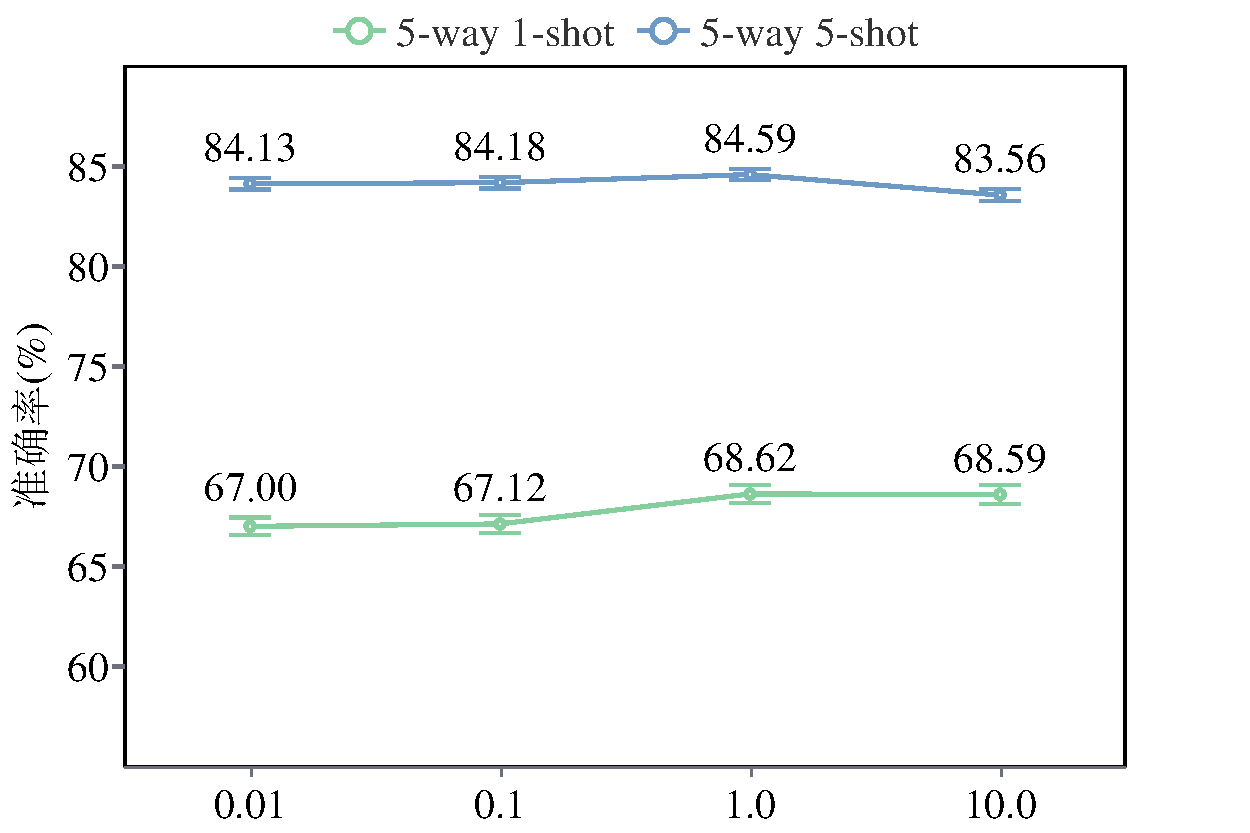
\includegraphics[width=\columnwidth]{figures/MGSRCL/miniImageNet/alpha.pdf}
\caption{$\alpha$}
\label{figure3: alpha(mini)}
\end{subfigure}
\begin{subfigure}{0.495\columnwidth}
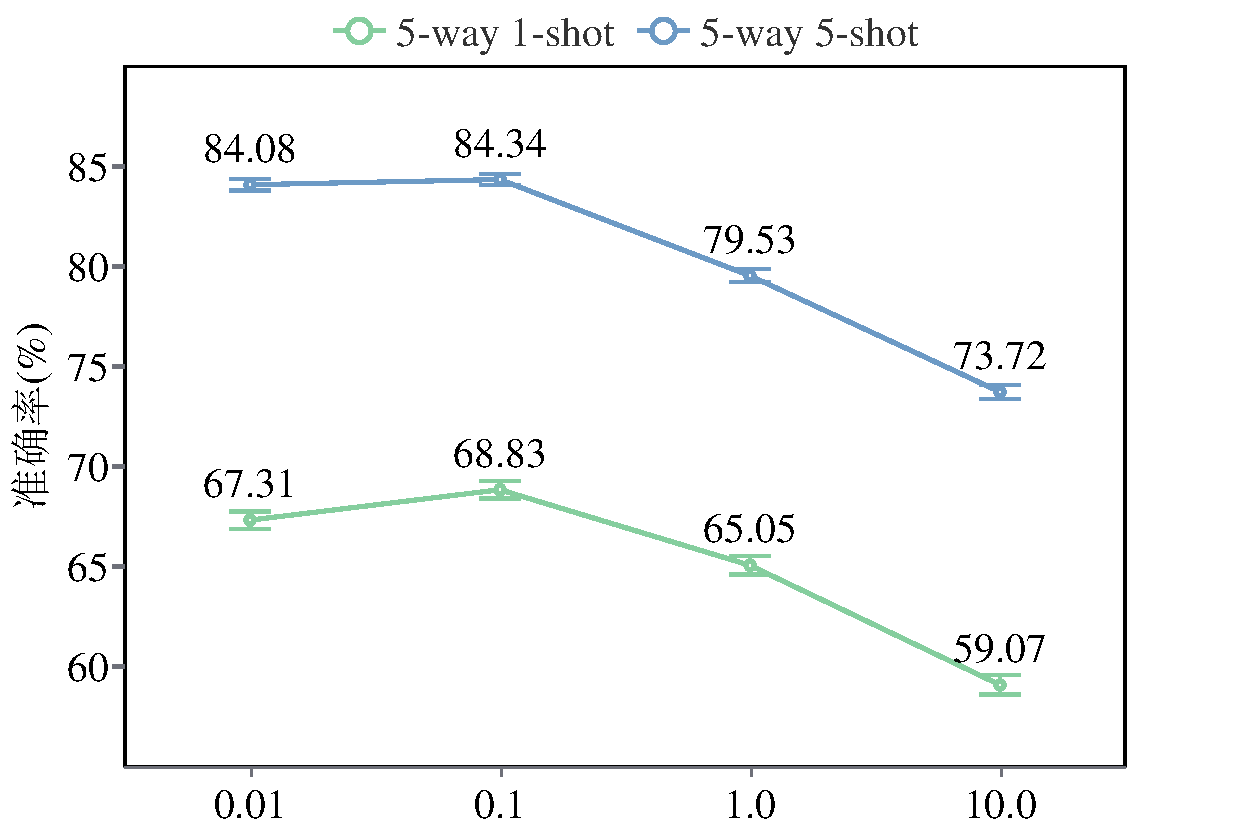
\includegraphics[width=\columnwidth]{figures/MGSRCL/miniImageNet/beta.pdf}
\caption{$\beta$}
\label{figure3: beta(mini)}
\end{subfigure}
\bicaption[MGSRCL在miniImageNet数据集上的超参数$\alpha$和$\beta$消融实验]{MGSRCL在miniImageNet数据集上的超参数$\alpha$和$\beta$消融实验。}[Hyperparameters $\alpha$ and $\beta$ ablation experiments of MGSRCL on miniImageNet]{Hyperparameters $\alpha$ and $\beta$ ablation experiments of MGSRCL on miniImageNet.}
\label{figure3: alpha and beta (mini)}
% \vspace{-4pt}
\end{figure}

\begin{figure}[h!]
\centering
\captionsetup{font={small, stretch=1.312}}
\begin{subfigure}{0.495\columnwidth}
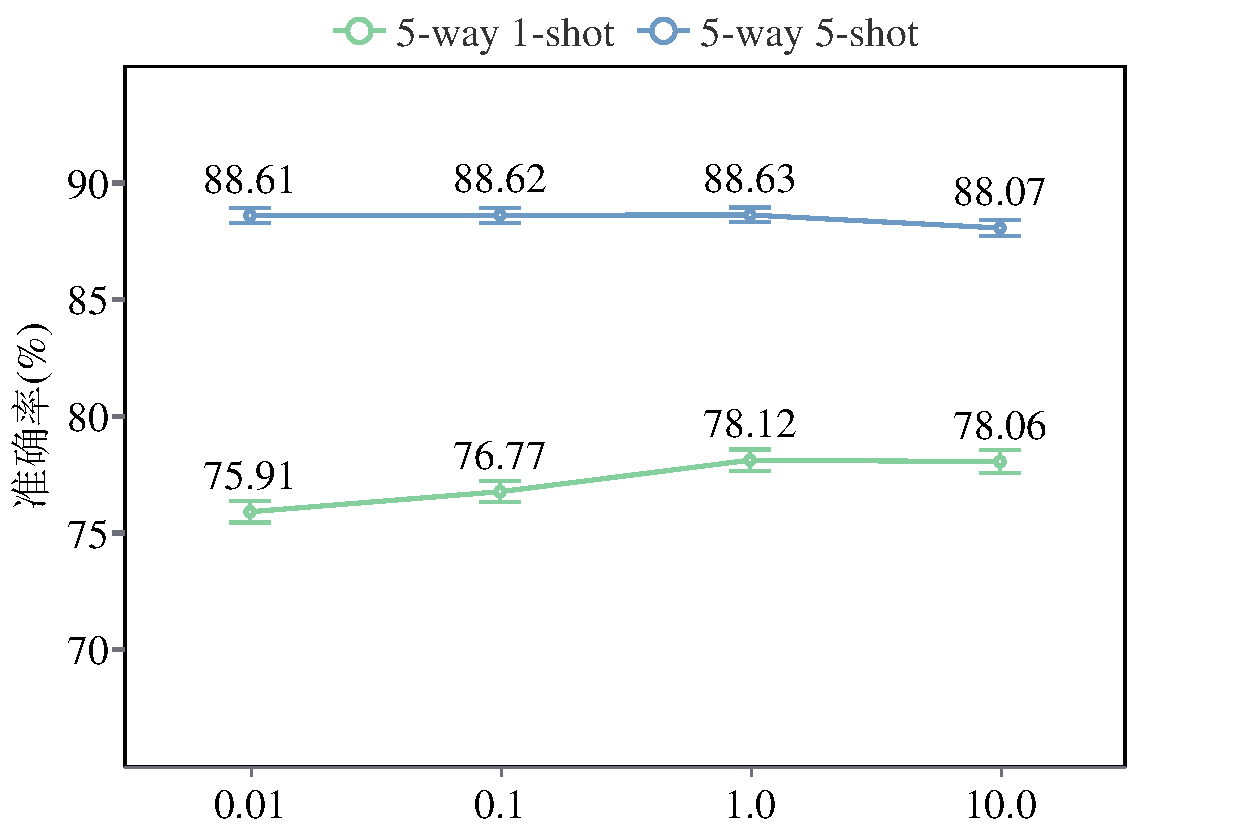
\includegraphics[width=\columnwidth]{figures/MGSRCL/CIFAR-FS/alpha.pdf}
\caption{$\alpha$}
\label{figure3: alpha(CIFAR-FS)}
\end{subfigure}
\begin{subfigure}{0.495\columnwidth}
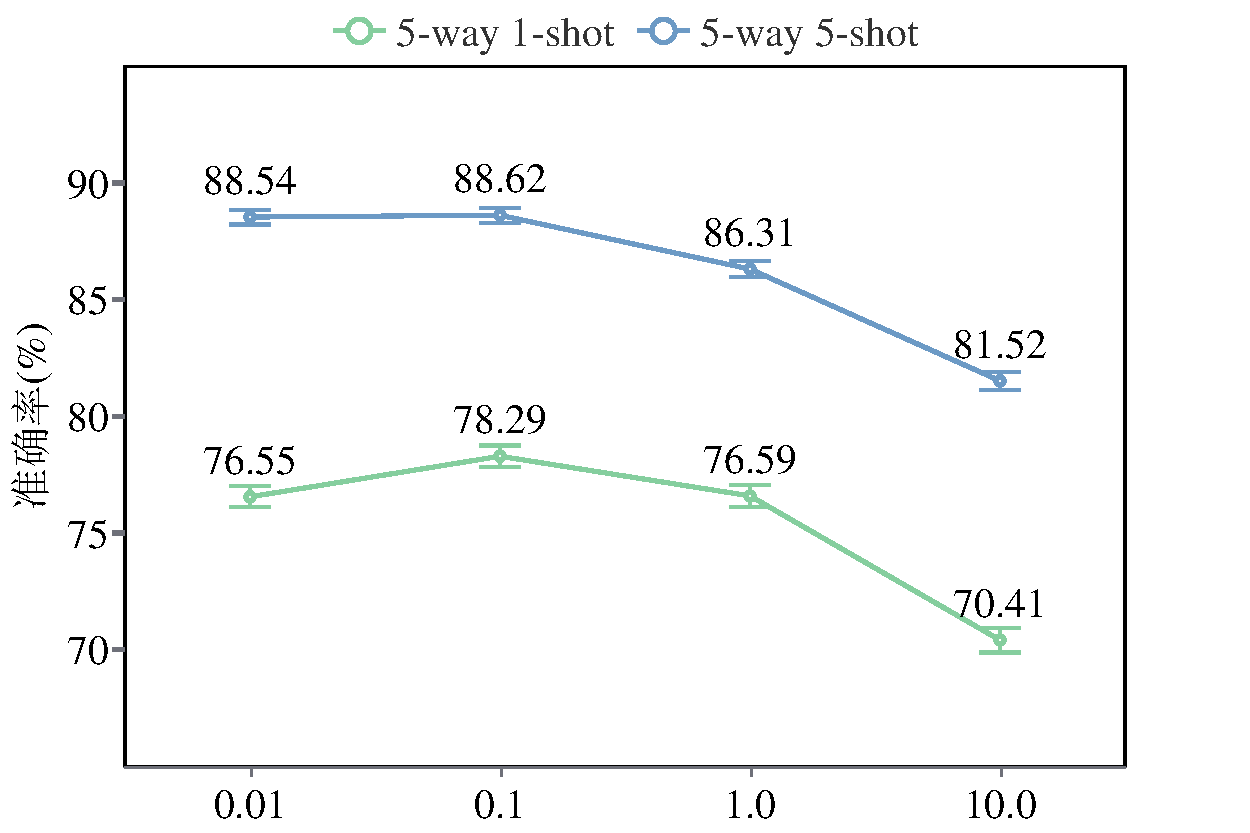
\includegraphics[width=\columnwidth]{figures/MGSRCL/CIFAR-FS/beta.pdf}
\caption{$\beta$}
\label{figure3: beta(CIFAR-FS)}
\end{subfigure}
\bicaption[MGSRCL在CIFAR-FS数据集上的超参数$\alpha$和$\beta$消融实验]{MGSRCL在CIFAR-FS数据集上的超参数$\alpha$和$\beta$消融实验。}[Hyperparameters $\alpha$ and $\beta$ ablation experiments of MGSRCL on CIFAR-FS]{Hyperparameters $\alpha$ and $\beta$ ablation experiments of MGSRCL on CIFAR-FS.}
\label{figure3: alpha and beta (CIFAR-FS)}
% \vspace{-5pt}
\end{figure}

\begin{figure}[h!]
\centering
\captionsetup{font={small, stretch=1.312}}
\begin{subfigure}{0.495\columnwidth}
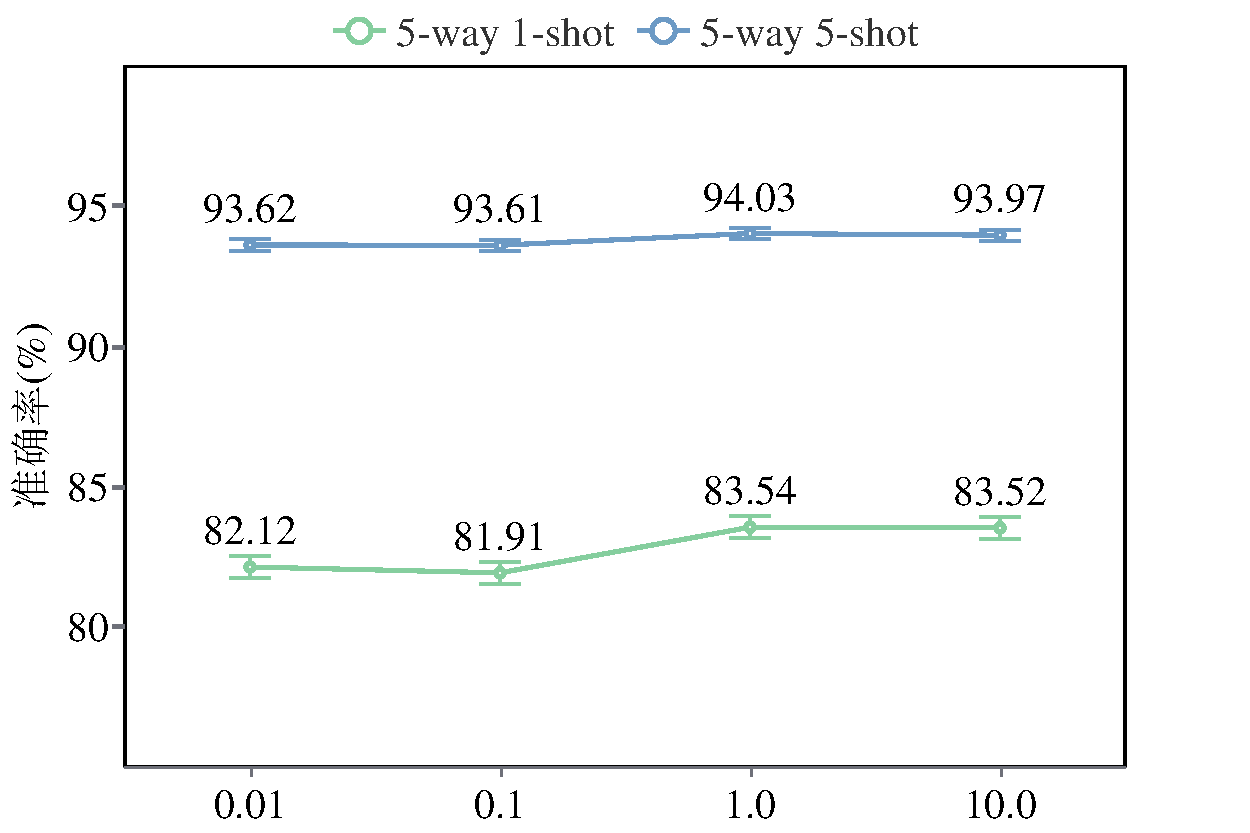
\includegraphics[width=\columnwidth]{figures/MGSRCL/CUB/alpha.pdf}
\caption{$\alpha$}
\label{figure3: alpha(CUB)}
\end{subfigure}
\begin{subfigure}{0.495\columnwidth}
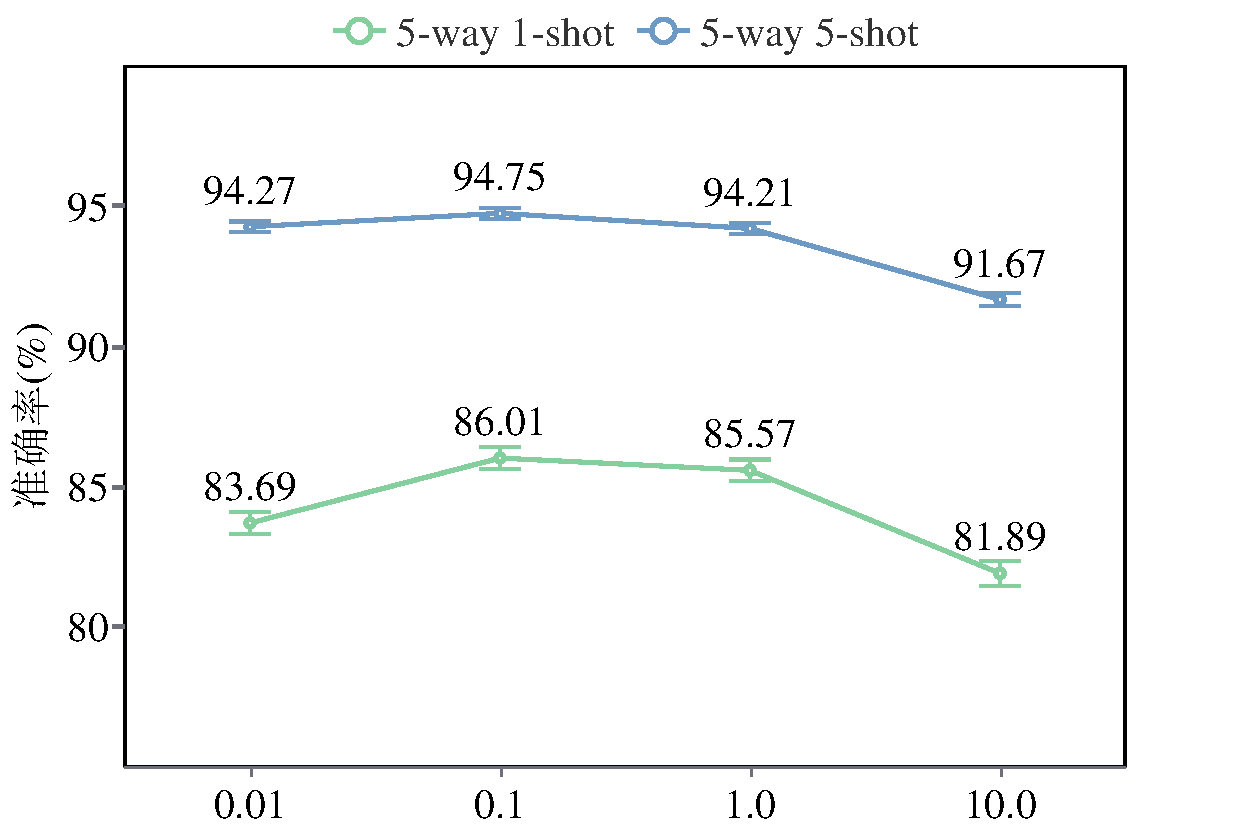
\includegraphics[width=\columnwidth]{figures/MGSRCL/CUB/beta.pdf}
\caption{$\beta$}
\label{figure3: beta(CUB)}
\end{subfigure}
\bicaption[MGSRCL在CUB数据集上的超参数$\alpha$和$\beta$消融实验]{MGSRCL在CUB数据集上的超参数$\alpha$和$\beta$消融实验。}[Hyperparameters $\alpha$ and $\beta$ ablation experiments of MGSRCL on CUB]{Hyperparameters $\alpha$ and $\beta$ ablation experiments of MGSRCL on CUB.}
\label{figure3: alpha and beta (CUB)}
% \vspace{-5pt}
\end{figure}

首先,为了观察模型分类结果随参数变化的趋势,在讨论一个超参数的影响时,本文将另一个超参数设置为0。如图\ref{figure3: alpha and beta (mini)}、\ref{figure3: alpha and beta (CIFAR-FS)}和\ref{figure3: alpha and beta (CUB)}所示,对于超参数$\alpha$,模型性能的变化较为平缓,整体呈现先上升再下降的趋势。当$\alpha = 1.0$时,模型性能在三个数据集上都达到最优,分别达到68.62\%、78.12\%和83.54\%的1-shot任务准确率以及84.59\%、88.63\%和94.03\%的5-shot准确率。而对于超参数$\beta$,随着$\beta$的增加,模型性能最初有所提高,然后呈现迅速下降的趋势,当$\beta = 0.1$时,模型性能达到最优,分别达到68.83\%、78.29\%和86.01\%的1-shot任务准确率以及84.34\%、88.62\%和94.75\%的5-shot任务准确率。


\begin{table}[h!]
\small    % 设置表格字体为5号
\setstretch{1.245}        % 设置具有指定弹力的橡皮长度(原行宽的1.2倍)
\captionsetup{font={small, stretch=1.512}}
\centering
% \vspace{-10pt}
\bicaption[MGSRCL在miniImageNet数据集上的超参数$\alpha$和$\beta$消融实验]{MGSRCL在miniImageNet数据集上的超参数$\alpha$和$\beta$消融实验。最优结果用粗体表示。}[Hyperparameters $\alpha$ and $\beta$ ablation experiments of MGSRCL on miniImageNet]{Hyperparameters $\alpha$ and $\beta$ ablation experiments of MGSRCL on miniImageNet. The best results are shown in bold.}
\begin{tabularx}{\textwidth}{lCCCC}
\toprule
\diagbox{${\alpha}$}{${\beta}$} & 0.01 & 0.1 & 1.0 & 10.0 \\
\midrule
0.01 & 67.57 $\pm$ 0.43 & 68.76 $\pm$ 0.44 & 65.71 $\pm$ 0.46 & 58.77 $\pm$ 0.47 \\
0.1 & 67.07 $\pm$ 0.43 & 68.82 $\pm$ 0.44 & 65.88 $\pm$ 0.46 & 59.53 $\pm$ 0.48 \\
1.0 & 68.95 $\pm$ 0.44 & \textbf{69.57 $\pm$ 0.45} & 66.68 $\pm$ 0.48 & 59.40 $\pm$ 0.48 \\
10.0 & 68.37 $\pm$ 0.46 & 69.22 $\pm$ 0.47 & 67.16 $\pm$ 0.48 & 59.25 $\pm$ 0.48 \\
\bottomrule
\end{tabularx}
\vspace{-15pt}
\label{table3: alpha and beta on miniImageNet}
\end{table}

\begin{table}[h!]
\small    % 设置表格字体为5号
\setstretch{1.245}        % 设置具有指定弹力的橡皮长度(原行宽的1.2倍)
\captionsetup{font={small, stretch=1.512}}
\centering
\bicaption[MGSRCL在CIFAR-FS数据集上的超参数$\alpha$和$\beta$消融实验]{MGSRCL在CIFAR-FS数据集上的超参数$\alpha$和$\beta$消融实验。最优结果用粗体表示。}[Hyperparameters $\alpha$ and $\beta$ ablation experiments of MGSRCL on CIFAR-FS]{Hyperparameters $\alpha$ and $\beta$ ablation experiments of MGSRCL on CIFAR-FS. The best results are shown in bold.}
\begin{tabularx}{\textwidth}{lCCCC}
\toprule
\diagbox{${\alpha}$}{${\beta}$} & 0.01 & 0.1 & 1.0 & 10.0 \\
\midrule
0.01 & 76.87 $\pm$ 0.46 & 78.06 $\pm$ 0.46 & 76.04 $\pm$ 0.49 & 71.23 $\pm$ 0.52 \\
0.1 & 77.12 $\pm$ 0.45 & 78.41 $\pm$ 0.46 & 76.67 $\pm$ 0.48 &  70.91 $\pm$ 0.53 \\
1.0 & 78.01 $\pm$ 0.47 & \textbf{78.54 $\pm$ 0.47} & 76.60 $\pm$ 0.50 & 70.45 $\pm$ 0.52 \\
10.0 & 78.02 $\pm$ 0.48 & 77.87 $\pm$ 0.49 & 76.46 $\pm$ 0.50 & 71.24 $\pm$ 0.52 \\
\bottomrule
\end{tabularx}
\vspace{-15pt}
\label{table3: alpha and beta on CIFAR-FS}
\end{table}

\begin{table}[h!]
\small    % 设置表格字体为5号
\setstretch{1.245}        % 设置具有指定弹力的橡皮长度(原行宽的1.2倍)
\captionsetup{font={small, stretch=1.512}}
\centering
\bicaption[MGSRCL在CUB数据集上的超参数$\alpha$和$\beta$消融实验]{MGSRCL在CUB数据集上的超参数$\alpha$和$\beta$消融实验。最优结果用粗体表示。}[Hyperparameters $\alpha$ and $\beta$ ablation experiments of MGSRCL on CUB]{Hyperparameters $\alpha$ and $\beta$ ablation experiments of MGSRCL on CUB. The best results are shown in bold.}
\begin{tabularx}{\textwidth}{lCCCC}
\toprule
\diagbox{${\alpha}$}{${\beta}$} & 0.01 & 0.1 & 1.0 & 10.0 \\
\midrule
0.01 & 82.79 $\pm$ 0.39 & 86.00 $\pm$ 0.38 & 85.42 $\pm$ 0.38 & 82.24 $\pm$ 0.43 \\
0.1 & 82.89 $\pm$ 0.39 & 85.86 $\pm$ 0.37 & 86.07 $\pm$ 0.37 & 81.83 $\pm$ 0.44 \\
1.0 & 83.82 $\pm$ 0.39 & \textbf{86.14 $\pm$ 0.38} & 86.09 $\pm$ 0.38 & 81.87 $\pm$ 0.44 \\
10.0 & 85.12 $\pm$ 0.39 & 85.81 $\pm$ 0.38 & 86.07 $\pm$ 0.39 & 80.63 $\pm$ 0.46 \\
\bottomrule
\end{tabularx}
% \vspace{-15pt}
\label{table3: alpha and beta on CUB}
\end{table}

另外,为了全面准确地确定超参数${\alpha}$和${\beta}$的最优值,本文采用网格搜索调参法来进行实验,在miniImageNet、CIFAR-FS和CUB数据集上5-way 1-shot少样本分类任务的实验结果分别如表\ref{table3: alpha and beta on miniImageNet}、\ref{table3: alpha and beta on CIFAR-FS}和\ref{table3: alpha and beta on CUB}所示。实验结果表明,当${\alpha}$和${\beta}$分别设置为1.0和0.1时,模型在三个数据集上同时达到最优性能,1-shot任务准确率分别为69.57\%、78.54\%和86.14\%。因此,在最终模型中,本文将$\alpha$设置为1.0,$\beta$设置为0.1。


\begin{figure}[h!]
\centering
\captionsetup{font={small, stretch=1.312}}
\begin{subfigure}{0.495\columnwidth}
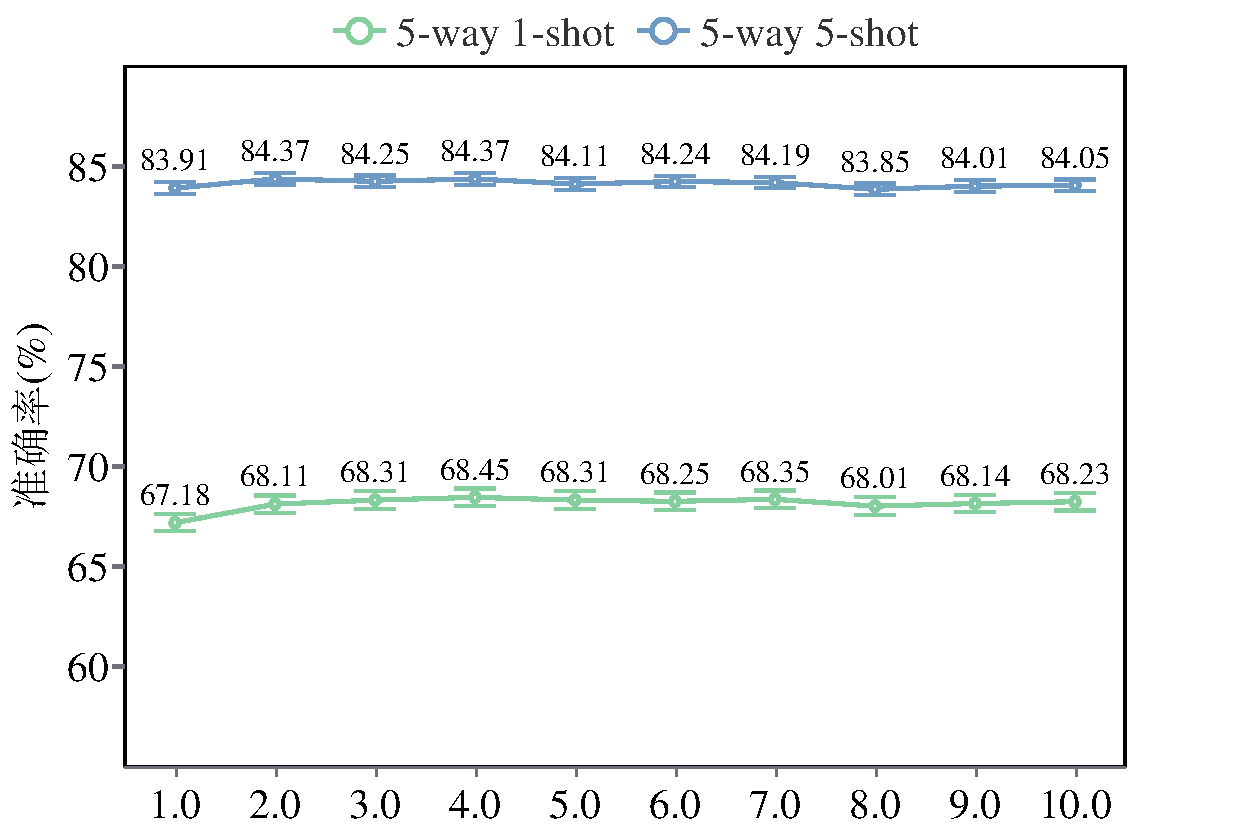
\includegraphics[width=\columnwidth]{figures/MGSRCL/miniImageNet/t1.pdf}
\caption{$\tau_1$}
\label{figure3: t1(mini)}
\end{subfigure}
\begin{subfigure}{0.495\columnwidth}
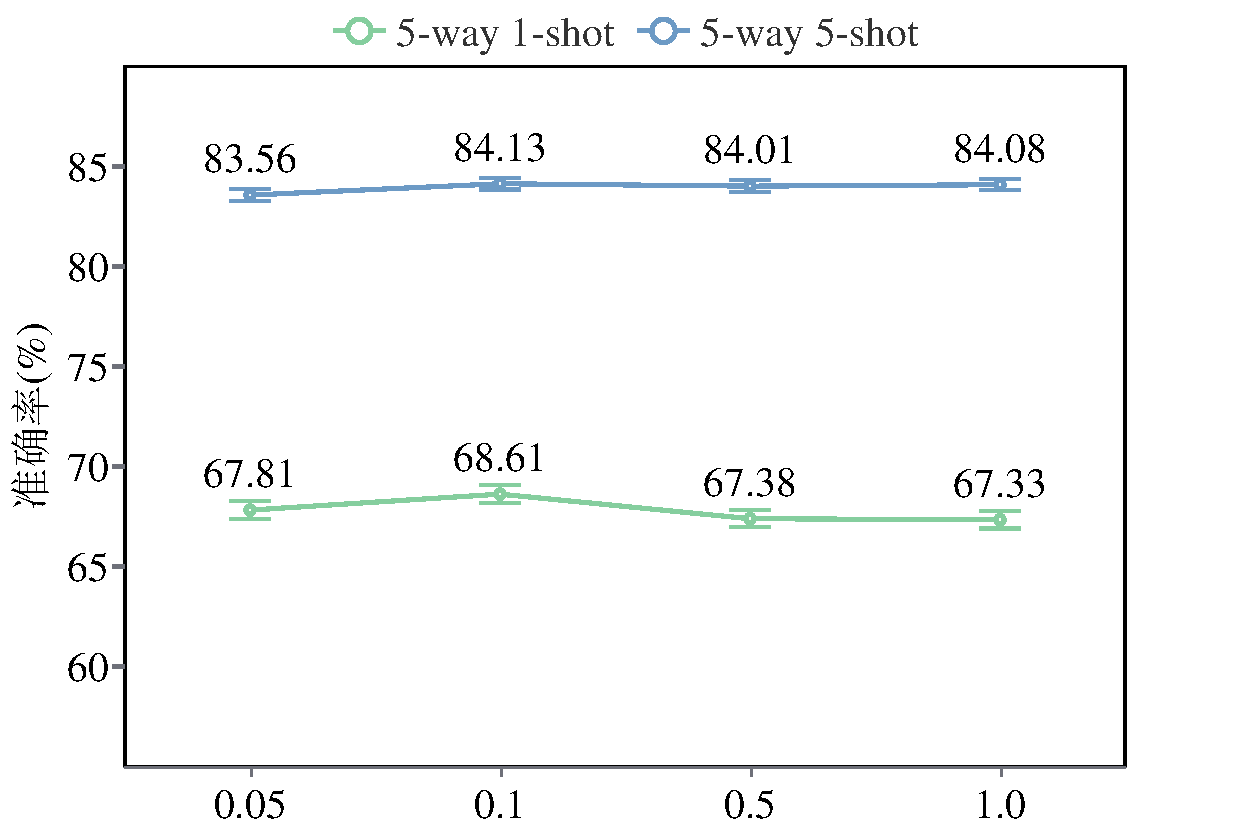
\includegraphics[width=\columnwidth]{figures/MGSRCL/miniImageNet/t2.pdf}
\caption{$\tau_2$}
\label{figure3: t2(mini)}
\end{subfigure}
\bicaption[MGSRCL在miniImageNet数据集上的超参数$\tau_1$和$\tau_2$消融实验]{MGSRCL在miniImageNet数据集上的超参数$\tau_1$和$\tau_2$消融实验。}[Hyperparameters $\tau_1$ and $\tau_2$ ablation experiments of MGSRCL on miniImageNet]{Hyperparameters $\tau_1$ and $\tau_2$ ablation experiments of MGSRCL on miniImageNet.}
\label{figure3: t1 and t2 (mini)}
% \vspace{-10pt}
\end{figure}

\begin{figure}[h!]
\centering
\captionsetup{font={small, stretch=1.312}}
\begin{subfigure}{0.495\columnwidth}
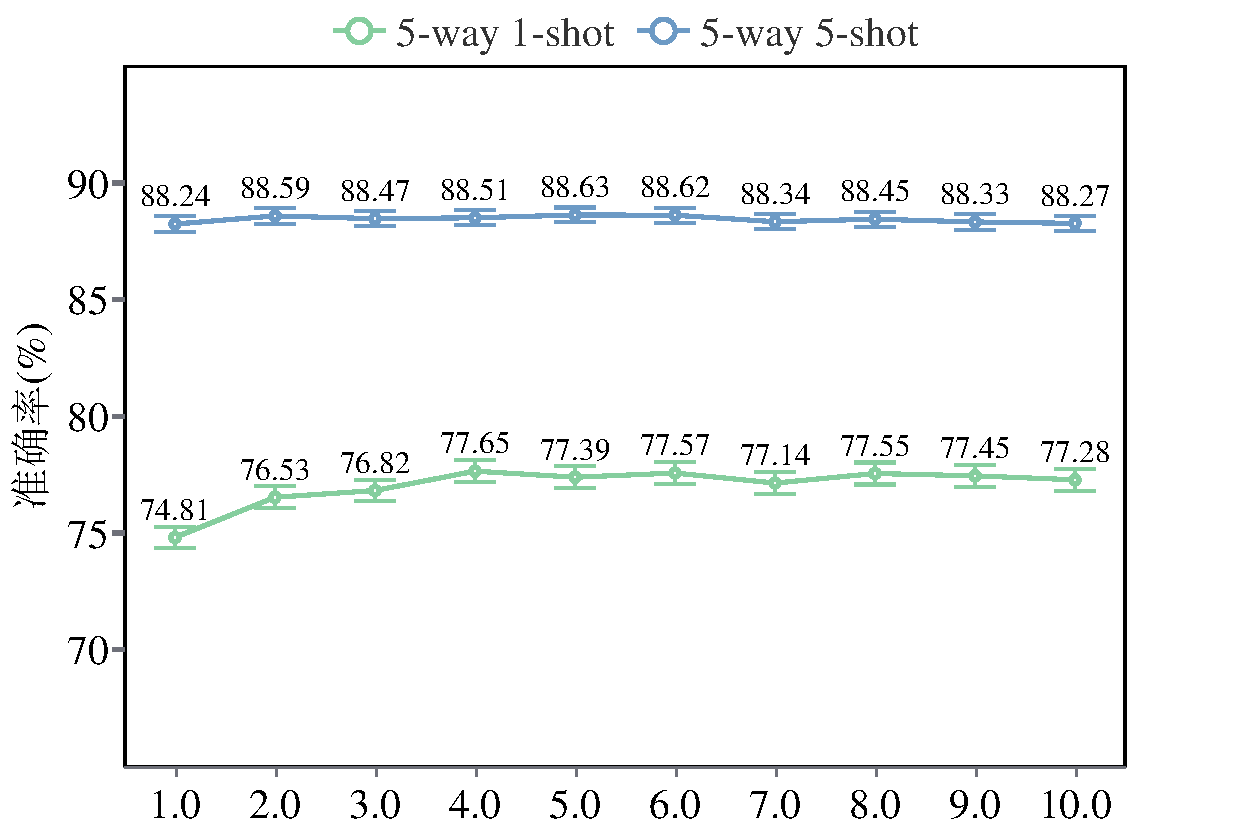
\includegraphics[width=\columnwidth]{figures/MGSRCL/CIFAR-FS/t1.pdf}
\caption{$\tau_1$}
\label{figure3: t1(CIFAR-FS)}
\end{subfigure}
\begin{subfigure}{0.495\columnwidth}
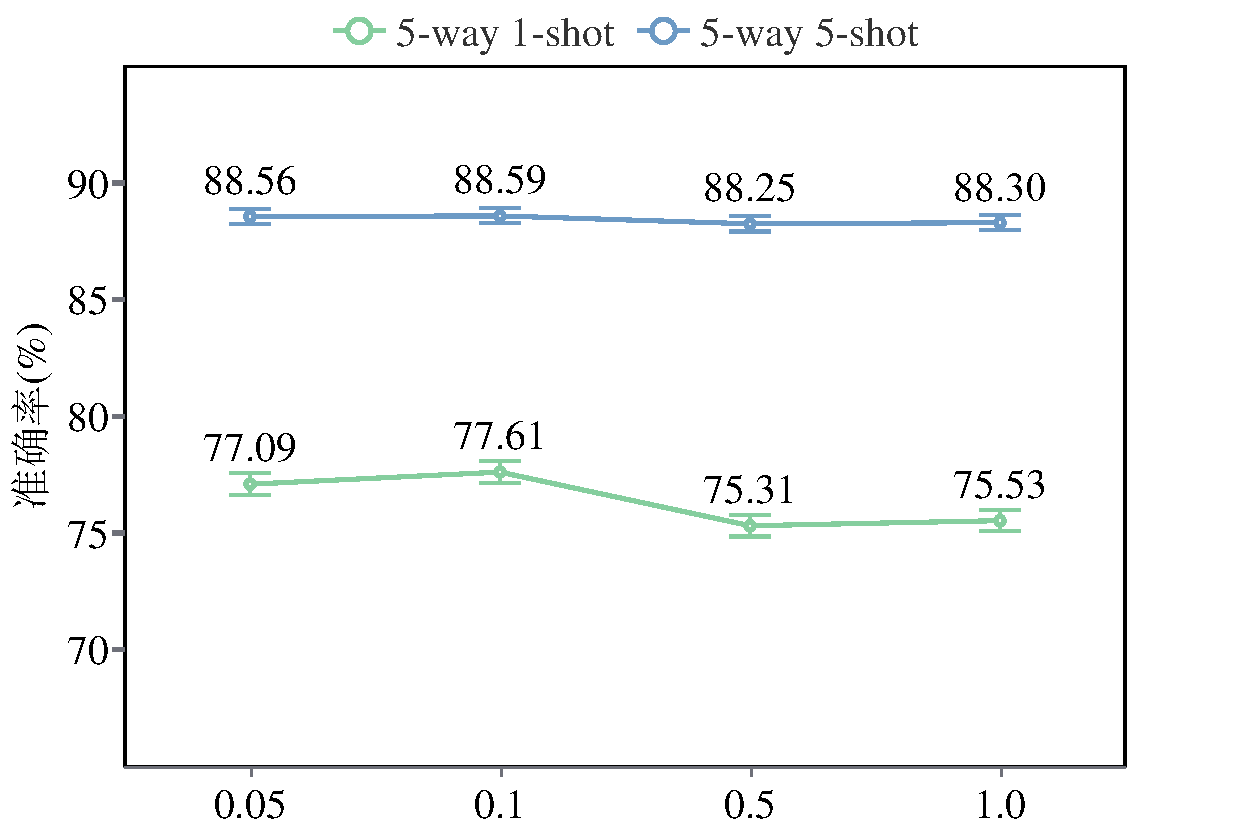
\includegraphics[width=\columnwidth]{figures/MGSRCL/CIFAR-FS/t2.pdf}
\caption{$\tau_2$}
\label{figure3: t2(CIFAR-FS)}
\end{subfigure}
\bicaption[MGSRCL在CIFAR-FS数据集上的超参数$\tau_1$和$\tau_2$消融实验]{MGSRCL在CIFAR-FS数据集上的超参数$\tau_1$和$\tau_2$消融实验。}[Hyperparameters $\tau_1$ and $\tau_2$ ablation experiments of MGSRCL on CIFAR-FS]{Hyperparameters $\tau_1$ and $\tau_2$ ablation experiments of MGSRCL on CIFAR-FS.}
\label{figure3: t1 and t2 (CIFAR-FS)}
% \vspace{-7pt}
\end{figure}

\begin{figure}[h!]
\centering
\captionsetup{font={small, stretch=1.312}}
\begin{subfigure}{0.495\columnwidth}
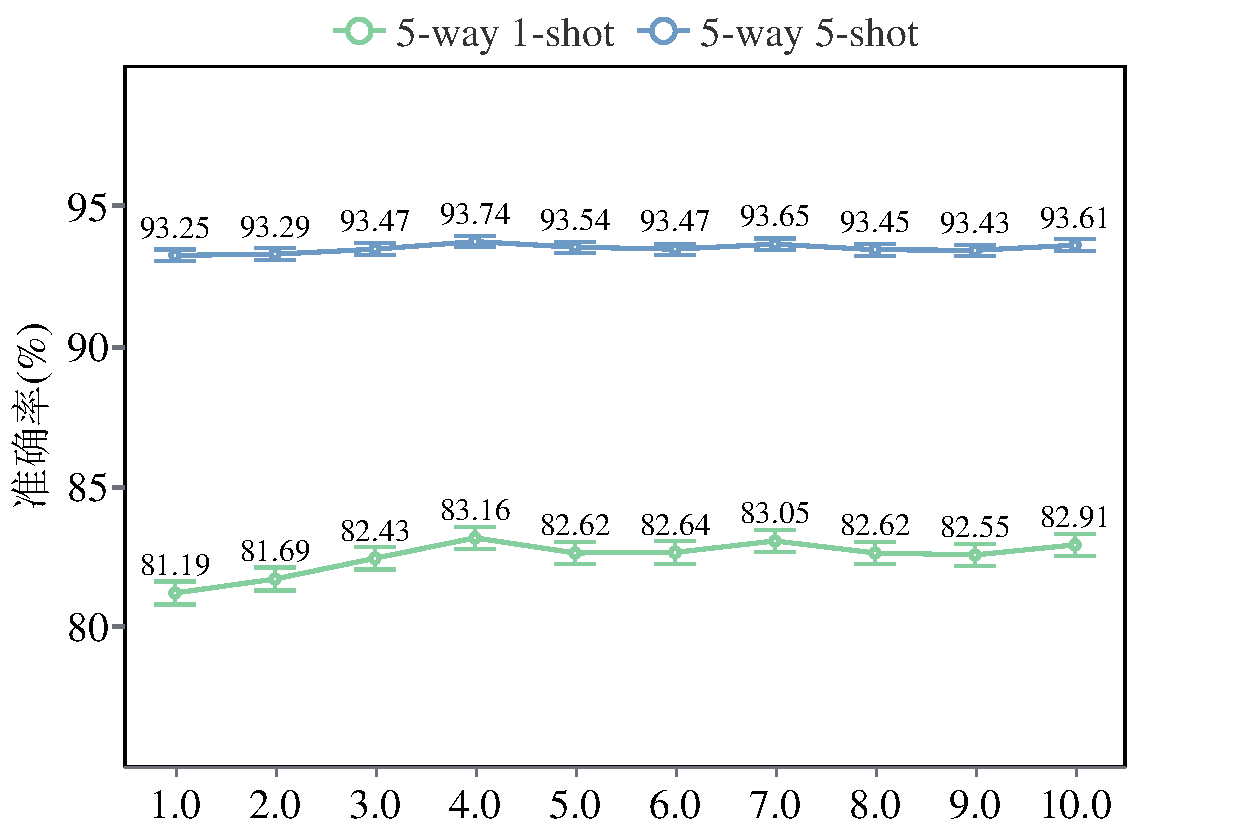
\includegraphics[width=\columnwidth]{figures/MGSRCL/CUB/t1.pdf}
\caption{$\tau_1$}
\label{figure3: t1(CUB)}
\end{subfigure}
\begin{subfigure}{0.495\columnwidth}
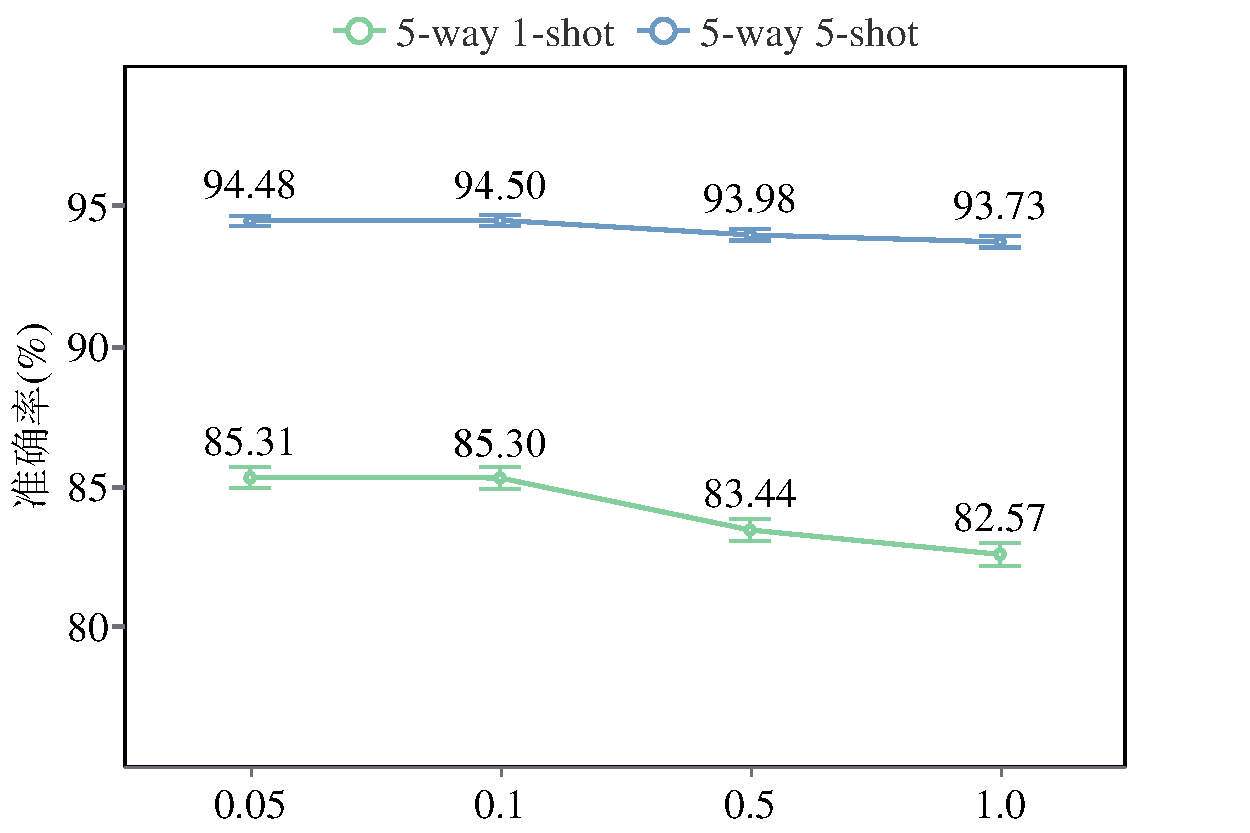
\includegraphics[width=\columnwidth]{figures/MGSRCL/CUB/t2.pdf}
\caption{$\tau_2$}
\label{figure3: t2(CUB)}
\end{subfigure}
\bicaption[MGSRCL在CUB数据集上的超参数$\tau_1$和$\tau_2$消融实验]{MGSRCL在CUB数据集上的超参数$\tau_1$和$\tau_2$消融实验。}[Hyperparameters $\tau_1$ and $\tau_2$ ablation experiments of MGSRCL on CUB]{Hyperparameters $\tau_1$ and $\tau_2$ ablation experiments of MGSRCL on CUB.}
\label{figure3: t1 and t2 (CUB)}
% \vspace{-7pt}
\end{figure}

\textbf{(3)讨论超参数$\tau_1$和$\tau_2$对模型性能的影响}

此外,本文还讨论了温度参数$\tau_1$和$\tau_2$对实验结果的影响。为了更清晰地观察温度参数在对应模块中起到的作用,在讨论温度参数时,本文只保留了相关模块,去除了其他模块。首先,$\tau_1$用于平滑预测输出以提供更多概率分布差异信息,本文令其从1.0到10.0变化,在miniImageNet、CIFAR-FS和CUB三个数据集上评估模型分类性能。如图\ref{figure3: t1 and t2 (mini)}、\ref{figure3: t1 and t2 (CIFAR-FS)}和\ref{figure3: t1 and t2 (CUB)}所示,当$\tau_1$从1.0变化到10.0时,实验结果并未发生显著变化。当执行5-way 1-shot分类任务时,三个数据集都在$\tau_1$设置为4.0时取得了最优结果,执行5-way 5-shot分类任务时,miniImageNet和CUB数据集的也都在$\tau_1$设置为4.0时取得了最优结果,CIFAR-FS则是在$\tau_1$设置为5.0时取得了最优结果。综合考虑,最终将$\tau_1$设置为4.0。$\tau_2$是CCL组件中使用的温度参数。本文评估了当$\tau_2$设置为0.05、0.1、0.5和1.0时的模型性能。除了在CUB数据集的5-way 1-shot分类任务上将$\tau_2$设置为0.05时取得了最优结果,其余数据集以及5-way 5-shot任务均是当$\tau_2 = 0.1$时模型达到了最优结果。因此,在最终模型中,MGSRCL将$\tau_2$设置为0.1。


\begin{figure}[h!]
  \centering
  \captionsetup{font={small, stretch=1.312}}
  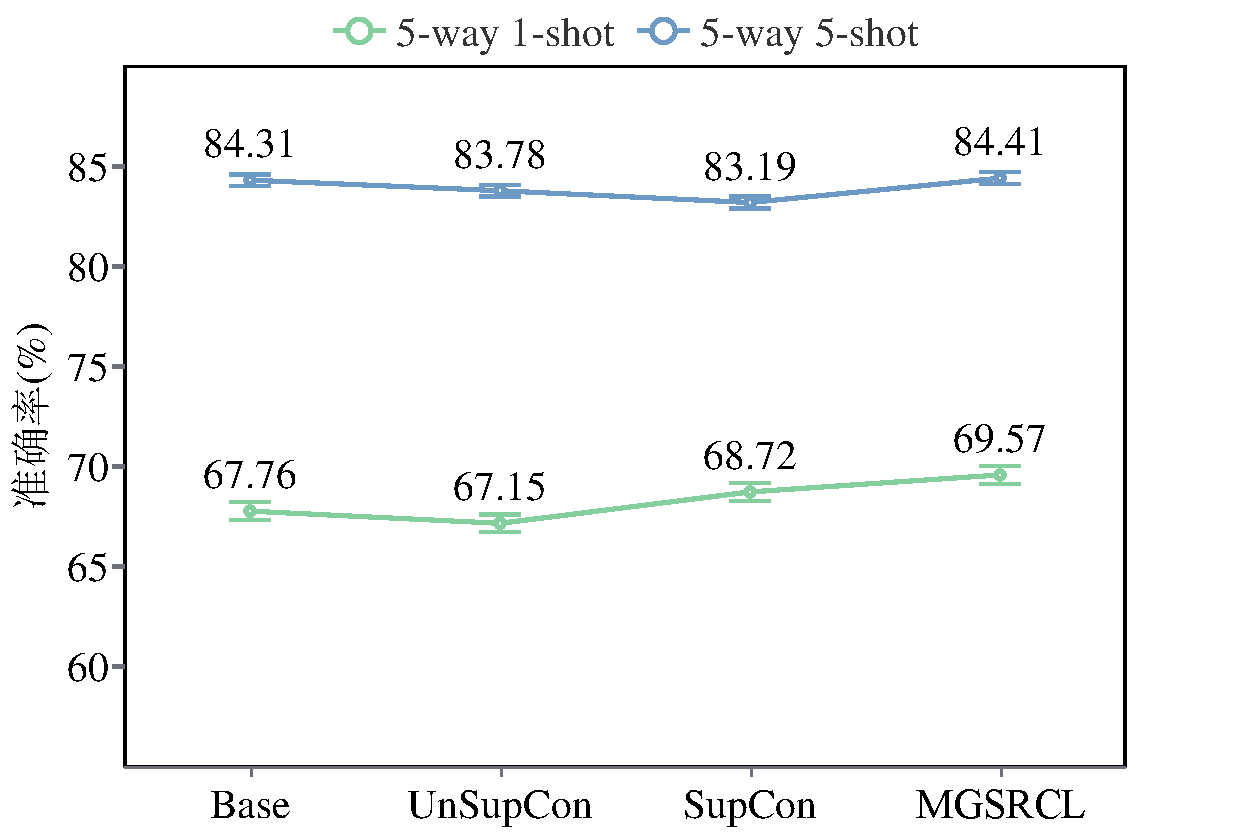
\includegraphics[width=0.6\columnwidth]{figures/MGSRCL/miniImageNet/comparison.pdf}
  \bicaption[在miniImageNet数据集上的不同样本关系挖掘策略对比实验]{在miniImageNet数据集上的不同样本关系挖掘策略对比实验。}[Experimental comparison of different sample relationship mining strategies on miniImageNet]{Experimental comparison of different sample relationship mining strategies on miniImageNet.}
  \label{figure3: comparison(miniImageNet)}
\end{figure}

\begin{figure}[h!]
  \centering
  \captionsetup{font={small, stretch=1.312}}
  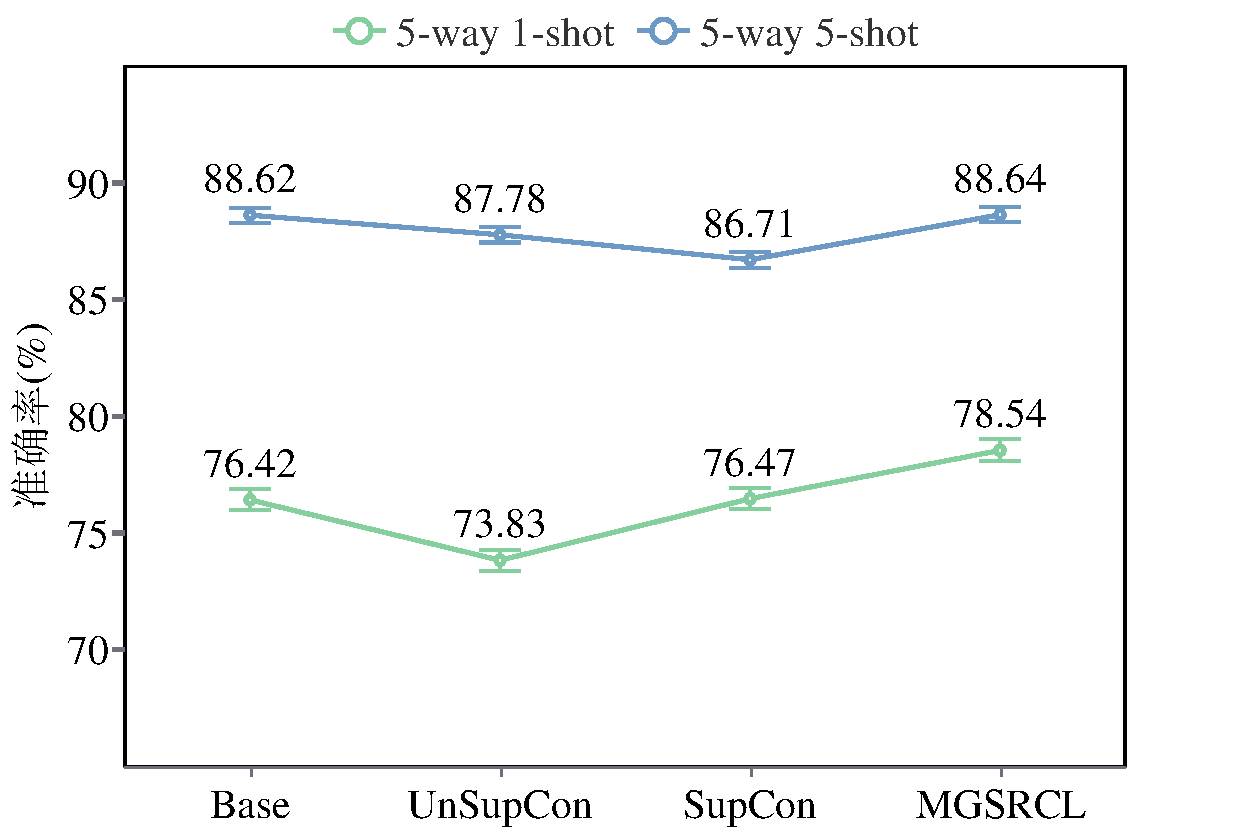
\includegraphics[width=0.6\columnwidth]{figures/MGSRCL/CIFAR-FS/comparison.pdf}
  \bicaption[在CIFAR-FS数据集上的不同样本关系挖掘策略对比实验]{在CIFAR-FS数据集上的不同样本关系挖掘策略对比实验。}[Experimental comparison of different sample relationship mining strategies on CIFAR-FS]{Experimental comparison of different sample relationship mining strategies on CIFAR-FS.}
  \label{figure3: comparison(CIFAR-FS)}
\end{figure}

\begin{figure}[h!]
  \centering
  \captionsetup{font={small, stretch=1.312}}
  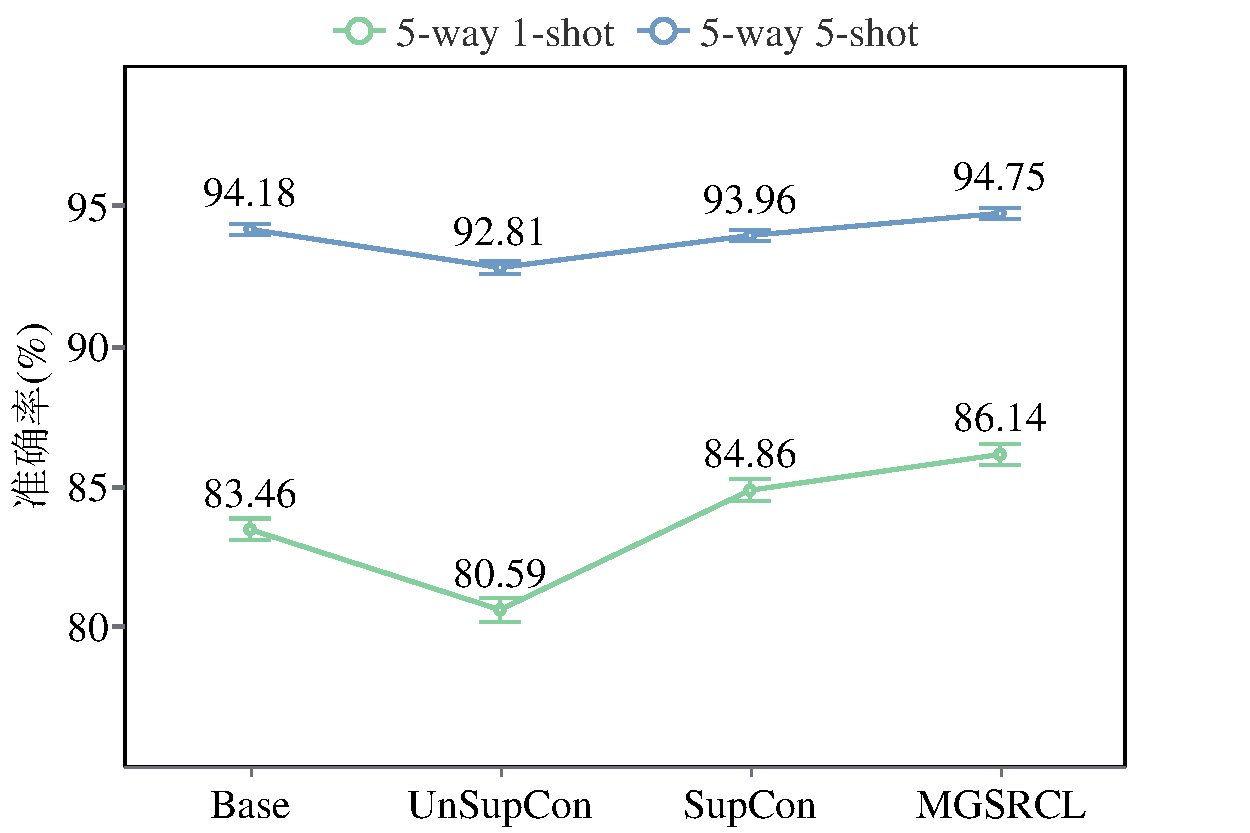
\includegraphics[width=0.6\columnwidth]{figures/MGSRCL/CUB/comparison.pdf}
  \bicaption[在CUB数据集上的不同样本关系挖掘策略对比实验]{在CUB数据集上的不同样本关系挖掘策略对比实验。}[Experimental comparison of different sample relationship mining strategies on CUB]{Experimental comparison of different sample relationship mining strategies on CUB.}
  \label{figure3: comparison(CUB)}
\end{figure}

\textbf{(4)样本关系挖掘策略探讨}

近年来,一些少样本分类方法利用对比学习来挖掘样本关系。然而,这些方法通常直接使用无监督对比学习(Unsupervised Contrastive Learning,简称UnSupCon)\cite{SimCLR}或有监督对比学习(Supervised Contrastive Learning,简称SupCon)\cite{SupCon}作为辅助损失,这使得它们未能充分挖掘样本间的关系。为了表明本文方法相较于这些方法的优越性,本文基于所提出的基础特征学习网络进行了实验\footnote{此处,本文使用了SupCon提供的代码来实现无监督对比学习方法(SimCLR)和有监督对比学习方法(SupCon)。源代码可在\href{https://github.com/HobbitLong/SupContrast}{https://github.com/HobbitLong/SupContrast}获取。}。在实施过程中,UnSupCon和SupCon损失作为辅助损失被直接添加到原基础特征学习网络中,与本文方法相同。如图\ref{figure3: comparison(miniImageNet)}、\ref{figure3: comparison(CIFAR-FS)}和\ref{figure3: comparison(CUB)}所示,在miniImageNet、CIFAR-FS和CUB数据集上,添加UnSupCon后模型性能无论是1-shot分类任务还是5-shot分类任务,结果与基础模型相比都有所下降。这可以归因于UnSupCon将图像的变换视为正样本,而将其他图像视为负样本,会导致其在特征空间将同类样本推远,从而造成性能下降。另一方面,将SupCon整合到模型中并未受到此问题的影响,虽然在5-way 5-shot少样本分类任务上结果略微降低,但其在1-shot分类任务上结果都有所提升,且在miniImageNet与CUB数据集上提升明显。然而,SupCon将一个样本的变换及其同类样本视为相同的关系,这是不合适的,因为一个样本的不同变换应具有一致的语义内容,而同类样本的语义内容应仅相似而不是完全一致。相比之下,本文提出的方法充分考虑了不同粒度的样本关系,并对它们进行了细致地建模,从而在三个数据集上都取得了最优结果,这表明了本文方法更充分地挖掘了样本关系并对其进行了有效建模。


\begin{figure}[h!]
    \centering
    \captionsetup{font={small, stretch=1.312}}
    \begin{subfigure}{0.24\columnwidth}
    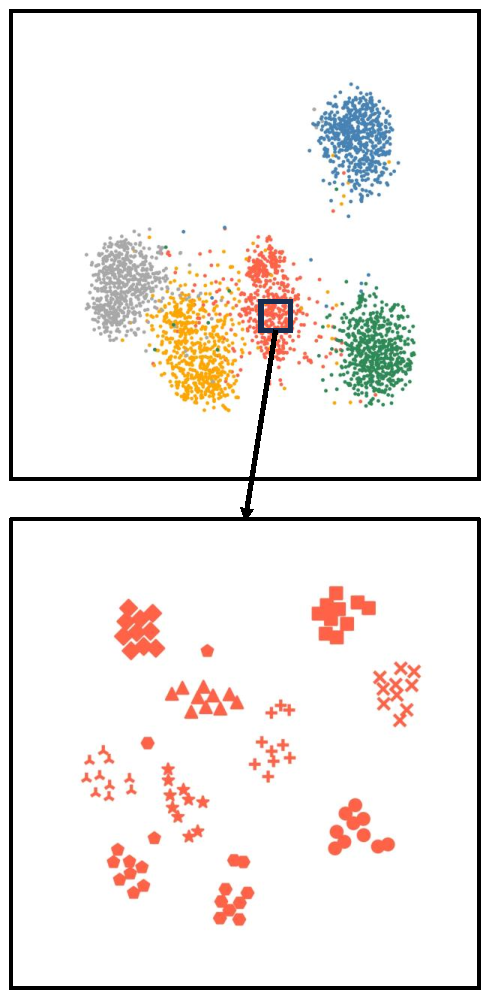
\includegraphics[width=\columnwidth]{figures/MGSRCL/t-SNE/Base.pdf}
    \caption{Base}
    \label{figure3: t-SNE Base}
    \end{subfigure}
    \begin{subfigure}{0.24\columnwidth}
    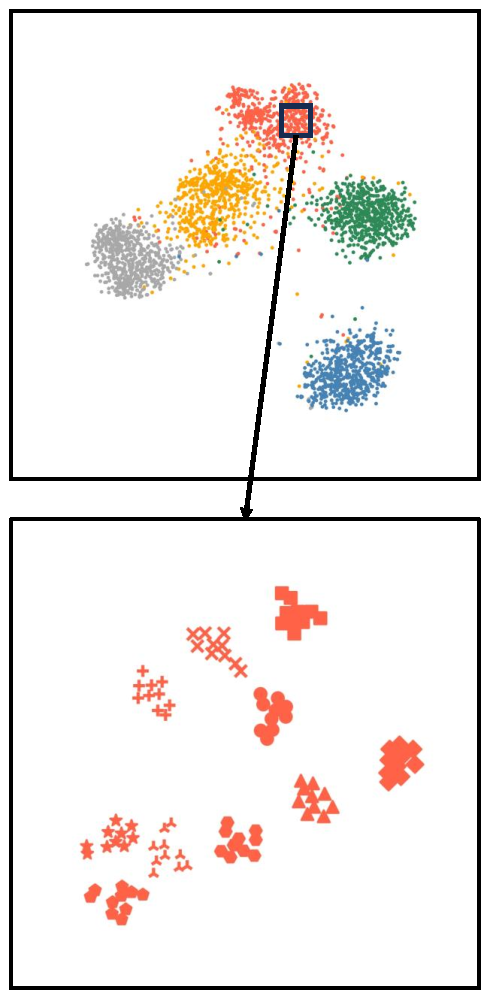
\includegraphics[width=\columnwidth]{figures/MGSRCL/t-SNE/Base + TCL.pdf}
    \caption{Base + TCL}
    \label{figure3: t-SNE Base + TCL}
    \end{subfigure}
    \begin{subfigure}{0.24\columnwidth}
    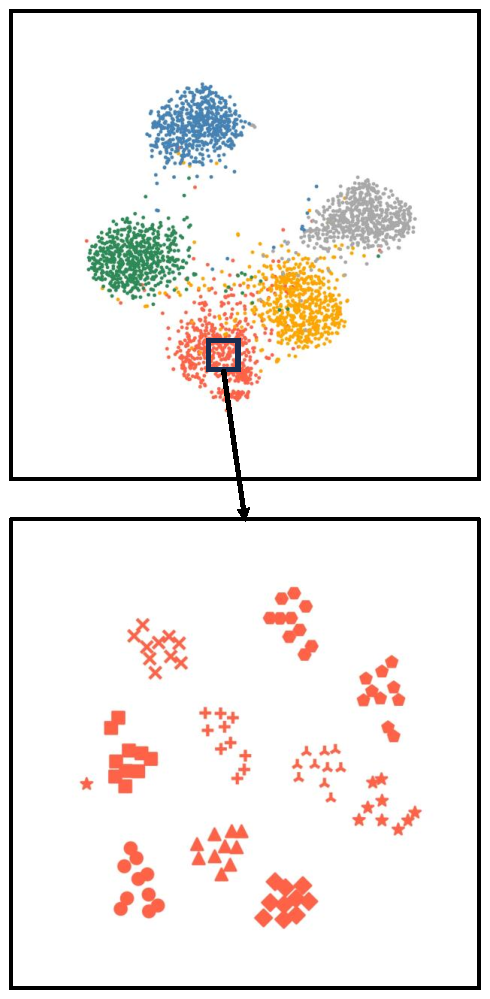
\includegraphics[width=\columnwidth]{figures/MGSRCL/t-SNE/Base + CCL.pdf}
    \caption{Base + CCL}
    \label{figure3: t-SNE Base + CCL}
    \end{subfigure}
    \begin{subfigure}{0.24\columnwidth}
    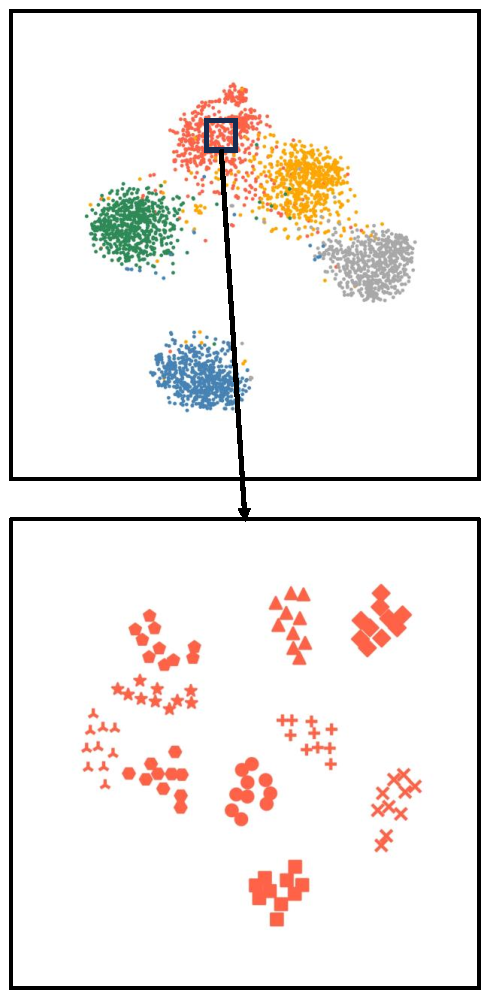
\includegraphics[width=\columnwidth]{figures/MGSRCL/t-SNE/Ours.pdf}
    \caption{MGSRCL}
    \label{figure3: t-SNE MGSRCL}
    \end{subfigure}
    \bicaption[miniImageNet数据集上不同模型所提取特征的t-SNE可视化结果]{miniImageNet数据集上不同模型所提取特征的t-SNE可视化结果。不同颜色代表不同类别(第一行),同一形状代表同一样本的不同变换版本(第二行)。}[The t-SNE visualization results of features extracted by different models on miniImageNet]{The t-SNE visualization results of features extracted by different models on miniImageNet. Different colors represent different categories (first row), and the same shape represents different transformed versions of the same sample (second row).}
    \label{figure3: t-SNE}
\end{figure}


\subsection[\hspace{-2pt}可视化分析]{{\heiti\zihao{4} \hspace{-8pt}可视化分析}}\label{section3: 可视化分析}

为了更好地展示MGSRCL模型的有效性,本文在miniImageNet上随机选取了5个新类,并使用t-SNE对不同模型提取的特征进行了可视化实验,如图\ref{figure3: t-SNE}所示,其中Base表示本文的基础特征学习网络,Base + TCL和Base + CCL分别代表基础特征学习网络整合了TCL模块以及CCL模块,而MGSRCL则代表本文的最终模型。在此图里,第一行展示了类内样本关系和类间样本关系,第二行则是展示了样本内关系,其中第一行图用不同颜色代表不同的类,第二行图则是将同一样本的不同变换版本用同一个形状表示。为便于检验第一行分类边界的质量,本文提供了如下数值数据:$d_1/d_2$,其中$d_1$表示五个类别样本与其样本中心间平均距离的均值(即类内样本内聚度),$d_2$则表征各类别中心之间距离的平均值(即不同类别中心间的离散度)。具体数值如下:(a) Base:1.01,(b) Base + TCL:0.99,(c) Base + CCL:0.91,(d) MGSRCL:0.90。这些数据直观地反映了不同模型在分类边界质量上的表现差异。首先,在第一行图中,可以观察到基础特征学习网络模型Base已经具有明确的分类边界,如图\ref{figure3: t-SNE Base}所示,这证明使用全部基类数据训练一个特征提取网络便可取得一个较好的效果。与Base模型和Base + TCL模型相比,在Base + CCL模型和最终的MGSRCL模型中,同一类别内的样本表现出更好的内聚性,不同类样本之间边界更加明显,这证明了约束同类样本的类内关系和不同类样本的类间关系的有效性。此外,通过约束同一样本在不同变换下的样本内关系,同一样本不同变换版本可以在特征空间保持更好的一致性,如图\ref{figure3: t-SNE Base + TCL}和图\ref{figure3: t-SNE MGSRCL}中的第二行图所示。而在其他模型中,一些变换的特征与其他变换的特征相距甚远,这展示了TCL模块的作用。综上所述,通过可视化实验证明,本文所提方法通过约束多种粒度的样本关系,对不同的样本关系进行了细致有效的建模,使得模型在新类上所提取的特征具有更好的判别性,从而达到了更高的分类准确率。

\section[\hspace{-2pt}本章小结]{{\heiti\zihao{-3} \hspace{-8pt}本章小结}}\label{section3: 本章小结}

本章研究基于多粒度样本关系建模的少样本特征学习算法,针对少样本特征学习模型由于基类数据和新类数据类别不同而面临的模型特征提取能力不足的问题,充分挖掘了多种粒度的样本关系,并通过对比学习对多粒度样本关系进行建模,提出了一种多粒度样本关系对比学习(Multi-Grained Sample Relation Contrastive Learning,简称MGSRCL)方法,以帮助模型提取到更具判别性的样本特征。MGSRCL方法使用一致性学习(TCL)模块通过标签分布对齐约束同一样本的不同变换具有一致的语义内容从而对样本内关系进行建模,以及类对比学习(CCL)模块通过拉近同类样本特征,同时推远不同类样本特征从而对类内样本关系以及类间样本关系进行建模。此外,还利用自监督学习技术令网络学习图像进行了何种变换,来增强基础特征学习网络的特征学习能力。在miniImageNet、tieredImageNet、CIFAR-FS和CUB-200-2011数据集的大量实验表明,MGSRCL在各个少样本基准数据集都取得了优异的性能表现,并且还可以作为预训练模型整合到其他两阶段少样本分类方法中提升它们的分类性能。

综上所述,本章提出的基于多粒度样本关系建模的少样本特征学习算法通过对多种样本关系进行建模,充分挖掘了不同样本间的关系信息,提高了网络所提取特征的质量,并可以为其他少样本分类算法提供优质的预训练网络和高质量的样本特征。


\chapter[\hspace{0pt}基于语义-视觉多空间关系建模的少样本分类研究]{{\heiti\zihao{3}\hspace{0pt}基于语义-视觉多空间关系建模的少样本分类研究}}\label{chapter4: 基于语义-视觉多空间关系建模的少样本分类研究}
\removelofgap
\removelotgap

上一章研究了基于多粒度样本关系建模的少样本特征学习算法,通过充分挖掘不同粒度的样本关系提高了网络所提取特征的质量。然而,该算法仅在视觉空间对多种样本关系进行了建模,忽略了数据集中所隐含的丰富语义信息,限制了模型通过基类数据进行训练来学习新类数据知识的能力。因此,在上一章的基础上,本章主要研究基于语义-视觉多空间关系建模的少样本特征适配算法,通过引入语义信息并与视觉信息进行建模从而丰富模型所获得的信息,增强模型的泛化能力。本章内容共分为四节,\hyperref[section4: 引言]{第一节}介绍研究动机和方法概述;\hyperref[section4: 基于语义-视觉多空间关系建模的少样本特征适配算法]{第二节}介绍本章提出的基于语义-视觉多空间关系建模的少样本特征适配算法;\hyperref[section4: 实验设置及结果分析]{第三节}给出实验设置和结果分析;\hyperref[section4: 本章小结]{第四节}对本章进行小结。

\section[\hspace{-2pt}引言]{{\heiti\zihao{-3} \hspace{-8pt}引言}}\label{section4: 引言}

\subsection[\hspace{-2pt}研究动机]{{\heiti\zihao{4} \hspace{-8pt}研究动机}}\label{section4: 研究动机}

基于视觉的少样本算法,包括基于元学习、度量、数据增强、以及特征学习的方法已经取得了显著进展。然而,这些方法仍面临一些局限性,影响了模型性能的提升。特别是,这些方法往往仅关注样本的视觉信息,忽视了语义信息的潜在价值,使得模型难以从少量样本中学习到具有足够泛化能力的特征表示,这一点直接制约了模型对新类别的识别能力,限制了模型的性能上限。

\begin{figure}[h!]
  \centering
  \captionsetup{font={small, stretch=1.312}}
  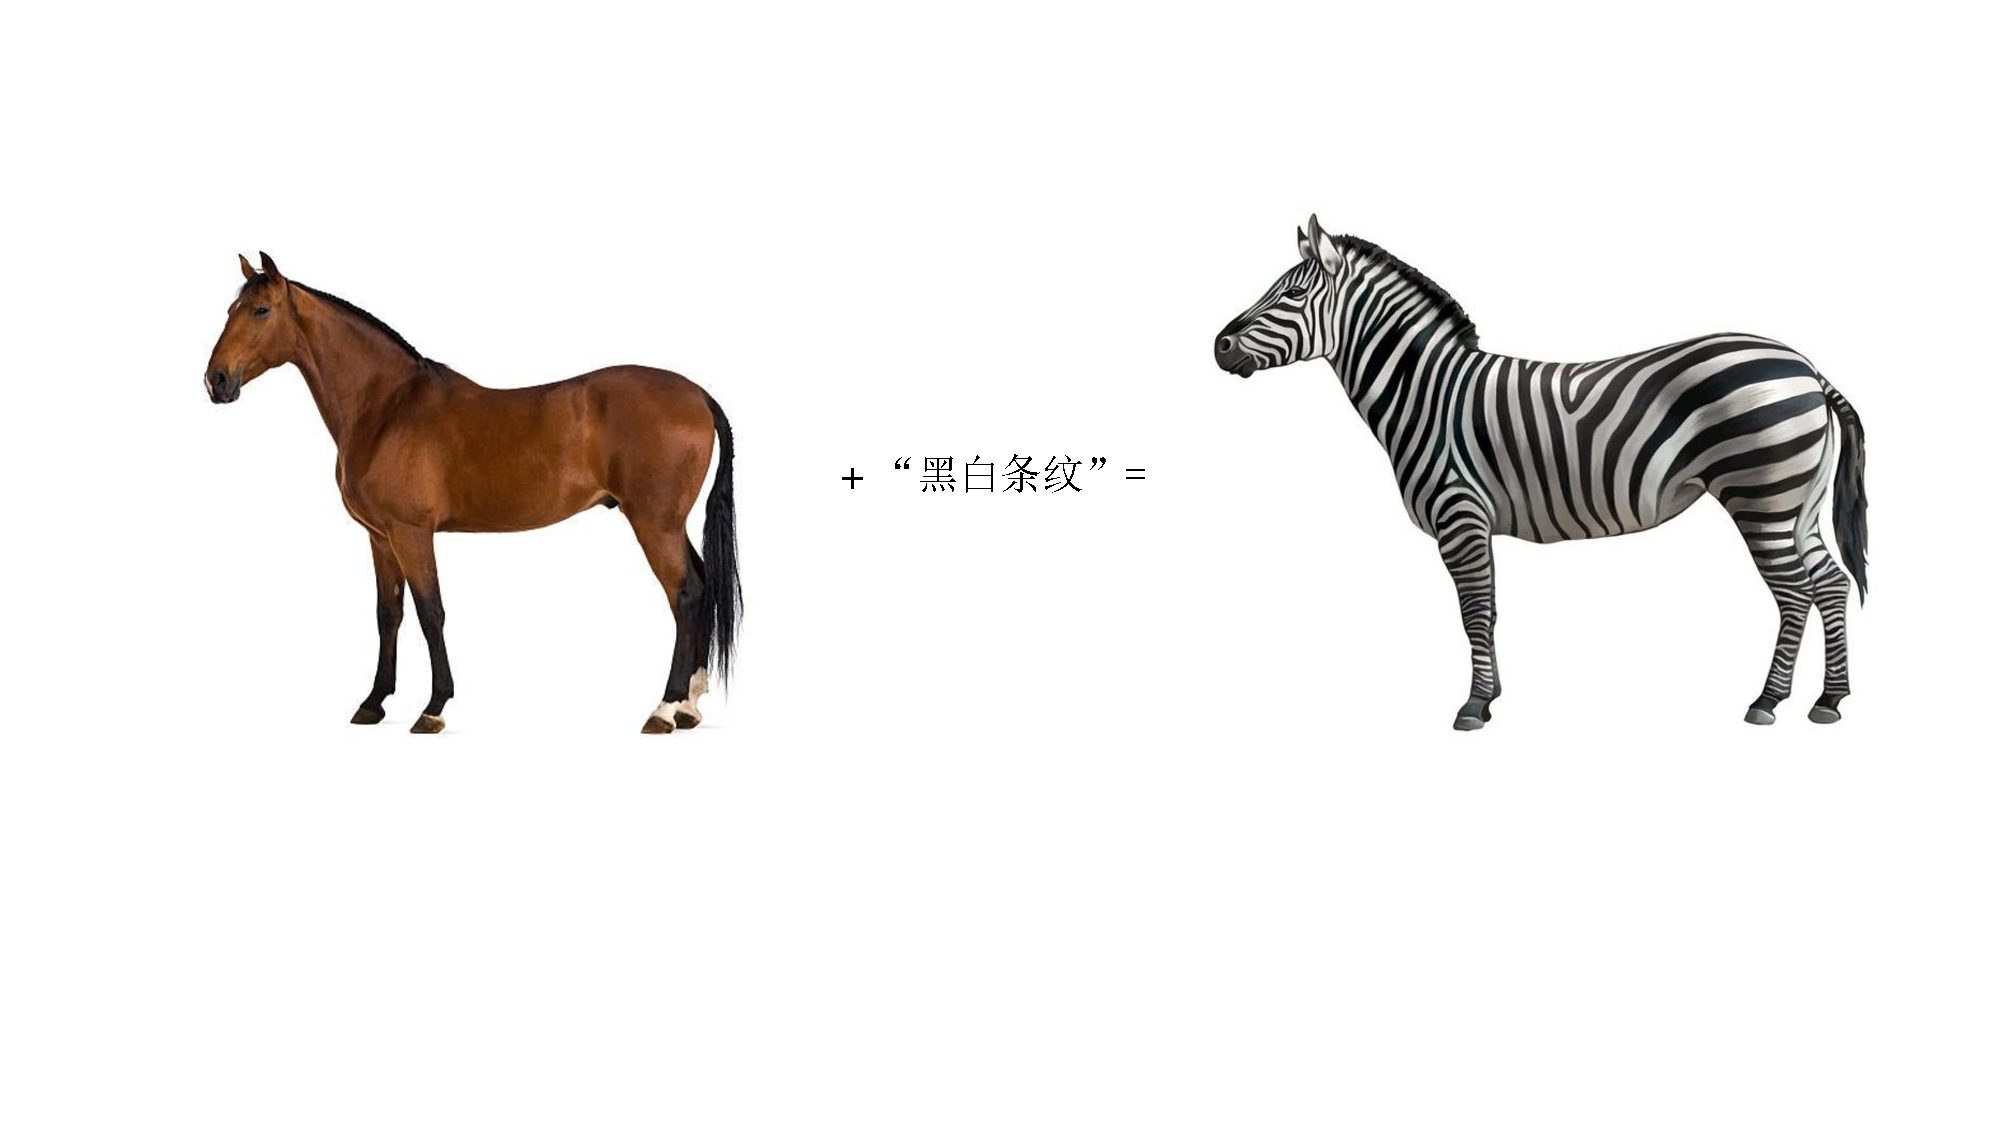
\includegraphics[width=0.9\columnwidth]{figures/SVMSMA/人类认识新类别示意图.pdf}
  \bicaption[人类认识新类别的过程示意]{人类认识新类别的过程示意。以斑马为例进行说明。}[Human process for recognizing new categories]{Human process for recognizing new categories. Illustrated by the example of a zebra.}
  \label{figure4: 人类认识新类别示意图}
\end{figure}

与深度学习模型不同,人类在认识新类别时,依赖的不仅是视觉形象,更多的是对于该形象背后语义的理解和推理。例如,告知某人“斑马”是一种有黑白条纹的“马”,即使在没有看到斑马的情况下,该人也能凭借对“马”的认知和对“黑白条纹”的描述,快速理解并识别“斑马”,如图\ref{figure4: 人类认识新类别示意图}所示。这种通过语义信息桥接的学习过程,是人类认识新事物的一大优势,也是机器学习中尚待深入挖掘的宝贵资源。受到人类认识新物体的启发,研究者认为语义信息在计算机视觉任务中也可发挥同样的作用,尤其是在零样本分类\cite{metric1, metric2, generative1, generative2, 冯耀功2020基于知识的零样本视觉识别综述, 零样本学习, 赵鹏2021一种基于融合重构的子空间学习的零样本图像分类方法}以及少样本分类\cite{KTN, AM3, TRAML, yan2021aligning, CMGNN-DPGN, STVAE, SP-CLIP, 赵凯琳2020小样本学习研究综述, 刘颖2021基于小样本学习的图像分类技术综述, 小样本困境下的深度学习图像识别综述}任务中。为了模拟人类认识新类别的过程从而更好地建立新类与基类之间的联系,很多研究者开始使用自然语言模型\cite{Word2Vec, GloVe, Bert}或多模态模型\cite{Clip}的文本编码器提取类别名称的语义特征作为语义信息,并将其用到少样本分类方法中,如\ref{section1: 研究现状}中所述。


然而,这些工作虽在少样本分类任务中引入了语义信息并进行有效利用,但仍存在一些不足。部分基于特征生成的方法,如STVAE\cite{STVAE}使用语义信息作为条件训练一个特征生成模型。在训练好特征生成模型后,为了提高少样本测试任务中的样本多样性,需要向支持集中添加大量样本,这一做法使得后续的分类器训练时间急剧增长。并且部分生成模型训练过程较为复杂,例如生成对抗网络(Generative Adversarial Networks,简称GAN)\cite{GAN}在训练时需要交替训练生成器和判别器;以及扩散模型(Diffusion Model)\cite{diffusion}在训练时则是需要逐步加噪和去噪过程。基于语义修正的方法\cite{AM3, SP-CLIP}虽然不需要在进行少样本测试任务时对支持集样本进行扩充,但这些方法往往需要设计精细且复杂的信息融合模块,并且这些模块的设计还可能会对自然语言模型或多模态模型所提取的语义信息产生不利影响。具体来说,自然语言模型或多模态模型在大规模语料库上进行了训练,因此提取的语义特征具有较强的泛化性,而过于复杂的信息融合模块可能使得模型在基类数据集产生过拟合问题,削弱这种泛化性,进而降低模型的整体表现。


\subsection[\hspace{-2pt}方法概述]{{\heiti\zihao{4} \hspace{-8pt}方法概述}}\label{section4: 方法概述}

为解决上述问题并充分利用语义信息以补充视觉信息,进而提升少样本分类任务的准确率,本章提出了一种基于语义-视觉多空间关系建模的少样本特征适配算法,即语义-视觉多空间映射适配(Semantic-Visual Multi-Space Mapping Adapter,简称SVMSMA)模型。SVMSMA模型以一种简单的特征适配方式利用语义信息,不需要对语义特征进行复杂信息融合操作,从而避免了降低语义特征泛化性的问题,并能够有效丰富样本特征的信息来源,弥补仅使用视觉信息的不足。

由于在少样本分类测试任务中,查询集只能够获得视觉信息(已知语义信息则已知类别),为了执行测试任务以及使用跨模态分类任务(将在后续介绍)对网络进行优化,本文采用将语义信息映射到视觉空间的方案对两种信息之间的关系进行建模。因此,本文首先提出了一个语义-视觉多空间映射网络(Semantic-Visual Multi-Space Mapping Network,简称SVMSMN),采用两种可独立使用的模式将语义信息映射到视觉空间:1)单模态映射,2)多模态映射。单模态映射是指使用类似零样本学习的思想,仅将语义信息映射到视觉空间,在执行测试任务时仅使用语义信息来获取语义映射特征,并不会使用到支持集样本的视觉特征。多模态映射则是在语义信息的基础上使用视觉信息对其进行补充,将两个模态信息融合后再映射到视觉空间,以对支持集样本的视觉信息加以利用。

另外,为了建模语义信息与视觉信息的关系,从而能够使用语义映射特征对支持集的视觉特征进行补充,提升少样本分类任务性能,本文提出了两个模块以对语义-视觉多空间映射网络进行优化使得语义映射特征适配视觉空间,分别是1)跨模态分类(Cross-Modal Classification,简称CMC)模块,2)跨模态特征对齐(Cross-Modal Feature Alignment,简称CMFA)模块。其中,跨模态分类模块使用预训练的视觉特征提取网络的分类器对上述语义映射特征进行分类,以对映射网络进行优化使得每个类别的语义信息和对应的视觉特征建立联系。跨模态特征对齐模块则是将语义映射特征与通过视觉特征提取网络得到的视觉特征原型进行对齐,以这种方式对映射后的特征进行修正,使其更接近类别原型,从而能够取得更好的分类结果。

本章方法同样在四个少样本分类数据集进行了实验,包括miniImageNet\cite{vinyals2016matching}、tieredImageNet\cite{ren2018meta}、CIFAR-FS\cite{bertinetto2019meta},以及CUB-200-2011\cite{wah2011caltech}。实验结果表明,本章方法可有效建模语义-视觉空间关系,利用语义信息对视觉信息进行补充,从而取得优异的少样本分类结果。

\section[\hspace{-2pt}基于语义-视觉多空间关系建模的少样本特征适配算法]{{\heiti\zihao{-3} \hspace{-8pt}基于语义-视觉多空间关系建模的少样本特征适配算法}}\label{section4: 基于语义-视觉多空间关系建模的少样本特征适配算法}

在本节中,首先对使用语义信息的少样本分类任务及其符号定义进行介绍;然后对所提出的基于语义-视觉多空间关系建模的特征适配模型进行简要介绍;接下来详细介绍了所提模型的各个模块及其损失优化;最后介绍了模型总体优化目标以及模型推理过程。

\subsection[\hspace{-2pt}符号定义]{{\heiti\zihao{4} \hspace{-8pt}符号定义}}\label{section4: 符号定义}

在本章中,由于引入了语义信息,各种符号定义与第三章有所不同。基类数据集与新类数据集分别表示为:
\begin{equation}
\begin{aligned}
  &\mathcal{D}_{base} = \{(x, y, s)|x \in X^{base}, y \in Y^{base}, s \in S^{base}\},\\
  &\mathcal{D}_{novel} = \{(x, y, s)|x \in X^{novel}, y \in Y^{novel}, s \in S^{novel}\}.
\end{aligned}
\end{equation}
其中,$\mathcal{D}_{base}$所包含的类别$\mathcal{C}_{base}$和$\mathcal{D}_{novel}$所包含的类别$\mathcal{C}_{novel}$不相交。另外,$x$、$y$、$s$分别表示样本图像、样本标签、以及样本语义特征;$X^{base}$、$Y^{base}$、$S^{base}$分别表示基类样本图像集合、标签集合、语义特征集合;$X^{novel}$、$Y^{novel}$、$S^{novel}$则分别表示新类样本图像集合、标签集合、语义特征集合。在本章中,语义特征是通过将类别名称/提示文本+类别名称输入自然语言处理模型或者多模态模型的文本编码器得到的。

与上一章相同,本章也通过在$\mathcal{D}_{novel}$中采样大量少样本分类任务并计算平均准确率来评估模型性能。不同的是,本章所采样少样本分类任务的支持集$\mathcal{S}_{\mathcal{T}}$除了包含样本图像$x_i$以及样本标签$y_i$外,还包含了样本语义特征$s_i$。因此,支持集表示为:
\begin{equation}
  \mathcal{S}_{\mathcal{T}} = \{(x_i, y_i, s_i)|x_i \in X^{\mathcal{T}}, y_i \in Y^{\mathcal{T}}, s_i \in S^{\mathcal{T}}\}_{i=1}^{N \times K},
\end{equation}
其中,$X^{\mathcal{T}}$、$Y^{\mathcal{T}}$、$S^{\mathcal{T}}$分别表示所采样任务的样本图像集合、标签集合、语义特征集合;$N$和$K$则是表示类别数目以及每个类别样本数目。查询集的样本类别未知,因此无法获取其语义特征,表示为:
\begin{equation}
  \mathcal{Q}_{\mathcal{T}} = \{(x_i, y_i)|x_i \in X^{\mathcal{T}}, y_i \in Y^{\mathcal{T}}\}_{i=1}^{N \times Q},
\end{equation}
$Q$表示每个类别用作测试的样本数目。

\begin{figure}[h!]
  \centering
  \captionsetup{font={small, stretch=1.312}}
  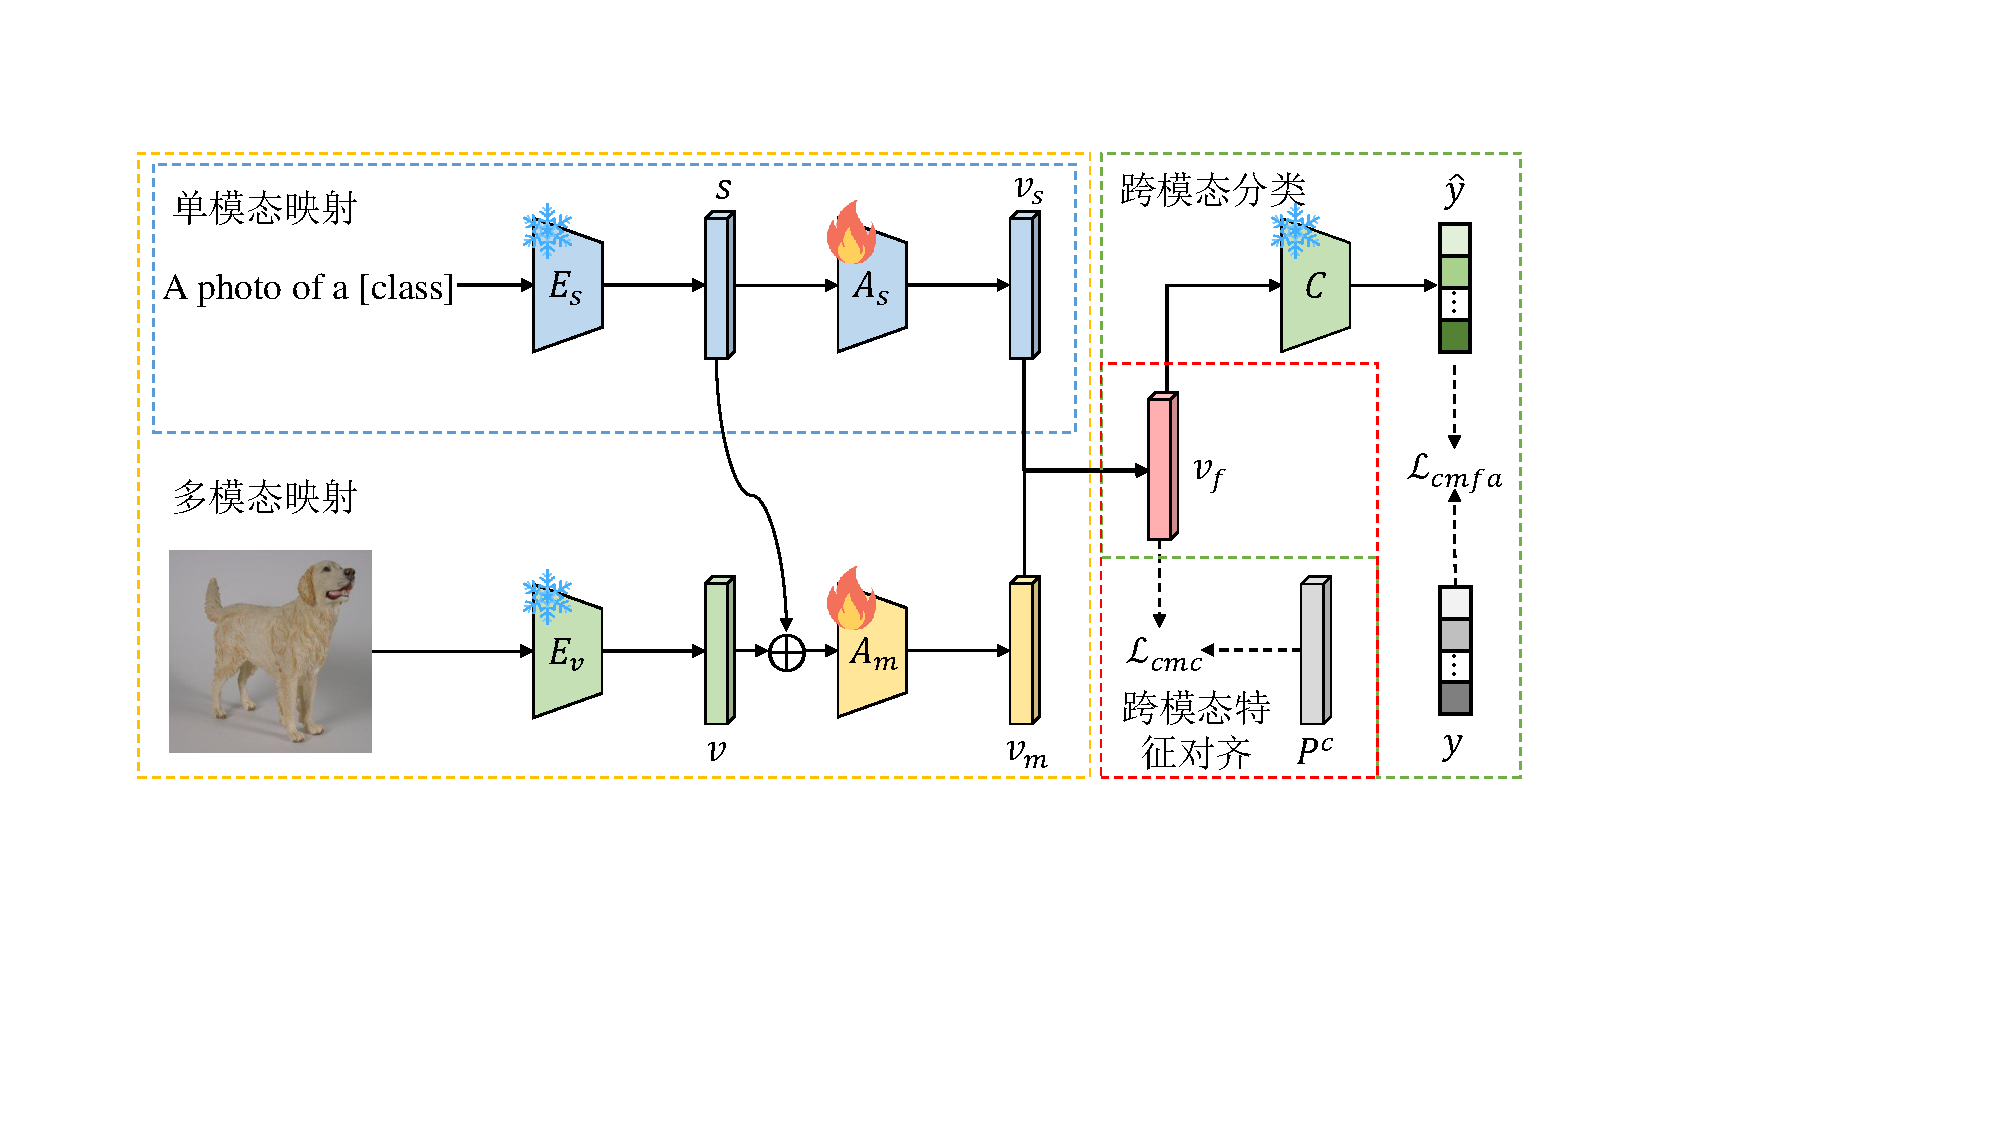
\includegraphics[width=1.0\columnwidth]{figures/SVMSMA/model.pdf}
  % \captionsetup{justification=justified,singlelinecheck=false}
  \bicaption[语义-视觉多空间映射适配模型示意图]{语义-视觉多空间映射适配模型示意图。该模型包含一个视觉特征提取网络$E_v$、一个语义特征提取网络$E_s$,两个语义-视觉多空间映射网络$A_s$与$A_m$,以及一个分类器$C$。在此图中,$v$与$s$分别表示视觉特征与语义特征,$v_s$与$v_m$则是通过$A_s$与$A_m$获得的映射特征,统称为$v_f$。$\widehat{y}$、$y$、$P^c$分别表示预测输出、真实标签和对应类原型特征。$\mathcal{L}_{cmc}$与$\mathcal{L}_{cmfa}$表示跨模态分类损失和跨模态特征对齐损失。另外,模型训练过程中,$E_v$、$E_s$与$C$的参数都被冻结。}[Illustration of Semantic-Visual Multi-Space Mapping Adapter]{Illustration of Semantic-Visual Multi-Space Mapping Adapter. The model includes a visual feature extractor $E_v$, a semantic feature extractor $E_s$, two semantic-visual multi-space mapping networks $A_s$ and $A_m$, and a classifier $C$. In this figure, $v$ and $s$ represent the visual and semantic features, respectively, while $v_s$ and $v_m$ are the mapping features obtained through $A_s$ and $A_m$, collectively referred to as $v_f$. $\widehat{y}$, $y$, and $P^c$ denote the predicted output, true label, and corresponding class prototype features, respectively. $\mathcal{L}_{cmc}$ and $\mathcal{L}_{cmfa}$ represent the cross-modal classification loss and cross-modal feature alignment loss, respectively. Additionally, during the model training process, the parameters of $E_v$, $E_s$, and $C$ are all frozen.}
  \label{figure4: model}
\end{figure}

\subsection[\hspace{-2pt}整体框架]{{\heiti\zihao{4} \hspace{-8pt}整体框架}}\label{section4: 整体框架}

本章提出了一种基于语义-视觉多空间关系建模的少样本特征适配算法,即语义-视觉多空间映射适配模型(Semantic-Visual Multi-Space Mapping Adapter,简称SVMSMA),用以建模样本的语义-视觉多空间关系。该算法旨在利用语义信息作为视觉信息的补充,丰富模型所提取样本特征的信息来源,提升模型在新类上的泛化能力。如图\ref{figure4: model}所示,SVMSMA模型主要包含三个部分:语义-视觉多空间映射网络(Semantic-Visual Multi-Space Mapping Network,简称SVMSMN),跨模态分类(Cross-Modal Classification,简称CMC)模块,以及跨模态特征对齐(Cross-Modal Feature Alignment,简称CMFA)模块。具体来说,语义-视觉多空间映射网络(SVMSMN)用以将语义特征映射到视觉空间,以方便后续与视觉特征进行建模;跨模态分类(CMC)模块通过对映射后的语义特征执行分类任务,以优化映射网络从而使得语义特征与视觉特征建立联系;跨模态特征对齐(CMFA)模块则是将映射后的语义特征与视觉特征原型进行对齐,以对映射后的特征进行修正从而获得更接近类别原型的特征。接下来,本节将会对SVMSMA模型的每个部分进行详细介绍。

\subsection[\hspace{-2pt}语义-视觉多空间映射网络]{{\heiti\zihao{4} \hspace{-8pt}语义-视觉多空间映射网络}}\label{section4: 语义-视觉多空间映射网络}

以方便后续对语义信息与视觉信息进行建模,需要将语义特征和视觉特征投影到相同空间。为了充分利用自然语言处理模型或多模态模型在大规模语料库上对类别名称建立的联系,以及后续建模算法(包括跨模态分类以及跨模态特征对齐)的进行,本文采用将语义特征映射到视觉空间的方式,提出了语义-视觉多空间映射网络(Semantic-Visual Multi-Space Mapping Network,简称SVMSMN),以使得两种信息的特征向量维度一致。本章提出的语义-视觉多空间映射网络可分为两种模式:1)单模态映射,2)多模态映射。这两种模式的核心区别在于它们所处理特征信息的模态种类不同,以下分别对其进行介绍。

\textbf{(1)单模态映射}

单模态映射模式专注于语义信息的处理,其核心思想借鉴了零样本分类领域的思想。该模式的目标是建立一个能够将纯语义信息(例如,文本描述或类别名称)映射至视觉特征空间的高效网络。在实践中,这一过程首先通过语义特征提取网络$E_s$,将类名或提示文本$text$转化为语义特征$s$,
\begin{equation}
  \label{equation4: text to s}
  s = E_s(text).
\end{equation}
随后,单模态映射网络$A_s$负责将这些语义特征映射至视觉空间,生成对应的单模态映射特征$v_s$。该过程可表示为以下公式,
\begin{equation}
  \label{equation4: s to v_s}
  \quad v_s = A_s(s).
\end{equation}

值得注意的是,在本章少样本分类的测试任务中,单模态映射不依赖于任何视觉信息,即不需要支持集的视觉特征参与,这一点使得其更类似于零样本分类的设置。

\textbf{(1)多模态映射}

与单模态映射相比,多模态映射模式采用了一种更为综合和动态的策略,它不仅处理语义信息,同时也将视觉信息作为语义信息的补充。这种模式首先利用预训练的视觉特征提取网络$E_v$,从给定样本图像$x$中提取出丰富的视觉特征$v$,
\begin{equation}
  \label{equation4: x to v}
  v = E_v(x),
\end{equation}
另外通过语义特征提取网络$E_s$获取相应的语义特征$s$,如公式\ref{equation4: text to s}所示。接着,需要对视觉特征和语义特征进行融合,并使用多模态映射网络$A_m$将融合后的多模态特征映射到视觉空间,得到对应的多模态映射特征$v_m$,本章所采用的融合方式为最简单的concat操作。该过程可表达为以下公式,
\begin{equation}
  \label{equation4: v s to v_m}
  v_m = A_m(\text{concat}(v, s)),
\end{equation}

在少样本分类任务中,这种多模态映射模式能够充分利用支持集的视觉特征,以及待分类样本的语义特征,使得所提取特征的信息来源更加丰富,从而更好地适应少样本分类的挑战。

训练过程中,无论是单模态映射模式还是多模态映射模式,SVMSMN都以适配器(Adapter)的方式被插入视觉特征提取网络$E_v$与语义特征提取网络$E_s$之后,视觉特征分类器$C$之前,以在不牺牲特征提取网络泛化能力的前提下,适应本文后续提出的跨模态分类任务和跨模态特征对齐任务。

\subsection[\hspace{-2pt}语义-视觉多空间关系建模算法]{{\heiti\zihao{4} \hspace{-8pt}语义-视觉多空间关系建模算法}}\label{section4: 语义-视觉多空间关系建模算法}

为了建模语义信息和视觉信息的关系,本章提出了两个模块对上一节介绍的语义-视觉多空间映射网络进行优化:1)跨模态分类模块,2)跨模态特征对齐模块。以下将分别对两个模块及其损失进行介绍。

\textbf{(1)跨模态分类}

跨模态分类(Cross-Modal Classification,简称CMC)模块旨在通过分类任务对语义-视觉多空间映射网络进行优化,强化语义信息与视觉信息之间的联系,使得映射后的语义特征能够与实际视觉特征具有一致性。该模块利用预训练视觉特征提取网络时得到的分类器,对通过映射网络得到的单模态或多模态映射特征进行分类,从而促使模型学习到每个类别的语义信息和对应视觉信息之间的紧密对应关系。

具体而言,跨模态分类模块接收映射网络输出的单模态映射特征$v_s$或多模态映射特征$v_m$作为输入,利用分类器$C$计算每个样本的概率分布。该过程可以表达为以下公式,
\begin{equation}
  \label{equation4: softmax}
  \widehat{y} = \text{Softmax}(C(v_f)),
\end{equation}
其中$v_f$表示输入的映射特征,可以为$v_s$或$v_m$,$\widehat{y}$表示样本的预测概率分布。跨模态分类的损失函数采用交叉熵损失,表示为以下公式,
\begin{equation}
  \label{equation4: CMC_loss}
  \mathcal{L}_{cmc} = -\frac{1}{N}\sum_{i=1}^{N}y_i \text{log}\widehat{y}_i,
\end{equation}
其中$N$表示样本数目,$y_i$表示样本类别标签。通过最小化$\mathcal{L}_{cmc}$,模型能够学习到如何将语义信息有效映射到视觉空间,并确保映射后的语义特征与实际类别之间具有高度的一致性。

\textbf{(2)跨模态特征对齐}

跨模态特征对齐(Cross-Modal Feature Alignment,简称CMFA)模块的目的是通过对齐映射特征$v_f$和视觉特征提取网络得到的视觉特征原型$P^c$,以对$v_f$进行修正,使其更接近类别原型,从而提高映射特征$v_f$对每个类别的代表性,进一步提升少样本分类的准确性。

该模块首先计算每个类别的视觉特征原型$P^c$,即该类别所有样本视觉特征的平均值。$P^c$可通过以下公式计算,
\begin{equation}
  \label{equation4: prototype}
  {P}^{c} = \frac{1}{|X^c|} \sum_{i=1}^{|X^c|} v_i,
\end{equation}
其中$X^c$是类别$c$中所有样本的集合,$v_i$是样本$x_i$的视觉特征。接着,CMFA模块计算映射后的视觉特征和对应类别原型之间的距离,并通过最小化该距离来实现特征对齐,该损失函数表示为以下公式,
\begin{equation}
  \label{equation4: CMFA_loss}
  \mathcal{L}_{cmfa} = \frac{1}{N} \sum_{i=1}^{N} || v_{fi} - P^{y_i} ||_2^2,
\end{equation}
其中$|| \cdot ||_2$表示L2范数,用于衡量映射特征$v_{fi}$与对应类别原型$P^{y_i}$之间的欧式距离。通过优化损失函数$\mathcal{L}_{cmfa}$,模型能够引导语义映射特征更贴近于类别的视觉中心,从而获得更具代表性的样本特征,在少样本分类的测试阶段实现更高的准确率。

\subsection[\hspace{-2pt}模型优化]{{\heiti\zihao{4} \hspace{-8pt}模型优化}}\label{section4: 模型优化}

结合公式\ref{equation4: CMC_loss}和\ref{equation4: CMFA_loss},本文提出的SVMSMA模型总体损失函数可以表示为:
\begin{equation}
  \label{equation4: total_loss}
  \mathcal{L}_{total} = \mathcal{L}_{cmc} + \alpha \cdot \mathcal{L}_{cmfa},
\end{equation}
其中,$\alpha$是用来衡量不同损失权重的超参数。

SVMSMA模型在整个基类数据集进行训练,没有采用元学习的方式,并通过最小化损失函数$\mathcal{L}_{total}$对模型参数进行联合优化,通过引入语义信息并对语义-视觉多空间关系进行建模,从而能够丰富模型所获得的信息,更好地迁移在基类数据集上学习到的知识,提升模型的泛化能力。另外,本文中所使用的语义特征提取网络$E_s$基于现有的自然语言处理模型或多模态模型的文本编码器,视觉特征提取网络$E_v$基于使用基类数据集的图像样本预训练的特征提取网络,分类器$C$基于训练视觉特征提取网络时所使用的分类器,$E_s$、$E_v$和$C$的网络参数在本章模型训练时都是冻结的,换句话说,只有单模态映射网络$A_s$和多模态映射网络$A_m$参与了网络参数更新,并且这两个网络是单独进行训练的。

\begin{figure}[h!]
  \centering
  \captionsetup{font={small, stretch=1.312}}
  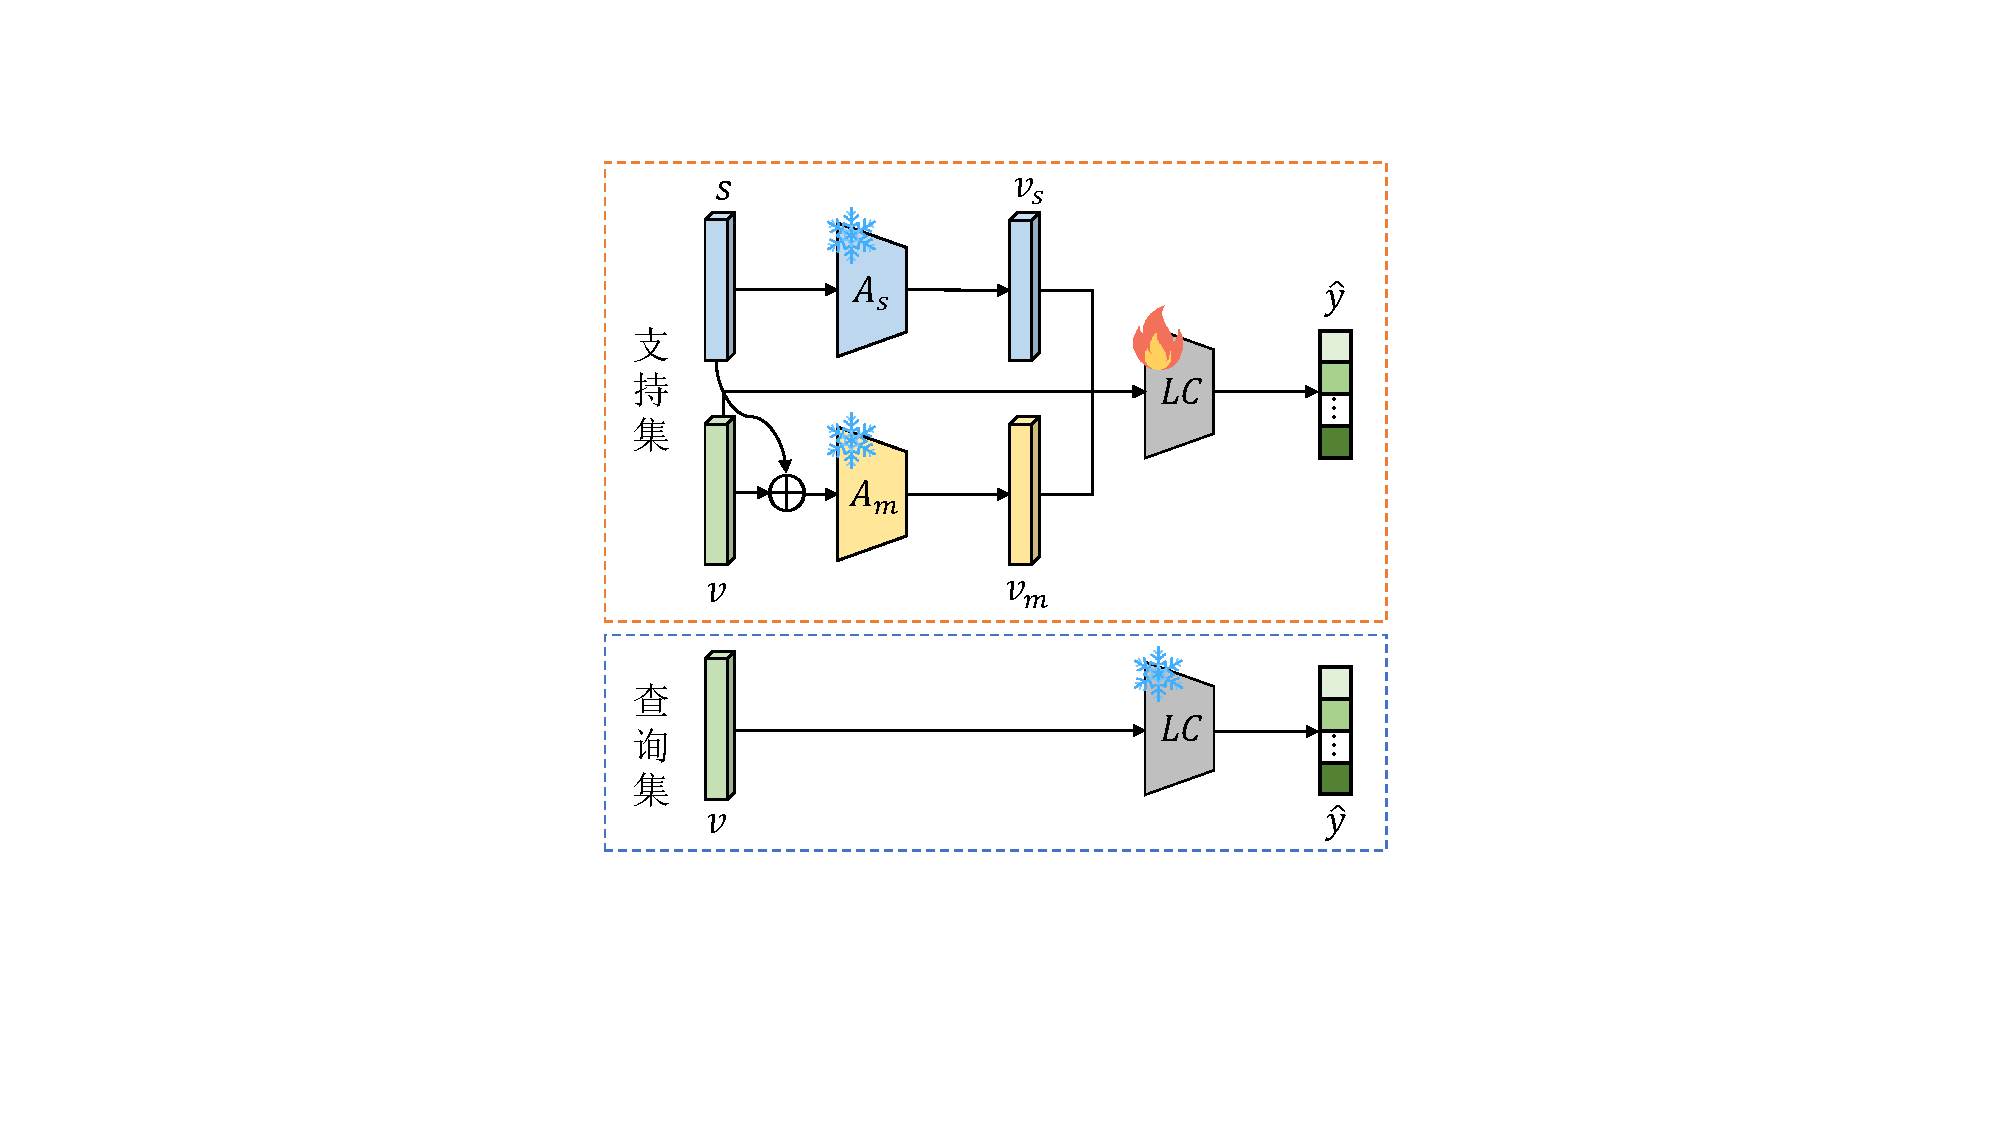
\includegraphics[width=0.6\columnwidth]{figures/SVMSMA/推理过程.pdf}
  % \captionsetup{justification=justified,singlelinecheck=false}
  \bicaption[SVMSMA模型推理过程示意图]{SVMSMA模型推理过程示意图。推理过程中,使用支持集视觉特征$v$、单模态映射特征$v_s$和多模态映射特征$v_m$训练一个逻辑回归分类器$LC$,并使用查询集视觉特征测试分类器性能。}[Illustration of SVMSMA model inference process]{Illustration of SVMSMA model inference process. During the inference process, a logistic regression classifier $LC$ is trained using the visual features $v$, single-modal mapping features $v_s$, and multi-modal mapping features $v_m$ of the support set, and the classifier's performance is tested using the visual features of the query set.}
  \label{figure4: 推理过程}
  \vspace{-7pt}
\end{figure}

\subsection[\hspace{-2pt}模型推理]{{\heiti\zihao{4} \hspace{-8pt}模型推理}}\label{section4: 模型推理}

与第三章相同,本章模型在训练完成之后,在测试阶段同样冻结所有模型参数并通过使用逻辑回归分类器$LC$执行多个少样本分类任务,将平均准确率作为模型的评价指标。不同的是,每个任务的推理过程中,本章会使用单模态映射网络$A_s$以及多模态映射网络$A_m$得到的语义映射特征$v_s$和$v_m$对原本支持集$\mathcal{S}_{\mathcal{T}}$的视觉特征$v$进行扩充,以丰富支持集样本特征的信息来源及其多样性,从而使分类器学习到更好的分类边界,达到更好的分类性能。与生成方法经常扩充支持集样本至原来的几十倍甚至上百倍不同,本文方法仅将支持集样本特征扩充至原来的3倍。对于查询集,由于无法获得其类别名称(获得类别名称相当于已知其类别),则是将其视觉特征输入训练完成的分类器$LC$获得其预测类别。本章模型推理过程如图\ref{figure4: 推理过程}所示。

\section[\hspace{-2pt}实验设置及结果分析]{{\heiti\zihao{-3} \hspace{-8pt}实验设置及结果分析}}\label{section4: 实验设置及结果分析}

在本节中,首先介绍了本章方法的实验设置,包括实验使用数据集、网络结构、以及优化设置,然后分析了基于语义-视觉多空间关系建模的少样本特征适配算法实验结果,接下来对模型的各个模块以及超参数进行了消融实验和分析,最后对模型所提取特征进行了可视化分析。

\subsection[\hspace{-2pt}实验设置]{{\heiti\zihao{4} \hspace{-8pt}实验设置}}\label{section4: 实验设置}

\textbf{(1)实验数据集介绍}

与第三章相同,本章方法同样在四个少样本分类基准数据集进行了实验,包括三个普通少样本分类数据集:miniImageNet \cite{vinyals2016matching}、tieredImageNet \cite{ren2018meta}、CIFAR-FS \cite{bertinetto2019meta},以及一个细粒度少样本分类数据集:CUB-200-2011(CUB)\cite{wah2011caltech}。不同的是,第三章方法仅使用了数据集中每个样本的图像以及标签,而本章方法还使用了数据集中包含的样本类别名称来提供语义信息。

\textbf{(2)网络结构}

在没有特殊说明的情况下,本文所使用视觉特征提取网络为第三章MGSRCL模型的特征提取网络,语义特征提取网络与SP-CLIP\cite{SP-CLIP}相同,为使用ViT-B/16架构作为图像编码器的CLIP模型的文本编码器,其输出语义特征维度为512。并且在使用CLIP模型获取语义特征时,本章方法使用了基于提示的方法,将提示文本“A photo of a”与类别名称“[class]”拼接后作为输入,如图\ref{figure4: model}所示。语义-视觉多空间映射网络则是由两层全连接,和处于两层全连接之间的ReLU激活函数组成的多层感知机。输入层维度为语义特征维度(单模态映射)或视觉特征维度和语义特征维度之和(多模态映射),隐藏层维度为4096,输出层维度为视觉特征维度。

\textbf{(3)优化设置}

对于所有实验,本文采用具有5$e^{-4}$权重衰减的自适应矩估计(Adaptive Moment Estimation,简称Adam)优化器对模型进行优化,对于tieredImageNet数据集,学习率设置为1$e^{-4}$,其余数据集均设置为1$e^{-5}$,对于所有数据集均训练100个轮次。在训练过程中,视觉特征提取网络$E_v$、语义特征提取网络$E_s$、分类器$C$参数均被冻结,只有单模态映射网络$A_s$或多模态映射网络$A_m$参与参数更新。对于超参数$\alpha$,本文在CIFAR-FS数据集将其设置为10.0,其他数据集均设置为1.0,超参数讨论将在\ref{section4: 消融实验}部分进行。

\subsection[\hspace{-2pt}基准数据集实验结果]{{\heiti\zihao{4} \hspace{-8pt}基准数据集实验结果}}\label{section4: 基准数据集实验结果}

为了评估SVMSMA模型的有效性,本文在四个数据集上进行了大量实验。模型评估过程中,同样对5-way 1-shot以及5-way 5-shot分别采样2000个任务并计算平均分类准确率作为最终实验结果。表\ref{table4: mini}、\ref{table4: tiered}、\ref{table4: CIFAR-FS}和\ref{table4: CUB}分别展示了本章方法在miniImageNet、tieredImageNet、CIFAR-FS和CUB数据集上的实验结果以及一些其他现有少样本分类方法的结果。

\textbf{(1)普通少样本分类}

与其他少样本方法相比较,本章方法SVMSMA在miniImageNet、CIFAR-FS数据集达到了最优结果,在tieredImageNet数据集达到了第二优结果,如表\ref{table4: mini}、\ref{table4: tiered}和\ref{table4: CIFAR-FS}所示。具体而言,本章提出的SVMSMA模型在miniImageNet数据集上的5-way 1-shot和5-way 5-shot任务分别达到了79.58\%和85.19\%的准确率,与第二优方法相比分别高出了7.27\%和0.79\%。在CIFAR-FS数据集,SVMSMA模型在1-shot和5-shot任务则是分别达到了86.35\%和89.42\%的准确率,比分别在1-shot和5-shot任务上达到次优结果的SP-CLIP和IER方法高出了4.17\%和0.16\%。在tieredImageNet数据集,则是SP-CLIP方法达到了最优结果,本章方法达到了第二优结果,1-shot与5-shot任务准确率分别是75.35\%和86.35\%。这些实验结果证明了本章方法的有效性。

{
\small    % 设置表格字体为5号
\setstretch{1.245}        % 设置具有指定弹力的橡皮长度(原行宽的1.2倍)
\captionsetup{font={small, stretch=1.512}}
\begin{xltabular}{\textwidth}{Clccc}
  \bilingualcaption{SVMSMA在miniImageNet数据集上的分类准确率(\%)}{SVMSMA在miniImageNet数据集上的分类准确率(\%)。最优结果用粗体表示,“Visual”与“Semantic”分别表示没有使用语义信息的方法与基于语义的方法。}{Classification accuracy (\%) of SVMSMA on miniImageNet. The best results are shown in bold, ``Visual'' and ``Semantic'' respectively refer to methods without the use of semantic information and methods based on semantic information.}
  \label{table4: mini} \\
  \toprule
  & 方法 & 特征提取网络 & 5-way 1-shot & 5-way 5-shot \\
  \midrule
  \endfirsthead

  \multicolumn{5}{c}{\tablename \thetable{} (续)} \\ % 第一行标题
  \multicolumn{5}{c}{Table \thetable{} (continued)} \\ % 第二行标题

  \toprule
  & 方法 & 特征提取网络 & 5-way 1-shot & 5-way 5-shot \\
  \midrule
  \endhead

  % \midrule \multicolumn{3}{r}{{接下页}} \\ 
  \bottomrule
  \endfoot

  \bottomrule
  \endlastfoot

  % 添加你的内容
  \multirow{14}{*}{Visual}
  & MAML \cite{MAML} & 32-32-32-32 & 48.70 $\pm$ 1.84 & 63.11 $\pm$ 0.92 \\
  & ProtoNet \cite{ProtoNet} & 64-64-64-64 & $ 49.42 \pm 0.78 $ & 68.20 $\pm$ 0.66 \\
  & DeepEMD \cite{DeepEMD} & ResNet-12 & 65.91 $\pm$ 0.82 & 82.41 $\pm$ 0.56 \\
  & RFS-distill \cite{RFS} & ResNet-12 & 64.82 $\pm$ 0.60 & 82.14 $\pm$ 0.43 \\
  % \multirow{15}{*}{Visual}
  & AssoAlign \cite{AssoAlign} & ResNet-18 & 59.88 $\pm$ 0.67 & 80.35 $\pm$ 0.73 \\
  & FEAT \cite{FEAT} & ResNet-12 & 66.78 $\pm$ 0.20 & 82.05 $\pm$ 0.14 \\
  & GIFSL \cite{GIFSL} & ResNet-12 & 65.47 $\pm$ 0.63 & 82.75 $\pm$ 0.42 \\
  & MELR \cite{MELR} & ResNet-12 & 67.40 $\pm$ 0.43 & 83.40 $\pm$ 0.28\\
  & IEPT \cite{IEPT} & ResNet-12 & 67.05 $\pm$ 0.44 & 82.90 $\pm$ 0.30 \\
  & IER \cite{IER} & ResNet-12 & 66.82 $\pm$ 0.80 & 84.35 $\pm$ 0.51 \\
  & RENet \cite{RENet} & ResNet-12 & 67.60 $\pm$ 0.44 & 82.58 $\pm$ 0.30 \\
  & PAL \cite{PAL} & ResNet-12 & 69.37 $\pm$ 0.64 & 84.40 $\pm$ 0.44 \\
  & HandCrafted \cite{HandCrafted} & ResNet-12 & 67.14 $\pm$ 0.76 & 83.11 $\pm$ 0.69 \\
  & SCL-distill \cite{Spatial} & ResNet-12 & 67.40 $\pm$ 0.76 & 83.19 $\pm$ 0.54 \\
  \multirow{8}{*}{Visual}
  & HGNN \cite{HGNN} & ResNet-12 & 67.02 $\pm$ 0.20 & 83.00 $\pm$ 0.13 \\
  & APP2S \cite{APP2S} & ResNet-18 & 64.82 $\pm$ 0.12 & 81.31 $\pm$ 0.22 \\
  & ESPT \cite{ESPT} & ResNet-12 & 68.36 $\pm$ 0.19 & 84.11 $\pm$ 0.12 \\
  & Meta-HP \cite{Meta-HP} & ResNet-12 & 62.49 $\pm$ 0.80 & 77.12 $\pm$ 0.62 \\
  & SAPENet \cite{SAPENet} & ResNet-12 & 66.41 $\pm$ 0.20 & 82.76 $\pm$ 0.14 \\
  & FEAT+DFR \cite{DFR} & ResNet-12 & 67.74 $\pm$ 0.86 & 82.49 $\pm$ 0.57 \\
  & DiffKendall \cite{DiffKendall} & ResNet-12 & 65.56 $\pm$ 0.43 & 80.79 $\pm$ 0.31 \\
  % & FGFL \cite{FGFL} & ResNet-12 & 69.14 $\pm$ 0.80 & 86.01 $\pm$ 0.62 \\
  & MetaDiff \cite{MetaDiff} & ResNet-12 & 64.99 $\pm$ 0.77 & 81.21 $\pm$ 0.56 \\
  \midrule
  \multirow{9}{*}{Semantic}
  & KTN \cite{KTN} & 64-64-128-128 & 64.42 $\pm$ 0.72 & 74.16 $\pm$ 0.56 \\
  & DualTriNet \cite{DualTriNet} & ResNet-18 & 58.12 $\pm$ 1.37 & 76.92 $\pm$ 0.69 \\
  & AM3 \cite{AM3} & ResNet-12 & 65.30 $\pm$ 0.49 & 78.10 $\pm$ 0.36 \\
  & TRAML \cite{TRAML} & ResNet-12 & 67.10 $\pm$ 0.52 & 79.54 $\pm$ 0.60 \\
  & AM3-BERT \cite{yan2021aligning} & ResNet-12 & 68.42 $\pm$ 0.51 & 81.29 $\pm$ 0.59 \\
  & CMGNN-DPGN \cite{CMGNN-DPGN} & ResNet-12 & 71.38 $\pm$ 0.51 & 82.60 $\pm$ 0.47 \\
  & STVAE \cite{STVAE} & ResNet-12 & 63.62 $\pm$ 0.80 & 80.68 $\pm$ 0.48 \\
  & SP-CLIP \cite{SP-CLIP} & Visformer-T & 72.31 $\pm$ 0.40 & 83.42 $\pm$ 0.30 \\
  \cline{2-5}
  & \raisebox{-2pt}{\textbf{SVMSMA}} & \raisebox{-2pt}{ResNet-12} & \raisebox{-2pt}{\textbf{79.58 $\pm$ 0.35}} & \raisebox{-2pt}{\textbf{85.19 $\pm$ 0.29}} \\
\end{xltabular}}


{
\small    % 设置表格字体为5号
\setstretch{1.245}        % 设置具有指定弹力的橡皮长度(原行宽的1.2倍)
\captionsetup{font={small, stretch=1.512}}
\begin{xltabular}{\textwidth}{Clccc}
  \bilingualcaption{SVMSMA在tieredImageNet数据集上的分类准确率(\%)}{SVMSMA在tieredImageNet数据集上的分类准确率(\%)。最优结果用粗体表示,带有“\dag”标记的方法表示结果是使用作者提供代码所实现,“Visual”与“Semantic”分别表示没有使用语义信息的方法与基于语义的方法。}{Classification accuracy (\%) of SVMSMA on tieredImageNet. The best results are shown in bold, and methods with the ``\dag'' indicate that the result was implemented using author-supplied code, ``Visual'' and ``Semantic'' respectively refer to methods without the use of semantic information and methods based on semantic information.}
  \label{table4: tiered} \\
  \toprule
  & 方法 & 特征提取网络 & 5-way 1-shot & 5-way 5-shot \\
  \midrule
  \endfirsthead

  \multicolumn{5}{c}{\tablename \thetable{} (续)} \\ % 第一行标题
  \multicolumn{5}{c}{Table \thetable{} (continued)} \\ % 第二行标题

  \toprule
  & 方法 & 特征提取网络 & 5-way 1-shot & 5-way 5-shot \\
  \midrule
  \endhead

  % \midrule \multicolumn{3}{r}{{接下页}} \\ 
  \bottomrule
  \endfoot

  \bottomrule
  \endlastfoot

  % 添加你的内容
  \multirow{10}{*}{Visual}
  & MAML \cite{MAML} & 32-32-32-32 & 51.67 $\pm$ 1.81 & 70.30 $\pm$ 1.75 \\
  & ProtoNet \cite{ProtoNet} & 64-64-64-64  & 53.31 $\pm$ 0.89 & 72.69 $\pm$ 0.74 \\
  & DeepEMD \cite{DeepEMD} & ResNet-12 & 71.16 $\pm$ 0.87 & 86.03 $\pm$ 0.58 \\
  & RFS-distill \cite{RFS} & ResNet-12 & 71.52 $\pm$ 0.69 & 86.03 $\pm$ 0.49 \\
  & AssoAlign \cite{AssoAlign} & ResNet-18 & 69.29 $\pm$ 0.56 & 85.97 $\pm$ 0.49 \\
  & FEAT \cite{FEAT} & ResNet-12 & 70.80 $\pm$ 0.23 & 84.79 $\pm$ 0.16 \\
  & GIFSL \cite{GIFSL} & ResNet-12 & 72.39 $\pm$ 0.66 & 86.91 $\pm$ 0.44 \\
  & MELR \cite{MELR} & ResNet-12 & 72.14 $\pm$ 0.51 & 87.01 $\pm$ 0.35 \\
  & IEPT \cite{IEPT} & ResNet-12 & 72.24 $\pm$ 0.50 & 86.73 $\pm$ 0.34 \\
  & IER \cite{IER} & ResNet-12 & 71.87 $\pm$ 0.89 & 86.82 $\pm$ 0.58 \\
  \multirow{11}{*}{Visual}
  & RENet \cite{RENet} & ResNet-12 & 71.16 $\pm$ 0.51 & 85.28 $\pm$ 0.35 \\
  & PAL \cite{PAL} & ResNet-12 & 72.25 $\pm$ 0.72 & 86.95 $\pm$ 0.47 \\
  & SCL-distill \cite{Spatial} & ResNet-12 & 71.98 $\pm$ 0.91 & 86.19 $\pm$ 0.59 \\
  & HGNN \cite{HGNN} & ResNet-12 & 72.05 $\pm$ 0.23 & 86.49 $\pm$ 0.15 \\
  & APP2S \cite{APP2S} & ResNet-18 & 70.83 $\pm$ 0.15 & 84.15 $\pm$ 0.29 \\
  & ESPT \cite{ESPT} & ResNet-12 & 72.68 $\pm$ 0.22 & 87.49 $\pm$ 0.14 \\
  & Meta-HP \cite{Meta-HP} & ResNet-12 & 68.26 $\pm$ 0.72 & 82.91 $\pm$ 0.36 \\
  & SAPENet \cite{SAPENet} & ResNet-12 & 68.63 $\pm$ 0.23 & 84.30 $\pm$ 0.16 \\
  & FEAT+DFR \cite{DFR} & ResNet-12 & 71.31 $\pm$ 0.93 & 85.12 $\pm$ 0.64 \\
  & DiffKendall \cite{DiffKendall} & ResNet-12 & 70.76 $\pm$ 0.43 & 85.31 $\pm$ 0.34 \\
  % & FGFL \cite{FGFL} & ResNet-12 & 73.21 $\pm$ 0.88 & 87.21 $\pm$ 0.61 \\
  & MetaDiff \cite{MetaDiff} & ResNet-12 & 72.33 $\pm$ 0.92 & 86.31 $\pm$ 0.62 \\
  \midrule
  \multirow{6}{*}{Semantic}
  & AM3 \cite{AM3} & ResNet-12 & 69.08 $\pm$ 0.47 & 82.58 $\pm$ 0.31 \\
  & AM3-BERT \cite{yan2021aligning} & ResNet-12 & 73.76 $\pm$ 0.72 & 87.51 $\pm$ 0.75 \\
  & CMGNN-DPGN \cite{CMGNN-DPGN} & ResNet-12 & 72.89 $\pm$ 0.49 & 84.92 $\pm$ 0.48 \\
  & STVAE\dag \cite{STVAE} & ResNet-12 & 68.32 $\pm$ 0.94 & 83.79 $\pm$ 0.66 \\
  & SP-CLIP \cite{SP-CLIP} & Visformer-T & \textbf{78.03 $\pm$ 0.46} & \textbf{88.55 $\pm$ 0.32} \\
  \cline{2-5}
  & \raisebox{-2pt}{\textbf{SVMSMA}} & \raisebox{-2pt}{ResNet-12} & \raisebox{-2pt}{75.35 $\pm$ 0.47} & \raisebox{-2pt}{86.35 $\pm$ 0.34} \\
\end{xltabular}}

{
\small    % 设置表格字体为5号
\setstretch{1.245}        % 设置具有指定弹力的橡皮长度(原行宽的1.2倍)
\captionsetup{font={small, stretch=1.512}}
\begin{xltabular}{\textwidth}{Clccc}
  \bilingualcaption{SVMSMA在CIFAR-FS数据集上的分类准确率(\%)}{SVMSMA在CIFAR-FS数据集上的分类准确率(\%)。最优结果用粗体表示,“Visual”与“Semantic”分别表示没有使用语义信息的方法与基于语义的方法。}{Classification accuracy (\%) of SVMSMA on CIFAR-FS. The best results are shown in bold, ``Visual'' and ``Semantic'' respectively refer to methods without the use of semantic information and methods based on semantic information.}
  \label{table4: CIFAR-FS} \\
  \toprule
  & 方法 & 特征提取网络 & 5-way 1-shot & 5-way 5-shot \\
  \midrule
  \endfirsthead

  \multicolumn{5}{c}{\tablename \thetable{} (续)} \\ % 第一行标题
  \multicolumn{5}{c}{Table \thetable{} (continued)} \\ % 第二行标题

  \toprule
  & 方法 & 特征提取网络 & 5-way 1-shot & 5-way 5-shot \\
  \midrule
  \endhead

  % \midrule \multicolumn{3}{r}{{接下页}} \\ 
  \bottomrule
  \endfoot

  \bottomrule
  \endlastfoot

  % 添加你的内容
  \multirow{12}{*}{Visual}
  & MAML \cite{MAML} & 32-32-32-32 & 58.90 $\pm$ 1.90 & 71.50 $\pm$ 1.00 \\
  & ProtoNet \cite{ProtoNet} & 64-64-64-64 & 55.50 $\pm$ 0.70 & 72.00 $\pm$ 0.60 \\
  & RFS-distill \cite{RFS} & ResNet-12 & 73.90 $\pm$ 0.80 & 86.90 $\pm$ 0.50  \\
  & GIFSL \cite{GIFSL} & ResNet-12 & 74.58 $\pm$ 0.38 & 87.68 $\pm$ 0.23 \\
  & IER \cite{IER} & ResNet-12 & 76.83 $\pm$ 0.82 & 89.26 $\pm$ 0.58  \\
  & RENet \cite{RENet} & ResNet-12 & 74.51 $\pm$ 0.46 & 86.60 $\pm$ 0.32  \\
  & PAL \cite{PAL} & ResNet-12 & 77.10 $\pm$ 0.70 & 88.00 $\pm$ 0.50  \\
  & HandCrafted \cite{HandCrafted} & ResNet-12 & 76.68 $\pm$ 0.59 & 87.49 $\pm$ 0.73 \\
  & SCL-distill \cite{Spatial} & ResNet-12 & 76.50 $\pm$ 0.90 & 88.00 $\pm$ 0.60  \\
  & ConstellationNet \cite{ConstellationNet} & ResNet-12 & 75.40 $\pm$ 0.20 & 86.80 $\pm$ 0.20  \\
  & APP2S \cite{APP2S} & ResNet-18 & 73.12 $\pm$ 0.22 & 85.69 $\pm$ 0.16 \\
  & Meta-HP \cite{Meta-HP} & ResNet-12 & 73.74 $\pm$ 0.57 & 86.37 $\pm$ 0.32 \\
  \midrule
  \multirow{4}{*}{Semantic}
  & DualTriNet \cite{DualTriNet} & ResNet-18 & 63.41 $\pm$ 0.64 & 78.43 $\pm$ 0.62 \\
  & STVAE \cite{STVAE} & ResNet-12 & 76.30 $\pm$ 0.60 & 87.00 $\pm$ 0.40 \\
  & SP-CLIP \cite{SP-CLIP} & Visformer-T & 82.18 $\pm$ 0.40 & 88.24 $\pm$ 0.32 \\
  \cline{2-5}
  & \raisebox{-2pt}{\textbf{SVMSMA}} & \raisebox{-2pt}{ResNet-12} & \raisebox{-2pt}{\textbf{86.35 $\pm$ 0.35}} & \raisebox{-2pt}{\textbf{89.42 $\pm$ 0.30}} \\
\end{xltabular}}

\textbf{(2)细粒度少样本分类}

同样的,本章方法也在细粒度少样本分类数据集CUB上进行了实验,结果如表\ref{table4: CUB}所示。在CUB数据集,SVMSMA模型同样取得了最优结果,在1-shot和5-shot任务上分别达到了91.17\%和94.91\%的平均准确率,比第二优的方法分别高出了5.72\%和0.18\%。这一实验证明了在类别差异较小的细粒度数据集,语义信息同样能够为视觉信息提供帮助,获得进一步性能提升。

{
\small    % 设置表格字体为5号
\setstretch{1.245}        % 设置具有指定弹力的橡皮长度(原行宽的1.2倍)
\captionsetup{font={small, stretch=1.512}}
\begin{xltabular}{\textwidth}{Clccc}
  \bilingualcaption{SVMSMA在CUB数据集上的分类准确率(\%)}{SVMSMA在CUB数据集上的分类准确率(\%)。最优结果用粗体表示,“Visual”与“Semantic”分别表示没有使用语义信息的方法与基于语义的方法。}{Classification accuracy (\%) of SVMSMA on CUB. The best results are shown in bold, ``Visual'' and ``Semantic'' respectively refer to methods without the use of semantic information and methods based on semantic information.}
  \label{table4: CUB} \\
  \toprule
  & 方法 & 特征提取网络 & 5-way 1-shot & 5-way 5-shot \\
  \midrule
  \endfirsthead

  \multicolumn{5}{c}{\tablename \thetable{} (续)} \\ % 第一行标题
  \multicolumn{5}{c}{Table \thetable{} (continued)} \\ % 第二行标题

  \toprule
  & 方法 & 特征提取网络 & 5-way 1-shot & 5-way 5-shot \\
  \midrule
  \endhead

  % \midrule \multicolumn{3}{r}{{接下页}} \\ 
  \bottomrule
  \endfoot

  \bottomrule
  \endlastfoot

  % 添加你的内容
  \multirow{12}{*}{Visual}
  % \multirow{7}{*}{Visual}
  & FEAT \cite{FEAT} & 64-64-64-64 & 68.87 $\pm$ 0.22 & 82.90 $\pm$ 0.15 \\
  & DeepEMD \cite{DeepEMD} & ResNet-12 & 75.65 $\pm$ 0.83 & 88.69 $\pm$ 0.50 \\
  & AssoAlign \cite{AssoAlign} & ResNet-18 & 74.22 $\pm$ 1.09 & 88.65 $\pm$ 0.55 \\
  & MELR \cite{MELR} & 64-64-64-64 & 70.26 $\pm$ 0.50 & 85.01 $\pm$ 0.32 \\
  & IEPT \cite{IEPT} & 64-64-64-64 & 69.97 $\pm$ 0.49 & 84.33 $\pm$ 0.33 \\
  & RENet \cite{RENet} & ResNet-12 & 79.49 $\pm$ 0.44 & 91.11 $\pm$ 0.24 \\
  & HGNN \cite{HGNN} & ResNet-12 & 78.58 $\pm$ 0.20 & 90.02 $\pm$ 0.12 \\
  & APP2S \cite{APP2S} & ResNet-12 & 77.64 $\pm$ 0.19 & 90.43 $\pm$ 0.18 \\
  & ESPT \cite{ESPT} & ResNet-12 & 85.45 $\pm$ 0.18 & 94.02 $\pm$ 0.09 \\
  & SAPENet \cite{SAPENet} & 64-64-64-64 & 70.38 $\pm$ 0.23 & 84.47 $\pm$ 0.14 \\
  & FEAT+DFR \cite{DFR} & ResNet-12 & 77.14 $\pm$ 0.21 & 88.97 $\pm$ 0.13 \\
  % & FGFL \cite{FGFL} & ResNet-12 & 80.77 $\pm$ 0.90 & 92.01 $\pm$ 0.71 \\
  & Bi-FRN \cite{Bi-FRN} & ResNet-12 & 85.44 $\pm$ 0.18 & 94.73 $\pm$ 0.09 \\
  \midrule
  \multirow{4}{*}{Semantic}
  & DualTriNet \cite{DualTriNet} & ResNet-18 & 69.61 $\pm$ 0.46 & 84.10 $\pm$ 0.35 \\
  & AM3-BERT \cite{yan2021aligning} & ResNet-12 & 77.03 $\pm$ 0.85 & 87.20 $\pm$ 0.70 \\
  & STVAE \cite{STVAE} & ResNet-12 & 77.32 $\pm$ 0.00 & 86.84 $\pm$ 0.00 \\
  \cline{2-5}
  & \raisebox{-2pt}{\textbf{SVMSMA}} & \raisebox{-2pt}{ResNet-12} & \raisebox{-2pt}{\textbf{91.17 $\pm$ 0.28}} & \raisebox{-2pt}{\textbf{94.91 $\pm$ 0.19}} \\
\end{xltabular}}

综上所述,本章提出的SVMSMA方法在miniImageNet、CIFAR-FS和CUB三个数据集达到了最优结果,在tieredImageNet数据集也达到了第二优结果,这证明了SVMSMA模型通过引入语义信息对视觉信息进行补充,使得样本特征信息来源更加丰富,从而获得更具代表性和多样性的特征,提升模型的泛化能力。另外,相比于5-way 5-shot任务,SVMSMA模型在5-way 1-shot任务取得了更为明显的效果提升,这是因为5-shot任务样本多样性已较为充足,能够使得分类器从中提取到样本关键特征进行分类,而1-shot任务样本数量较少,不足以训练一个具有良好分类边界的分类器,使用语义特征可对视觉特征进行补充,提升特征多样性,优化分类边界。

\textbf{(3)与SP-CLIP方法对比}

针对在tieredImageNet数据集上本文方法SVMSMA较SP-CLIP方法差的现象,本文猜测可能是由于SP-CLIP方法预训练网络基于Transformer架构,并且图像分辨率为224 $\times$ 244,而SVMSMA使用的预训练模型基于卷积网络架构,且图像分辨率为84 $\times$ 84。由于Transformer模型中的自注意力机制在数据集规模较大时能够更好地捕获全局信息,使其达到较卷积网络更好的结果,导致SP-CLIP在tieredImageNet数据集上能够达到更好的效果。为了验证此观点,本文使用SP-CLIP的预训练网络作为视觉特征提取网络在miniImageNet、tieredImageNet、CIFAR-FS数据集上进行了进一步实验,以在相同视觉特征提取网络与语义特征提取网络的条件下公平对比本文方法与SP-CLIP方法。

\begin{table}[h!]
  \small    % 设置表格字体为5号
  \setstretch{1.245}        % 设置具有指定弹力的橡皮长度(原行宽的1.2倍)
  \captionsetup{font={small, stretch=1.512}}
  \centering
  % \vspace{-10pt}
  \bicaption[SVMSMA与SP-CLIP的对比实验]{SVMSMA与SP-CLIP的对比实验。最优结果用粗体表示。}{Comparison of SVMSMA and SP-CLIP. The best results are shown in bold.}    % 中英文标题
  \begin{tabularx}{\textwidth}{ClCCC}
    \toprule
    数据集 & 方法      & 特征提取网络      & 5-way 1-shot              & 5-way 5-shot              \\
    \midrule
    \multirow{3}*{miniImageNet}
        & SP-CLIP & Visformer-T & 72.31 $\pm$ 0.40          & 83.42 $\pm$ 0.30          \\
        & SVMSMA   & Visformer-T & 73.51 $\pm$ 0.38          & 83.29 $\pm$ 0.32          \\
        & SVMSMA   & ResNet-12   & \textbf{79.58 $\pm$ 0.35} & \textbf{85.19 $\pm$ 0.29} \\
    \midrule
    \multirow{3}*{tieredImageNet}
        & SP-CLIP & Visformer-T & 78.03 $\pm$ 0.46          & 88.55 $\pm$ 0.32          \\
        & SVMSMA   & Visformer-T & \textbf{79.48 $\pm$ 0.44} & \textbf{88.59 $\pm$ 0.32} \\
        & SVMSMA   & ResNet-12   & 75.35 $\pm$ 0.47          & 86.35 $\pm$ 0.34          \\
    \midrule
    \multirow{3}*{CIFAR-FS}
        & SP-CLIP & Visformer-T & 82.18 $\pm$ 0.40          & 88.24 $\pm$ 0.32          \\
        & SVMSMA   & Visformer-T & 82.44 $\pm$ 0.38          & 88.32 $\pm$ 0.33          \\
        & SVMSMA   & ResNet-12   & \textbf{86.35 $\pm$ 0.35} & \textbf{89.42 $\pm$ 0.30} \\
    \bottomrule
  \end{tabularx}
  % \vspace{-25pt}
  \label{table4: comparison with SP}
\end{table}

此部分实验比较共包含三个模型,分别是SP-CLIP、使用SP-CLIP预训练网络作为视觉特征提取网络的SVMSMA(Visformer-T)、以及使用上章方法MGSRCL作为视觉特征提取网络的SVMSMA(ResNet-12),如表\ref{table4: comparison with SP}所示。实验结果显示,在5-way 1-shot任务上,SVMSMA(Visformer-T)在三个数据集上都达到了较SP-CLIP方法高的分类准确率,在miniImageNet、tieredImageNet、CIFAR-FS数据集上分别取得了1.20\%、1.45\%和0.26\%的性能提升。在5-way 5-shot任务也达到了和SP-CLIP方法相当的性能表现,仅在miniImageNet数据集准确率略微下降。这些实验结果证明了本文方法通过简单的映射网络以及损失设计便可有效利用语义信息,提升少样本分类准确率。另外,可以观察到,使用MGSRCL作为视觉特征提取网络的模型在miniImageNet、CIFAR-FS两个数据集取得了最优结果,这一现象进一步说明了第三章提到的特征学习阶段对于少样本分类的重要性。

\subsection[\hspace{-2pt}消融实验]{{\heiti\zihao{4} \hspace{-8pt}消融实验}}\label{section4: 消融实验}

\textbf{(1)讨论不同模块对模型性能的影响}

为了研究SVMSMA模型中每个模块对模型的影响,本文在miniImageNet、CIFAR-FS和CUB三个数据集上进行了消融实验,此部分实验分为四个模型,分别为基准模型(Baseline),添加跨模态分类(CMC)模块的基准模型(Baseline w/ CMC),添加跨模态特征对齐(CMFA)模块的基准模型(Baseline w/ CMFA),以及最终模型SVMSMA。此处的基准模型(Baseline)为上一章仅使用视觉信息的多粒度样本关系对比学习(MGSRCL)模型。

\begin{table}[h!]
  \small    % 设置表格字体为5号
  \setstretch{1.245}        % 设置具有指定弹力的橡皮长度(原行宽的1.2倍)
  \captionsetup{font={small, stretch=1.512}}
  \centering
  % \vspace{-10pt}
  \bicaption[SVMSMA在miniImageNet、CIFAR-FS和CUB数据集上的模块消融实验]{SVMSMA在miniImageNet、CIFAR-FS和CUB数据集上的模块消融实验。最优结果用粗体表示。}{Module ablation experiments of SVMSMA on miniImageNet, CIFAR-FS and CUB. The best results are shown in bold.}    % 中英文标题
  \begin{tabularx}{\textwidth}{ClCC}
    \toprule
    数据集 & 方法               & 5-way 1-shot              & 5-way 5-shot              \\
    \midrule
    \multirow{4}{*}{miniImageNet}
        & Baseline         & 69.57 $\pm$ 0.45          & 84.41 $\pm$ 0.30          \\
        & Baseline w/ CMC  & 76.41 $\pm$ 0.39          & 84.74 $\pm$ 0.29          \\
        & Baseline w/ CMFA & 78.82 $\pm$ 0.36          & 84.82 $\pm$ 0.29          \\
        & SVMSMA            & \textbf{79.58 $\pm$ 0.35} & \textbf{85.19 $\pm$ 0.29} \\
    \midrule
    \multirow{4}{*}{CIFAR-FS}
        & Baseline         & 78.54 $\pm$ 0.47          & 88.64 $\pm$ 0.32          \\
        & Baseline w/ CMC  & 84.18 $\pm$ 0.39          & 89.12 $\pm$ 0.31          \\
        & Baseline w/ CMFA & 85.31 $\pm$ 0.38          & 89.18 $\pm$ 0.31          \\
        & SVMSMA            & \textbf{86.35 $\pm$ 0.35} & \textbf{89.42 $\pm$ 0.30} \\
    \midrule
    \multirow{4}{*}{CUB}
        & Baseline         & 86.14 $\pm$ 0.38          & 94.75 $\pm$ 0.19          \\
        & Baseline w/ CMC  & 90.20 $\pm$ 0.30          & 94.65 $\pm$ 0.19          \\
        & Baseline w/ CMFA & 91.02 $\pm$ 0.29          & 94.65 $\pm$ 0.19          \\
        & SVMSMA            & \textbf{91.17 $\pm$ 0.28} & \textbf{94.91 $\pm$ 0.19} \\
    \bottomrule
  \end{tabularx}
  % \vspace{-25pt}
  \label{table4: module ablation}
\end{table}

在三个数据集上的模块消融实验如表\ref{table4: module ablation}所示。首先,分别添加CMC模块和CMFA模块后,模型性能较基准模型来说均有较大程度的提升,尤其是在5-way 1-shot少样本分类任务上。具体而言,添加CMC模块时,在miniImageNet、CIFAR-FS和CUB数据集1-shot任务准确率分别提升了6.84\%、5.64\%和4.06\%,添加CMFA模块时准确率分别提升了9.25\%、6.77\%和4.88\%,并且在5-shot任务上也都有小幅提升。这证明了CMC模块能够使模型将语义特征映射到视觉空间,并通过分类损失使映射后的特征与实际视觉特征具有一致性;以及CMFA模块可以使得映射后特征与类别视觉原型接近,使得样本特征更具有代表性,从而提高了分类准确率。

此外,当同时使用两个模块时,模型在三个数据集都达到了最优结果,5-way 1-shot任务准确率分别为79.58\%、86.35\%和91.17\%,5-way 5-shot任务上也同样有小幅度提升。这一现象表明了CMC模块和CMFA模块之间存在着互补性:CMC模块提供了一致性的基础,确保了映射后特征在视觉空间保持准确的语义理解;而CMFA模块进一步细化了这种理解,通过原型特征对齐使得特征更具代表性,同时优化了类内样本紧密程度。因此,通过同时使用两个模块,可以增强模型对不同类别间细微差异的识别能力,进而提高分类准确率。

\begin{figure}[h!]
  \centering
  \captionsetup{font={small, stretch=1.312}}
  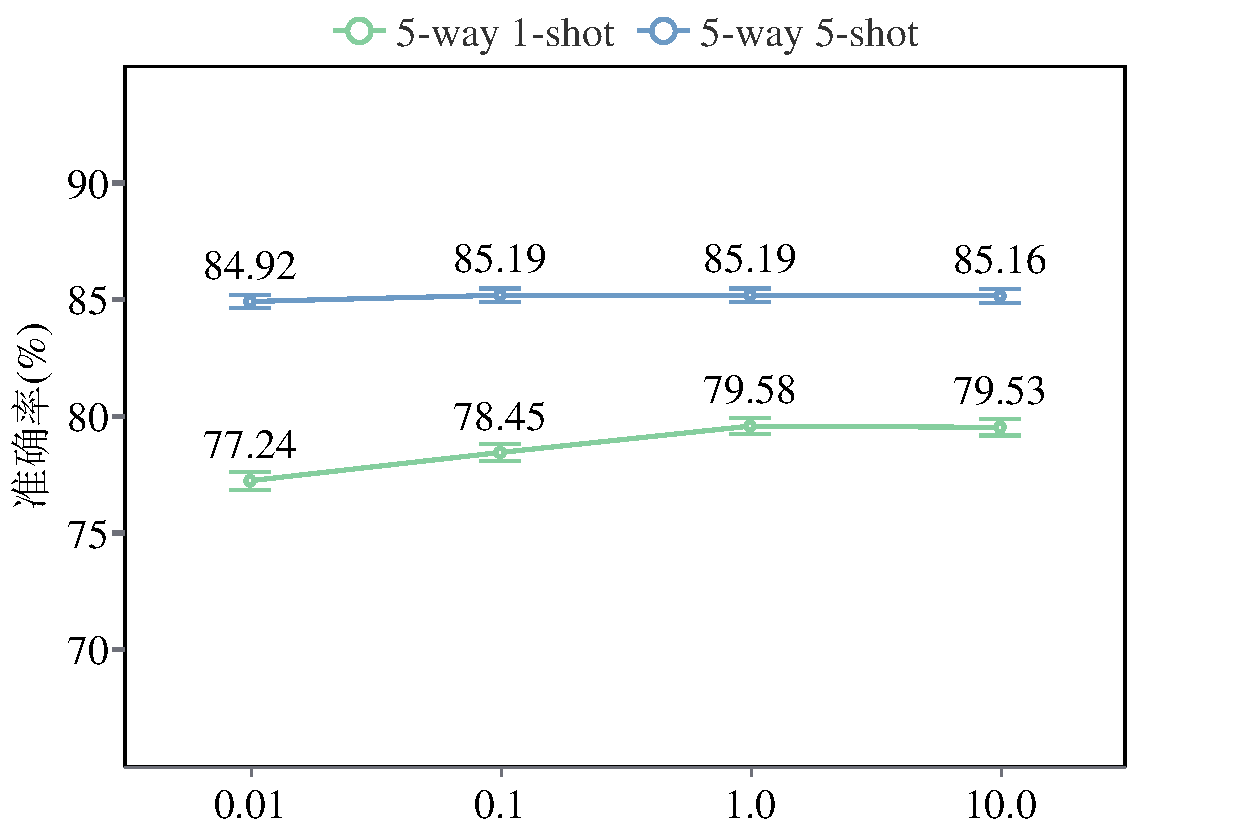
\includegraphics[width=0.6\columnwidth]{figures/SVMSMA/miniImageNet/alpha.pdf}
  \bicaption[SVMSMA在miniImageNet数据集上的超参数$\alpha$消融实验]{SVMSMA在miniImageNet数据集上的超参数$\alpha$消融实验。}[Hyperparameter $\alpha$ ablation experiments of SVMSMA on miniImageNet]{Hyperparameter $\alpha$ ablation experiments of SVMSMA on miniImageNet.}
  \label{figure4: alpha (miniImageNet)}
  % \vspace{-4pt}
\end{figure}

\begin{figure}[h!]
  \centering
  \captionsetup{font={small, stretch=1.312}}
  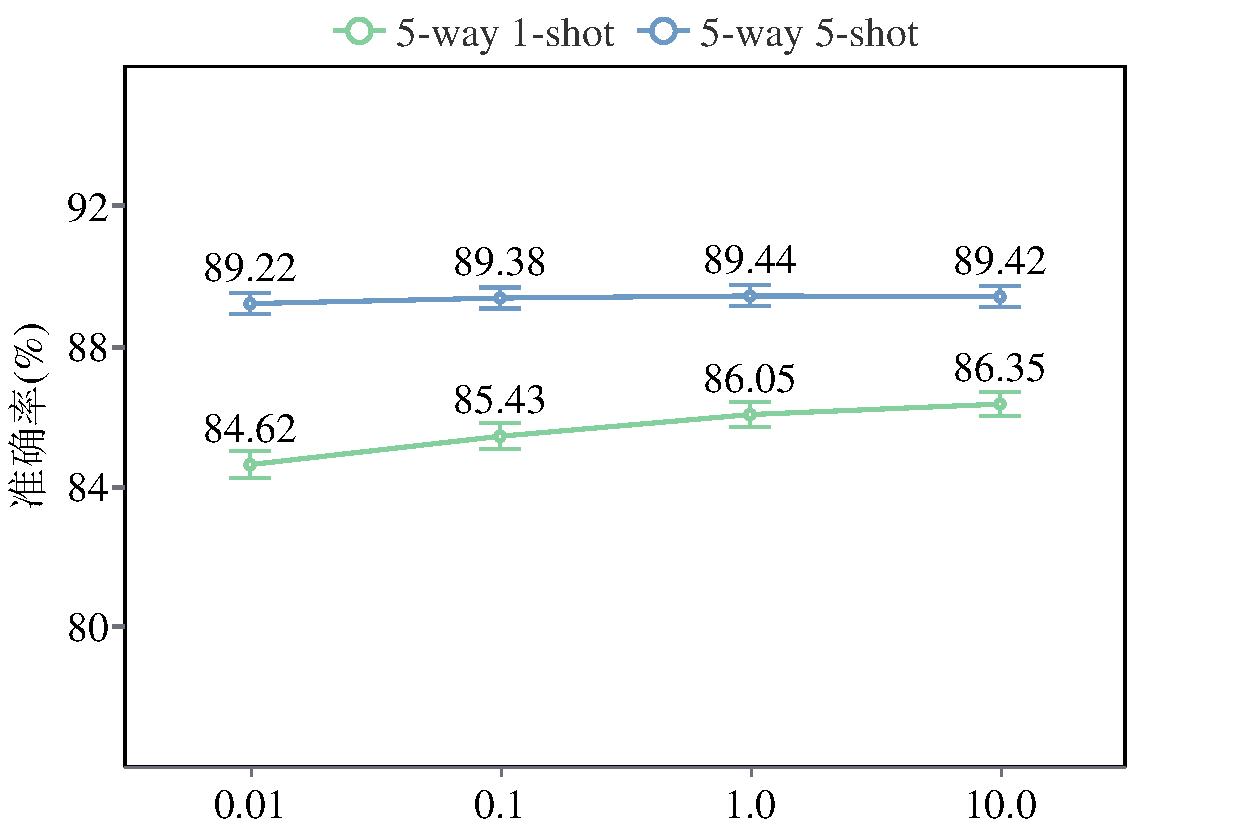
\includegraphics[width=0.6\columnwidth]{figures/SVMSMA/CIFAR-FS/alpha.pdf}
  \bicaption[SVMSMA在CIFAR-FS数据集上的超参数$\alpha$消融实验]{SVMSMA在CIFAR-FS数据集上的超参数$\alpha$消融实验。}[Hyperparameter $\alpha$ ablation experiments of SVMSMA on CIFAR-FS]{Hyperparameter $\alpha$ ablation experiments of SVMSMA on CIFAR-FS.}
  \label{figure4: alpha (CIFAR-FS)}
  % \vspace{-4pt}
\end{figure}

\begin{figure}[h!]
  \centering
  \captionsetup{font={small, stretch=1.312}}
  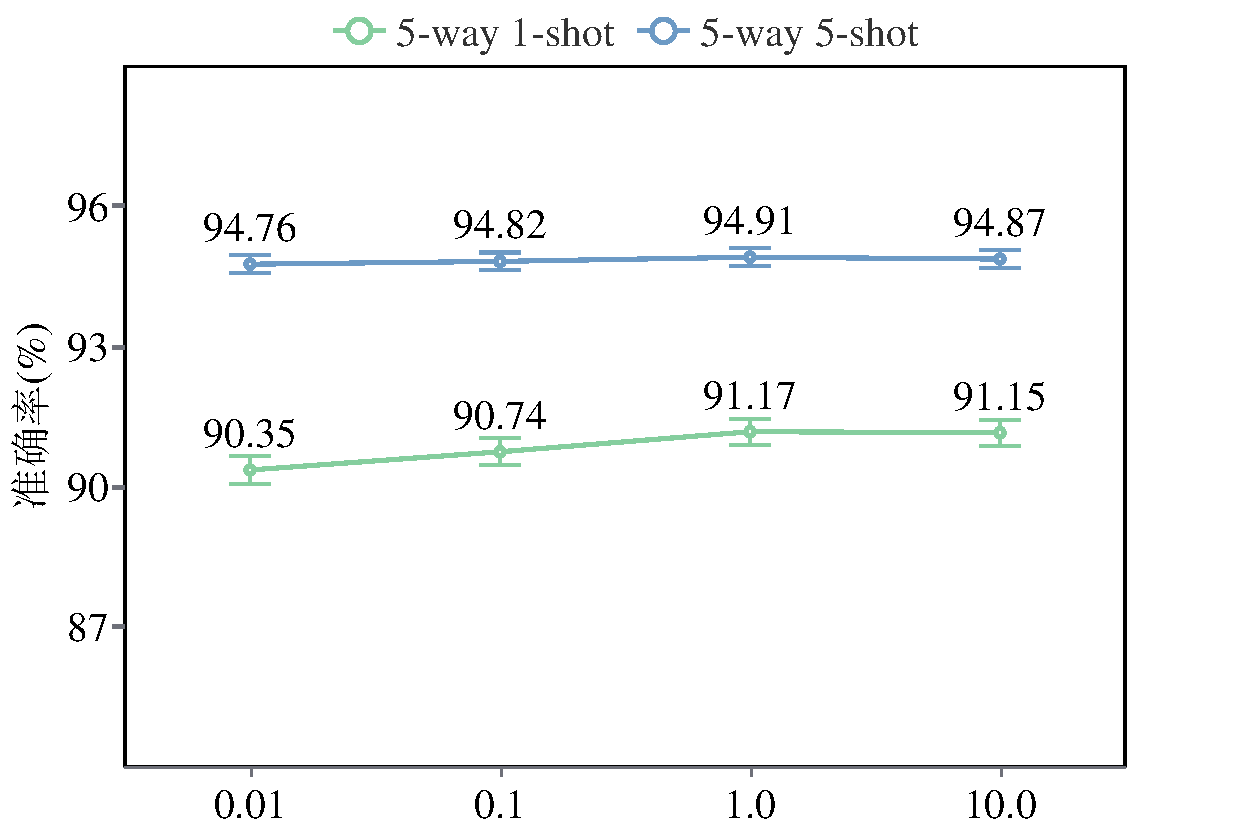
\includegraphics[width=0.6\columnwidth]{figures/SVMSMA/CUB/alpha.pdf}
  \bicaption[SVMSMA在CUB数据集上的超参数$\alpha$消融实验]{SVMSMA在CUB数据集上的超参数$\alpha$消融实验。}[Hyperparameter $\alpha$ ablation experiments of SVMSMA on CUB]{Hyperparameter $\alpha$ ablation experiments of SVMSMA on CUB.}
  \label{figure4: alpha (CUB)}
  % \vspace{-4pt}
\end{figure}

\textbf{(2)讨论超参数对模型性能的影响}

$\alpha$是调整不同损失权重占比的超参数,本文通过将其设置为不同数值来讨论$\alpha$对模型的影响,同样在miniImageNet、CIFAR-FS、CUB三个数据集进行了实验分析。

如图\ref{figure4: alpha (miniImageNet)}、\ref{figure4: alpha (CIFAR-FS)}和\ref{figure4: alpha (CUB)}所示,对于miniImageNet和CUB数据集,无论是5-way 1-shot还是5-way 5-shot任务,模型均在将$\alpha$设置为1.0时达到最优结果,因此对于这两个数据集,$\alpha$被设置为1.0。而对于CIFAR-FS数据集,5-way 1-shot任务在$\alpha = 10.0$时取得最优结果,5-way 5-shot任务则是在$\alpha = 1.0$取得最优结果,但5-shot任务准确率差别很微小,因此在CIFAR-FS数据集上,超参数$\alpha$被设置为10.0。此外,超参数$\alpha$被设置为0.1、1.0与10.0时,模型结果变化较小,这证明了所提方法对超参数$\alpha$的稳定性。

\begin{table}[h!]
  \small    % 设置表格字体为5号
  \setstretch{1.245}        % 设置具有指定弹力的橡皮长度(原行宽的1.2倍)
  \captionsetup{font={small, stretch=1.512}}
  \centering
  % \vspace{-10pt}
  \bicaption[SVMSMA在miniImageNet、CIFAR-FS和CUB数据集上的不同特征消融实验]{SVMSMA在miniImageNet、CIFAR-FS和CUB数据集上的不同特征消融实验。最优结果用粗体表示。}{Different features ablation experiments of SVMSMA on miniImageNet, CIFAR-FS and CUB. The best results are shown in bold.}    % 中英文标题
  \begin{tabularx}{\textwidth}{ClCC}
    \toprule
    数据集 & 特征      & 5-way 1-shot              & 5-way 5-shot              \\
    \midrule
    \multirow{4}{*}{miniImageNet}
        & 视觉特征    & 69.57 $\pm$ 0.45          & 84.41 $\pm$ 0.30          \\
        & 单模态映射特征 & 73.73 $\pm$ 0.39          & 73.83 $\pm$ 0.39          \\
        & 多模态映射特征 & 78.34 $\pm$ 0.37          & 81.29 $\pm$ 0.34          \\
        & SVMSMA   & \textbf{79.58 $\pm$ 0.35} & \textbf{85.19 $\pm$ 0.29} \\
    \midrule
    \multirow{4}{*}{CIFAR-FS}
        & 视觉特征    & 78.54 $\pm$ 0.47          & 88.64 $\pm$ 0.32          \\
        & 单模态映射特征 & 83.44 $\pm$ 0.37          & 83.60 $\pm$ 0.38          \\
        & 多模态映射特征 & 86.00 $\pm$ 0.36          & 87.40 $\pm$ 0.33          \\
        & SVMSMA   & \textbf{86.35 $\pm$ 0.35} & \textbf{89.42 $\pm$ 0.30} \\
    \midrule
    \multirow{4}{*}{CUB}
        & 视觉特征    & 86.14 $\pm$ 0.38          & 94.75 $\pm$ 0.19          \\
        & 单模态映射特征 & 83.58 $\pm$ 0.43          & 83.53 $\pm$ 0.43          \\
        & 多模态映射特征 & 89.90 $\pm$ 0.31          & 93.60 $\pm$ 0.22          \\
        & SVMSMA   & \textbf{91.17 $\pm$ 0.28} & \textbf{94.91 $\pm$ 0.19} \\
    \bottomrule
  \end{tabularx}
  % \vspace{-25pt}
  \label{table4: modal ablation}
\end{table}

\textbf{(3)讨论不同映射模式特征的分类准确率}

如\ref{section4: 语义-视觉多空间映射网络}所述,根据映射网络输入特征模态不同,可将其分为两种模式:单模态映射和多模态映射。为讨论不同映射模式特征对少样本分类结果的影响,本文进行了实验分析。

如表\ref{table4: modal ablation}所示,对于5-way 1-shot任务,无论是单模态映射特征,还是多模态映射特征,均取得了较视觉特征高的准确率。这证明了利用语义特征可以更好地建立新类与基类之间联系,从而迁移在基类上学习到的知识,也证明了语义信息对少样本分类的重要性。另外,在将三个特征共同作为分类器的训练数据时,模型能够取得进一步的效果提升。对于5-way 5-shot任务,相对于视觉特征,单模态映射特征和多模态映射特征的准确率均有所降低,尤其是单模态映射特征,降低幅度尤为明显。导致这种现象出现的原因是因为每个类别的语义特征以及视觉原型特征都是固定的,将其映射到视觉空间并执行分类与特征对齐任务会使其得模型学习到一个投影相对固定的映射网络,即映射后特征的多样性会较差。因此即使其更接近类别中心,但由于多样性差会导致其不如使用多样性较好的视觉特征训练出来的分类边界更加鲁棒,导致取得较差的5-shot任务结果。虽然多模态映射模式中将视觉特征与语义特征共同输入网络缓解了这种情况,但仍比视觉特征的分类准确率低。本文通过使用三种特征一起训练分类器,利用视觉特征的多样性解决了此问题,取得了较使用单一特征更好的结果。


\begin{table}[h!]
  \small    % 设置表格字体为5号
  \setstretch{1.245}        % 设置具有指定弹力的橡皮长度(原行宽的1.2倍)
  \captionsetup{font={small, stretch=1.512}}
  \centering
  % \vspace{-10pt}
  \bicaption[SVMSMA在miniImageNet、CIFAR-FS和CUB数据集上的不同语义特征消融实验]{SVMSMA在miniImageNet、CIFAR-FS和CUB数据集上的不同语义特征消融实验。最优结果用粗体表示。}{Different semantic features ablation experiments of SVMSMA on miniImageNet, CIFAR-FS and CUB. The best results are shown in bold.}    % 中英文标题
  \begin{tabularx}{\textwidth}{ClCC}
    \toprule
    数据集 & 方法                 & 5-way 1-shot              & 5-way 5-shot              \\
    \midrule
    \multirow{4}{*}{miniImageNet}
        & Baseline           & 69.57 $\pm$ 0.45          & 84.41 $\pm$ 0.30          \\
        & SVMSMA-GloVe (name) & 71.53 $\pm$ 0.46          & 81.49 $\pm$ 0.34          \\
        & SVMSMA-SBERT (name) & 73.29 $\pm$ 0.43          & 82.94 $\pm$ 0.32          \\
        & SVMSMA-CLIP (name)  & 78.16 $\pm$ 0.37          & 84.93 $\pm$ 0.28          \\
        & SVMSMA-CLIP (text)  & \textbf{79.58 $\pm$ 0.35} & \textbf{85.19 $\pm$ 0.29} \\
    \midrule
    \multirow{4}{*}{CIFAR-FS}
        & Baseline           & 78.54 $\pm$ 0.47          & 88.64 $\pm$ 0.32          \\
        & SVMSMA-GloVe (name) & 83.19 $\pm$ 0.40          & 88.25 $\pm$ 0.32          \\
        & SVMSMA-SBERT (name) & 82.24 $\pm$ 0.41          & 88.15 $\pm$ 0.31          \\
        & SVMSMA-CLIP (name)  & 85.34 $\pm$ 0.37          & 89.24 $\pm$ 0.30          \\
        & SVMSMA-CLIP (text)  & \textbf{86.35 $\pm$ 0.35} & \textbf{89.42 $\pm$ 0.30} \\
    \midrule
    \multirow{4}{*}{CUB}
        & Baseline           & 86.14 $\pm$ 0.38          & 94.75 $\pm$ 0.19          \\
        & SVMSMA-GloVe (name) & 87.67 $\pm$ 0.35          & 93.83 $\pm$ 0.21          \\
        & SVMSMA-SBERT (name) & 87.40 $\pm$ 0.35          & 94.20 $\pm$ 0.20          \\
        & SVMSMA-CLIP (name)  & 91.06 $\pm$ 0.28          & \textbf{94.91 $\pm$ 0.19} \\
        & SVMSMA-CLIP (text)  & \textbf{91.17 $\pm$ 0.28} & \textbf{94.91 $\pm$ 0.19} \\
    \bottomrule
  \end{tabularx}
  \label{table4: text encoder ablation}
\end{table}

\textbf{(4)讨论不同语义特征提取网络对模型性能的影响}

为了进一步证明本文方法的可推广性,本文也使用其他模型作为语义特征提取网络:GloVe与SBERT,对于这两个模型,本文使用类别名称作为模型的输入,因此表示为SVMSMA-GloVe (name)与SVMSMA-SBERT (name)。

如表\ref{table4: text encoder ablation}所示,在1-shot任务上,SVMSMA-GloVe与SVMSMA-SBERT都通过提高样本特征多样性的手段取得了优于基准模型的表现,从而进一步证明了语义特征对于少样本分类问题的重要性以及本文方法的可迁移性。而在5-shot任务上,模型性能均有所降低,尤其是在miniImageNet数据集上。这是因为这两个模型提取的语义特征迁移性不够好,语义映射特征并不像使用CLIP模型时具有代表性,原本较多数量的视觉特征便可以使分类器学习到良好分类边界,而增加了这些样本会对样本特征空间造成一定的干扰,使其偏离原本分类边界,且为向远离真实分类边界的方向偏离,造成性能下降。虽说通过调整各种特征的比例能够缓解或避免这种现象,但为了方法的简易性,对此部分内容本文不再进行描述。

此外,本文也讨论了是否使用提示文本对模型性能的影响,使用类别名称作为CLIP文本编码器输入进行了实验。使用类别名称作为输入时,模型表示为SVMSMA-CLIP (name),添加提示文本时则表示为SVMSMA-CLIP (text),如表\ref{table4: text encoder ablation}所示。可以观察到,虽然SVMSMA-CLIP (name)模型也取得了优异的效果,但仍不如添加提示文本后模型表现,在miniImageNet、CIFAR-FS和CUB三个数据集1-shot任务上分别降低了1.42\%、1.01\%和0.11\%的准确率,在5-shot任务也有略微降低。这一实验证明了提示文本对模型表现具有一定影响,也为将来通过设计提示文本或将其参数化进一步提升模型性能提供了依据。

\begin{figure}[h!]
  \centering
  \captionsetup{font={small, stretch=1.312}}
  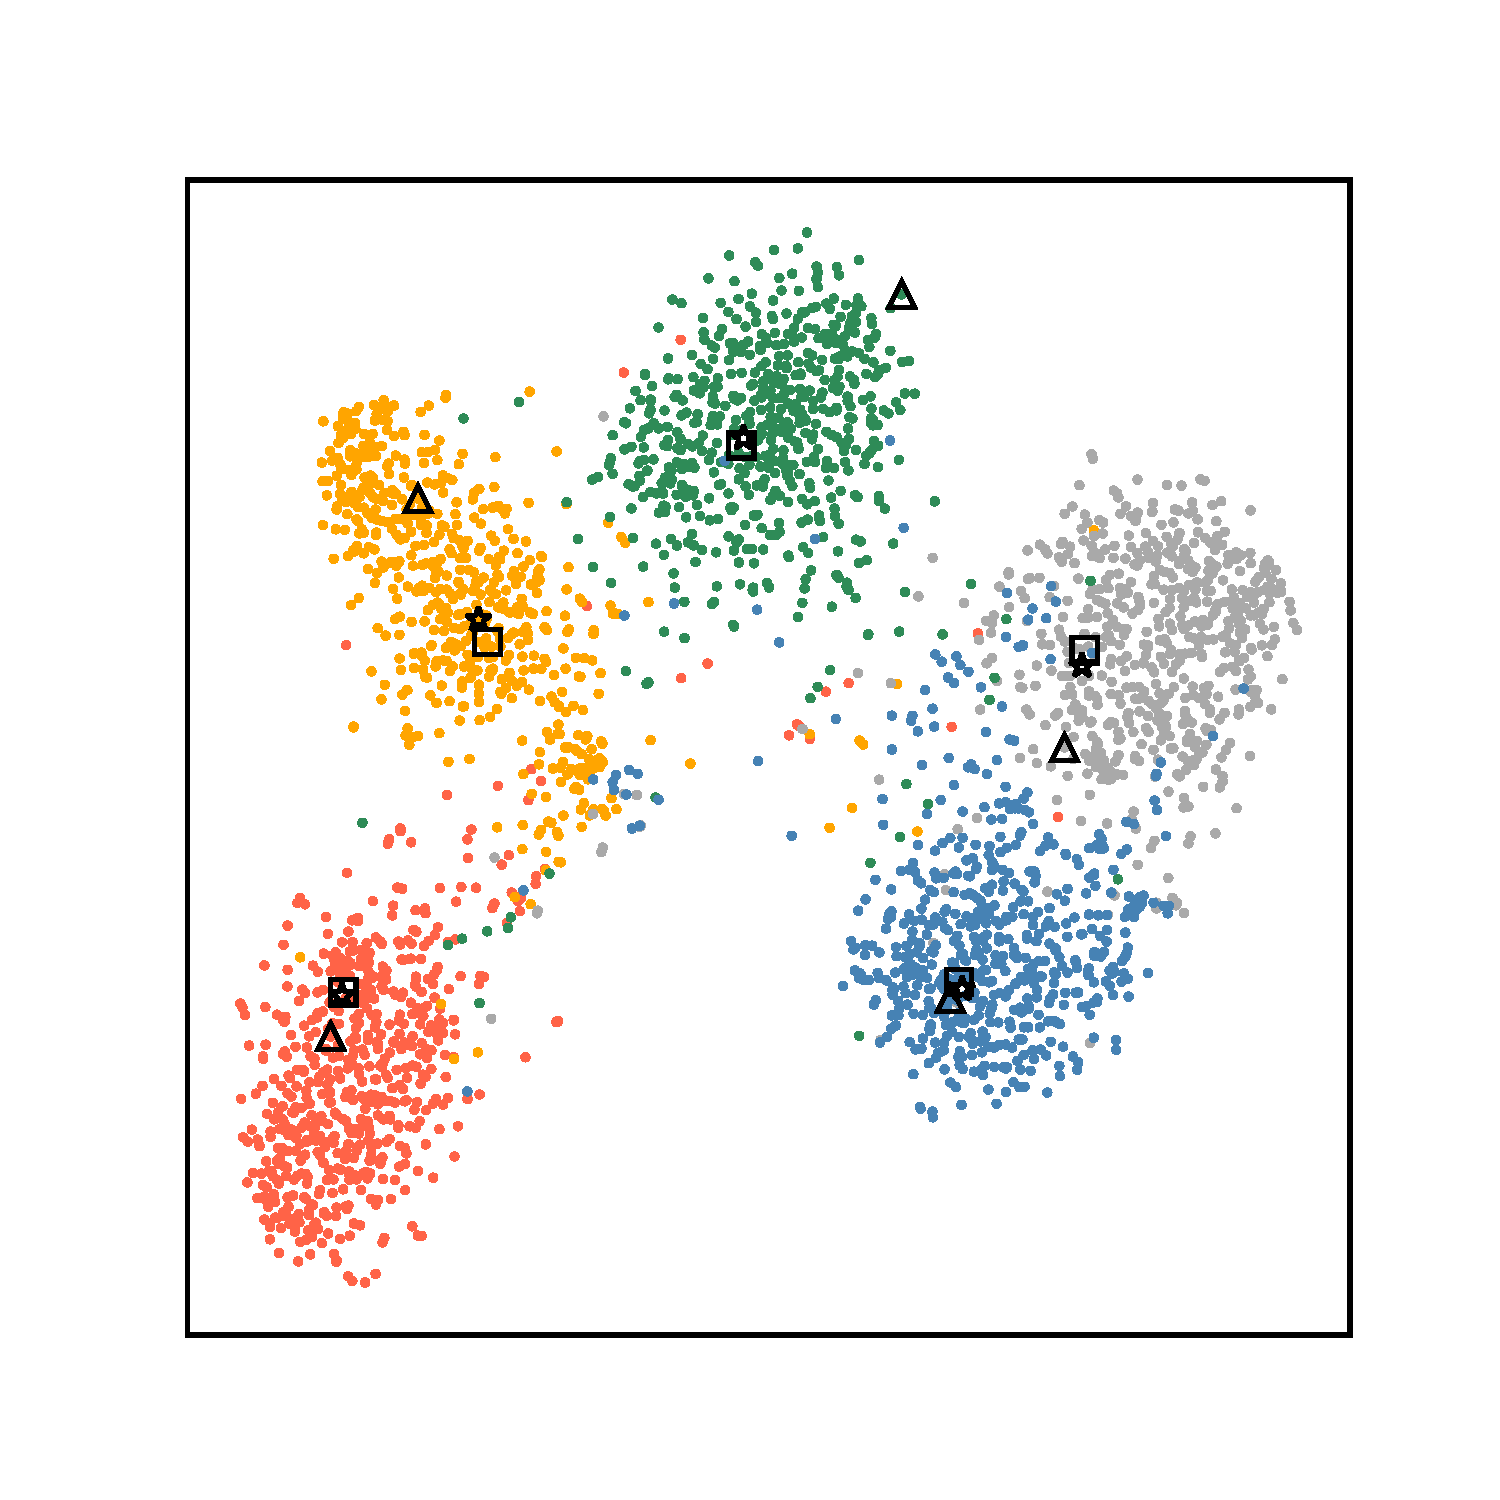
\includegraphics[width=0.5\columnwidth]{figures/SVMSMA/miniImageNet/t-SNE.pdf}
  \bicaption[miniImageNet数据集上不同特征的t-SNE可视化结果]{miniImageNet数据集上不同特征的t-SNE可视化结果。不同颜色代表不同类别。视觉特征、单模态映射特征、多模态映射特征分别用$\triangle$、$\Box$和$\hollowstar$表示。}[The t-SNE visualization results of different features on miniImageNet]{The t-SNE visualization results of different features on miniImageNet. Different colors represent different categories. visual features, single-modal mapping features, and multi-modal mapping features are represented by $\triangle$, $\Box$, and $\hollowstar$, respectively.}
  \label{figure4: t-SNE}
\end{figure}

\subsection[\hspace{-2pt}可视化分析]{{\heiti\zihao{4} \hspace{-8pt}可视化分析}}\label{section4: 可视化分析}

为了更好地展示SVMSMA方法能够通过引入语义特征对视觉特征进行补充,本文在miniImageNet数据集上随机选取了5个新类并使用t-SNE对每个类别所有样本的视觉特征,随机选取一个5-way 1-shot任务支持集样本的视觉特征($\triangle$)、单模态映射特征($\Box$)、多模态映射特征($\hollowstar$)进行了可视化实验,如图\ref{figure4: t-SNE}所示。在此图里,可以看到无论是单模态特征还是多模态特征都能较好地落在样本簇中,这使得将它们加入逻辑回归器的训练数据可以提升支持集样本特征的多样性,从而在查询集上达到更好的分类效果。另外,在某些较为极端的情况下,如图中绿色类别和灰色类别所示,支持集样本视觉特征处于类别边缘或者分类边界。对于这种情况,如果单独使用视觉特征一般会取得较差的分类结果。而使用本文提出方法所获取的单模态映射特征和多模态映射特征则处于样本簇较为中央的位置,从而能够校正视觉特征造成的偏差,优化分类器学习到的分类边界,达到更好的准确率。综上所述,SVMSMA方法能够使用语义信息对视觉信息进行补充,通过增加支持集样本的方式丰富支持集样本的多样性,同时对视觉特征处于样本簇边缘时造成的分类边界偏差进行修正,从而提高少样本分类任务的准确率。


\section[\hspace{-2pt}本章小结]{{\heiti\zihao{-3} \hspace{-8pt}本章小结}}\label{section4: 本章小结}

本章研究基于语义-视觉多空间关系建模的少样本特征适配算法,针对少样本分类中仅根据少量视觉特征无法捕获类别代表性特征的缺点,引入语义信息作为视觉信息的补充,通过对语义-视觉多空间关系进行建模,提出了语义-视觉多空间映射适配模型(Semantic-Visual Multi-Space Mapping Adapter,简称SVMSMA),以丰富样本特征的信息来源,利用语义特征对视觉特征进行补充与修正,从而提升模型在新类上的泛化能力。SVMSMA模型使用单/多模态映射网络将样本语义特征映射到视觉空间获得单/多模态映射特征,并通过跨模态分类(CMC)模块与跨模态特征对齐(CMFA)模块对映射网络进行优化,以使得语义特征与视觉特征建立联系。测试过程中,本章方法将支持集的视觉特征、单模态映射特征、以及多模态映射特征共同作为分类器的训练数据,达到了较仅使用单一特征时更好的分类结果。在miniImageNet、tieredImageNet、CIFAR-FS和CUB-200-2011数据集的大量实验表明了SVMSMA方法的有效性。

综上所述,本章提出的基于语义-视觉多空间关系建模的少样本特征适配算法通过对语义-视觉多空间关系进行建模,充分利用语义信息对视觉信息进行了补充,丰富了样本特征信息来源,提升了模型的泛化能力。

\chapter[\hspace{0pt}总结与未来展望]{{\heiti\zihao{3}\hspace{0pt}总结与未来展望}}\label{section 7}
\removelofgap
\removelotgap

本章内容共分为两节,\hyperref[section5: 总结]{第一节}对本文研究内容与方法进行总结;\hyperref[section5: 未来展望]{第二节}介绍本文所提方法的局限性并对未来研究方向进行展望。

\section[\hspace{-2pt}总结]{{\heiti\zihao{-3} \hspace{-8pt}总结}}\label{section5: 总结}

少样本分类致力于模拟人类的知识迁移能力,期望模型在具有大量标注数据的基类数据上训练之后,能够将所学知识迁移至新类别,实现用少量标注样本进行有效学习。目前,少样本分类问题已取得一系列研究成果,但仍存在一些问题与挑战:特征提取网络迁移能力不够强;样本数量极少情况下无法捕获类别代表性特征。针对这些问题,本文分别从多粒度样本关系建模与语义-视觉多空间关系建模两个角度出发,对少样本分类中的多元关系进行了深入挖掘与研究。

(1)本文首先从多粒度样本关系建模的角度出发,开展了基于多粒度样本关系建模的少样本分类研究。针对少样本分类模型特征提取能力不足的问题,提出了一种基于多粒度样本关系对比学习的少样本特征学习算法:多粒度样本关系对比学习(Multi-Grained Sample Relation Contrastive Learning,简称MGSRCL)模型,旨在通过对不同粒度的样本关系进行建模以提升模型的特征提取能力。MGSRCL使用变换一致性学习来约束同一样本不同变换版本之间的样本内关系,通过使其预测概率分布相同令它们在语义内容上保持一致;使用类对比学习来约束同类样本的类内关系和不同类样本的类间关系,通过对其特征进行建模使同类样本语义内容相似、不同类样本语义内容不同。通过对多种粒度的样本关系细致地建模,MGSRCL提升了模型的特征提取能力,达到了优异的少样本分类结果。在miniImageNet、tieredImageNet、CIFAR-FS和CUB四个少样本基准数据集上的大量实验证明了MGSRCL的有效性。另外,通过将MGSRCL模型作为预训练模型与其他方法结合,证明了所获得特征提取网络的可迁移性。

(2)上述提出的MGSRCL方法虽然达到了优异的结果,但仍存在没有利用样本语义信息的问题。因此,以MGSRCL方法为基础,本文进一步进行了基于语义-视觉多空间关系建模的少样本分类研究。针对少量样本的视觉特征无法捕获类别代表性特征的问题,提出了一种基于语义-视觉多空间关系建模的少样本特征适配算法:语义-视觉多空间映射适配(Semantic-Visual Multi-Space Mapping Adapter,简称SVMSMA)模型,旨在引入语义信息对视觉信息进行补充,丰富样本特征的信息来源以提升其多样性与代表性。SVMSMA使用语义-视觉多空间映射网络将语义特征映射到视觉空间,并通过跨模态分类模块对单/多模态映射特征执行分类任务使其与视觉特征建立联系,以及跨模态特征对齐模块将映射特征与视觉特征原型进行对齐以获得更接近类别原型的特征。通过对语义-视觉多空间关系进行建模,SVMSMA丰富了样本特征的信息来源,提升了模型的泛化能力。在四个基准数据集上的实验证明了SVMSMA方法能够有效利用语义信息,在MGSRCL的基础上进一步提升少样本分类结果。

本文使用MGSRCL模型和SVMSMA模型分别对数据间的多种样本关系以及多种空间映射关系进行了建模,有效利用了数据中的多元关系,通过多粒度样本关系建模提升了视觉特征提取网络的特征提取能力,通过语义-视觉多空间关系建模提升了模型的泛化能力,从而取得了较好的少样本分类结果。

\section[\hspace{-2pt}未来展望]{{\heiti\zihao{-3} \hspace{-8pt}未来展望}}\label{section5: 未来展望}

本文分析了少样本分类面临的挑战,以数据中的多元关系为切入点,从多粒度样本关系建模与语义-视觉多空间建模两个角度入手,提出了多粒度样本关系对比学习模型和语义-视觉多空间映射适配模型来解决少样本分类问题,并取得了一定成果。但仍存在一定不足,后续可从以下几方面进一步研究:

(1)本文提出的MGSRCL方法中产生变换样本时使用的多是一些弱数据增强方法,其对特征提取网络性能提升产生的作用较为有限。目前诸如Mixup、CutMix、以及AugMix等强数据增强已被证明了能够提高模型泛化能力,但由于其会将不同图像融合形成一张新的图像,这使得图像类别不再是单一标签,无法应用于MGSRCL。因此,后续工作可以探讨如何将强数据增强方法引入所提出的方法,或者对方法进行改进以提高其适用性。

(2)本文通过使用CLIP模型的文本编码器作为语义特征提取网络,引入语义信息对视觉信息进行补充并取得了优异结果。在将类别名称输入文本编码器时,使用了CLIP原论文中提出的提示文本。但使用的提示文本是固定的,并不一定能够让模型输出对少样本分类任务来说最优的语义特征。因此后续可进一步研究其他提示文本或者将提示文本换成可学习参数,以获取最优的语义特征。

(3)本文中特征提取网络使用卷积网络,并没有使用近年来在很多视觉任务上取得良好表现的Transformer模型。这是因为Transformer模型一般需要大量的数据才能得到一个具有强大特征提取能力的预训练模型,而在少样本分类任务中,仅有tieredImageNet数据集规模较大,因此如何将Transformer模型引入少样本分类任务并取得像在其他任务上超越卷积网络的效果也是后续研究方向之一。
%\include{contents/yourFreeChoise}

\backmatter %%% 后置部分(致谢、参考文献、附录等)

%% 参考文献
% 顺序编码制:cqunumerical		
% 注意:至少需要引用一篇参考文献,否则下面两行会引起编译错误。
% \bibliographystyle{cqunumerical}
\bibliographystyle{gbt7714-numerical_new}
\bibliography{ref/refs}


%% 附录(按ABC...分节,证明、推导、程序、个人简历等)
\appendix
\chapter[附\hskip\ccwd{}\hskip\ccwd{}录]{{\heiti\zihao{3}附\hskip\ccwd{}\hskip\ccwd{}录}}

\section[\hspace{-2pt}作者在攻读硕士学位期间的论文目录]{{\heiti\zihao{-3} \hspace{-8pt}作者在攻读硕士学位期间的论文目录}}

%下面是盲审标记\cs{secretize}的用法,记得去\textsf{main.tex}开启盲审开关看效果:

% \circled{1}已发表论文

% \begin{enumerate}
%     \item \textbf{\secretize{XU X}}, \secretize{LIU K}, DAI P, et al. Joint task offloading and resource optimization in NOMA-based vehicular edge computing: A game-theoretic DRL approach[J]. Journal of Systems Architecture, 2023, 134: 102780. 影响因子: 5.836(2021), 4.497(5年) (中科院SCI 2区,对应本文第三章)
% 	\item \textbf{\secretize{许新操}}, \secretize{刘凯}, 刘春晖, 等. 基于势博弈的车载边缘计算信道分配方法[J]. 电子学报, 2021,49(5): 851-860. (EI 索引,CCF T1类中文高质量科技期刊,对应本文第三章)
% 	\item \textbf{ \secretize{XU X}}, \secretize{LIU K}, XIAO K, et al. Vehicular fog computing enabled real-time collision warning via trajectory calibration[J]. Mobile Networks and Applications, 2020, 25(6): 2482-2494. 影响因子: 3.077(2021), 2.92(5年) (中科院SCI 3区,对应本文第五章)
% \end{enumerate}
{
\small
\setlength{\baselineskip}{20pt}
\begin{enumerate}[label={[\arabic*]}, leftmargin=*]
\item {\secretize{Yin G}}, \secretize{Huang S}, He T, et al. Mirrored EAST: An Efficient Detector for Automatic Vehicle Identification Number Detection in the Wild[J]. IEEE Transactions on Industrial Informatics, 2023. (中科院SCI一区)
\item {\secretize{Yin G}}, Wang Y, Zhang Y, et al. Adversarial Bidirectional Feature Generation for Generalized Zero-Shot Learning Under Unreliable Semantics[C]//Chinese Conference on Pattern Recognition and Computer Vision (PRCV). Cham: Springer Nature Switzerland, 2022: 639-654.(CCF-C)
\item {\secretize{Yin G}}, Huangfu L, \secretize{Huang S}, et al. Rethinking the Sample Relations for Few-Shot Classification[J]. Image and Vision Computing. (中科院SCI三区,返修中)
\end{enumerate}
}


\section[\hspace{-2pt}作者在攻读硕士学位期间参与的科研项目]{{\heiti\zihao{-3} \hspace{-8pt}作者在攻读硕士学位期间参与的科研项目}}

{
\small
\setlength{\baselineskip}{20pt}
\begin{enumerate}[label={[\arabic*]}, leftmargin=*]
\item 国家自然科学基金面上项目,少样本学习特征生成与鲁棒性关键技术研究
% (No. 62176030)
\item 重庆市自然科学基金面上项目,文本描述协同的双向生成式少样本学习研究
\end{enumerate}
}

% \newpage
% \section[\hspace{-2pt}学位论文数据集]{{\heiti\zihao{-3} \hspace{-8pt}学位论文数据集}}

% \begin{table}[h]
% \resizebox{\columnwidth}{!}{%
% \begin{tabular}{|cllcclclcl|}
% \hline
% \multicolumn{4}{|c|}{\heiti{关键词}}             & \multicolumn{2}{c|}{\heiti{密级}}   & \multicolumn{4}{c|}{\heiti{中图分类号}}                                    \\ \hline
% \multicolumn{4}{|c|}{\begin{tabular}[c]{@{}c@{}}车载信息物理融合系统;\\异构车联网; 车载边缘计算;\\资源优化; 多智能体深度强化学习\end{tabular}} & \multicolumn{2}{c|}{公开} & \multicolumn{4}{c|}{TP} \\ \hline
% \multicolumn{3}{|c|}{\heiti{学位授予单位名称}} & \multicolumn{3}{c|}{\heiti{学位授予单位代码}}    & \multicolumn{2}{c|}{\heiti{学位类别}}  & \multicolumn{2}{c|}{\heiti{学位级别}}        \\ \hline
% \multicolumn{3}{|c|}{\secretize{重庆大学}}     & \multicolumn{3}{c|}{\secretize{10611}}       & \multicolumn{2}{c|}{学术学位}  & \multicolumn{2}{c|}{博士}          \\ \hline
% \multicolumn{4}{|c|}{\heiti{论文题名}}            & \multicolumn{2}{c|}{\heiti{并列题名}} & \multicolumn{4}{c|}{\heiti{论文语种}}                                     \\ \hline
% \multicolumn{4}{|c|}{\begin{tabular}[c]{@{}c@{}}车载信息物理融合系统建模与优化关键技术研究\end{tabular}}               & \multicolumn{2}{c|}{无}   & \multicolumn{4}{c|}{中文} \\ \hline
% \multicolumn{3}{|c|}{\heiti{作者姓名}}     & \multicolumn{3}{c|}{\secretize{许新操}}         & \multicolumn{2}{c|}{\heiti{学号}}    & \multicolumn{2}{c|}{\secretize{20191401452}} \\ \hline
% \multicolumn{6}{|c|}{\heiti{培养单位名称}}                                      & \multicolumn{4}{c|}{\heiti{培养单位代码}}                                   \\ \hline
% \multicolumn{6}{|c|}{\secretize{重庆大学}}                                        & \multicolumn{4}{c|}{\secretize{10611}}                                    \\ \hline
% \multicolumn{3}{|c|}{\heiti{学科专业}}     & \multicolumn{3}{c|}{\heiti{研究方向}}        & \multicolumn{2}{c|}{\heiti{学制}}    & \multicolumn{2}{c|}{\heiti{学位授予年}}       \\ \hline
% \multicolumn{3}{|c|}{计算机科学与技术} & \multicolumn{3}{c|}{车联网}         & \multicolumn{2}{c|}{4年}     & \multicolumn{2}{c|}{\secretize{2023年}}        \\ \hline
% \multicolumn{3}{|c|}{\heiti{论文提交日期}}   & \multicolumn{3}{c|}{\secretize{2023年6月}}     & \multicolumn{2}{c|}{\heiti{论文总页数}} & \multicolumn{2}{c|}{\pageref{LastPage}}         \\ \hline
% \multicolumn{3}{|c|}{\heiti{导师姓名}}     & \multicolumn{3}{c|}{\secretize{刘凯}}          & \multicolumn{2}{c|}{\heiti{职称}}    & \multicolumn{2}{c|}{教授}          \\ \hline
% \multicolumn{6}{|c|}{\heiti{答辩委员会主席}}                                     & \multicolumn{4}{c|}{\secretize{雒江涛}}                                      \\ \hline
% \multicolumn{10}{|c|}{\heiti{\begin{tabular}[c]{@{}c@{}} 电子版论文提交格式\\ 文本(\checkmark) 图像() 视频()音频()多媒体()其他()\end{tabular}}}                              \\ \hline
% \end{tabular}%
% }
% \end{table}


%% 致谢
% \chapter[致\hskip\ccwd{}\hskip\ccwd{}谢]{{\heiti\zihao{3}致\hskip\ccwd{}\hskip\ccwd{}谢}}

% 这里用盲审环境包裹致谢,在开启盲审开关时,环境内部的内容不予渲染。
\begin{secretizeEnv}

提笔之际,已到了在重庆生活学习的第六个年头,而我的博士研究生学习阶段也可以说算是告一段落。回想读博期间一路走来,其中有欣喜,也有难过;有深深的孤独,也有现在的恋恋不舍。如今终于到了要道别的时候,所以想借此机会给每一个支持和帮助我的人们好好说一声感谢与有缘再见。

首先,我要衷心感谢我的导师刘凯教授。您是我学术道路上的引路人,您的悉心指导对我产生了巨大影响。您的专业知识、学术见解和研究激情都激发了我不断超越自我的动力。您耐心地解答我的问题,指导我的实验,并对我的论文提出宝贵的建议。您对我的信任和鼓励使我更加自信地迈向学术领域的新阶段。我将永远铭记您对我的慷慨付出和关心。

其次,我要感谢西南交通大学戴朋林老师、重庆邮电大学张浩老师、重庆师范大学肖颗老师、重庆大学国家卓越工程师学院李楚照老师,以及实验室廖成武、金飞宇、任华玲、刘春晖、晏国志、胡峻菠、钟成亮、吴峻源等同学在本学位论文撰写和校对过程中提供的宝贵意见与无私帮助。

再次,我要感谢我的母亲刘菁女士。您生育抚养了我,感谢您对我的无私包容与关爱支持,如果可以,我希望把这篇论文献给您。您是我所见过最坚强的人,都说\qthis{为母则刚},但我也希望能有一天,您能放下心中的重担,为自己好好生活。

此外,我也要感谢实验室的师弟师妹们。在毕业之际,我们一起欢聚于重庆大学国家卓越工程师学院,一起度过了许多个日夜,也为我带来了难忘的回忆。

最后,我要特别感谢答辩主席中国科学院重庆绿色智能技术研究院尚明生教授和所有委员重庆大学郭松涛教授、西北工业大学王柱教授、重庆邮电大学高陈强教授、重庆大学古富强教授的仔细审查和评估。感谢你们在繁忙的工作中抽出时间来对我的研究进行评价,并给予我宝贵的意见和建议。同时,我还要感谢论文评审专家们,你们在匿名评审的过程中,以专业、客观的态度审查了我的论文。你们对我的研究提出的批评和建议,帮助我更好地认识到研究的不足之处,并鼓励我在今后的学术探索中不断进步和改进。衷心感谢各位论文评审专家与答辩委员专家的辛勤工作和付出。

感谢你们陪伴我度过漫长岁月,世界因你们更美好。
\vfill
\begin{flushright}
{\stxingkai \Large 许新操} \hspace*{3.5em}
\\  \hspace*{\fill} \\
{二〇二三年五月\hspace*{1em}于重庆}
\end{flushright}
\end{secretizeEnv}

\end{document}